
\chapter{Results and Analysis}
\label{chap:results_analysis}
This chapter evaluates AttackDRO++ under the experimental protocol defined in
Chapter~\ref{chap:experimental_setup}. The main comparison includes four
methods: PGD-AT, DDN-AT, Multi-AT, and AttackDRO++. Multi-AT serves as the
primary strong baseline because it trains on both source attacks, whereas PGD-AT
and DDN-AT serve as single-attack specialists that reveal how robustness can
concentrate around one perturbation family.

The main aggregate metric, Mean(8), averages robust accuracy over eight
non-AutoAttack attacks: FGSM-RS, PGD-\(\ell_\infty\), TPGD, MI-FGSM,
PGD-\(\ell_2\), DDN-\(\ell_2\), DeepFool-\(\ell_2\), and CW-\(\ell_2\).
Among these attacks, PGD-\(\ell_\infty\) and DDN-\(\ell_2\) are the seen source
attacks used during training, while the remaining six attacks are held out from
optimization. Worst(8) reports the lowest robust accuracy among the same eight
attacks, and AutoAttack-\(\ell_\infty\) is reported separately as a standardized
stress check rather than as part of Mean(8).

The analysis proceeds from aggregate whitebox robustness to more targeted
diagnostics, including per-attack behavior, hardest-case checks, seed-to-seed
variation, class-wise patterns, graybox transfer, ablations, and supplementary
checks. The interpretation remains bounded: the goal is not to show universal
robustness or dominance under every attack, but to test whether latent cluster
reweighting, gradient fingerprints, and the uniform anchor provide a modest
refinement of uniform multi-attack training under the CIFAR-10 and ResNet-18
setting. Graybox significance tests are interpreted as transfer-trend evidence
rather than fully independent training-run proof.
% ─────────────────────────────────────────────────────────────────────────────
\section{Whitebox Robustness Under Direct Attacks}
\label{sec:ch6_whitebox}

\subsection{Aggregate Comparison Across Methods}
\label{subsec:ch6_aggregate_comparison}

\begin{table}[H]
\centering
\caption[Aggregate robust accuracy on the CIFAR-10 evaluation suite]{Aggregate robust accuracy (\%) on the CIFAR-10 evaluation suite,
reported as mean $\pm$ standard deviation across 20 random-seed runs.
Mean(8) is the average robust accuracy over the
eight non-AutoAttack evaluation attacks. Worst(8) is the lowest robust accuracy
among those same eight attacks. The
held-out attack mean averages FGSM-RS, TPGD, MI-FGSM, PGD-$\ell_2$,
DeepFool-$\ell_2$, and CW-$\ell_2$. The held-out $\ell_\infty$ mean averages
FGSM-RS, TPGD, and MI-FGSM; the held-out $\ell_2$ mean averages PGD-$\ell_2$,
DeepFool-$\ell_2$, and CW-$\ell_2$. The seen-source mean averages
PGD-$\ell_\infty$ and DDN-$\ell_2$. AutoAttack is reported separately and is
not included in Mean(8). Bold values indicate the best method for each metric.}
\label{tab:ch6_aggregate_results}
\footnotesize
\setlength{\tabcolsep}{1.25pt}
\renewcommand{\arraystretch}{1.08}
\begin{tabular}{@{}lcccc@{}}
\toprule
Metric & PGD-AT & DDN-AT & Multi-AT & AttackDRO++ (Ours) \\
\midrule
Mean(8)
& $60.499 \pm 0.327$
& $56.226 \pm 0.233$
& $62.045 \pm 0.447$
& \bestval{62.324 $\pm$ 0.147} \\

Held-out attack mean
& $62.268 \pm 0.390$
& $59.628 \pm 0.254$
& $64.083 \pm 0.505$
& \bestval{64.401 $\pm$ 0.155} \\

\hspace{1em}Held-out $\ell_\infty$ mean
& \bestval{62.515 $\pm$ 0.334}
& $51.594 \pm 0.306$
& $60.916 \pm 0.427$
& $61.149 \pm 0.170$ \\

\hspace{1em}Held-out $\ell_2$ mean
& $62.021 \pm 0.474$
& \bestval{67.661 $\pm$ 0.278}
& $67.249 \pm 0.603$
& $67.654 \pm 0.223$ \\

Seen-source mean
& $55.192 \pm 0.182$
& $46.020 \pm 0.247$
& $55.934 \pm 0.303$
& \bestval{56.093 $\pm$ 0.166} \\

\midrule
Worst(8)
& \bestval{49.656 $\pm$ 0.161}
& $25.957 \pm 0.378$
& $45.082 \pm 0.281$
& $45.079 \pm 0.237$ \\
\bottomrule



\end{tabular}
\end{table}
We compare four methods on 20 paired random-seed runs: PGD-AT,
DDN-AT, Multi-AT, and AttackDRO++ (Ours).
AttackDRO++ improves Mean(8) over Multi-AT by $+0.279$~pp ($p = 0.0076$,
14/20 wins), with the strongest channel on the held-out $\ell_2$ mean ($+0.405$~pp,
$p = 0.0079$, 16/20). It improves Mean(8) over PGD-AT by $+1.826$~pp and
over DDN-AT by $+6.098$~pp, both at $p < 10^{-10}$ on all 20 seeds, and
achieves $2.5$--$3.3{\times}$ tighter seed-to-seed standard deviation than Multi-AT on every average-case metric. Worst(8) and AutoAttack are
statistically indistinguishable from Multi-AT ($|\Delta| < 0.005$~pp,
$p > 0.97$): AttackDRO++ improves average and held-out robustness without
disturbing standardized worst-case behavior. The single-attack baselines
remain stronger than AttackDRO++ on the family they train against
(PGD-AT on the held-out $\ell_\infty$ mean, DDN-AT on the held-out $\ell_2$ mean) but lose
substantially on the other, confirming the specialist-versus-balanced
interpretation that motivates multi-attack training.

AttackDRO++ achieves the highest Mean(8), held-out attack mean, and
seen-source mean. PGD-AT wins the held-out $\ell_\infty$ mean and Worst(8);
DDN-AT wins the held-out $\ell_2$ mean. The bold pattern visualizes the specialist-versus-balanced
interpretation: each single-AT method dominates one column, while
AttackDRO++ is best on every column-aggregating metric.

\paragraph{Effect-size summary.}
Table~\ref{tab:ch6_effect_size_summary} reports paired effect magnitudes
between AttackDRO++ and each baseline. Cohen's $d_z = \Delta / \sigma_\Delta$
is the standardized paired effect size; conventional thresholds are
$0.2$ (small), $0.5$ (medium), $0.8$ (large). Statistical significance
is reported in Table~\ref{tab:ch6_paired_aggregate_all_baselines}.

\begin{table}[H]
\centering
\caption{Effect-size summary for AttackDRO++ (Ours) against each baseline across 20 paired random-seed runs.
$\Delta$ in percentage points; negative values mean the baseline is
stronger.}
\label{tab:ch6_effect_size_summary}
\small
\setlength{\tabcolsep}{4pt}
\renewcommand{\arraystretch}{1.10}
\begin{tabular}{lrrrrrr}
\toprule
& \multicolumn{2}{c}{vs.\ Multi-AT} & \multicolumn{2}{c}{vs.\ PGD-AT} & \multicolumn{2}{c}{vs.\ DDN-AT} \\
\cmidrule(lr){2-3}\cmidrule(lr){4-5}\cmidrule(lr){6-7}
Metric            & $\Delta$ (pp) & $d_z$    & $\Delta$ (pp) & $d_z$     & $\Delta$ (pp) & $d_z$ \\
\midrule
Mean(8)           & $+0.279$ & $0.67$   & $+1.826$ & $5.98$    & $+6.098$ & $23.09$ \\
Held-out attack mean & $+0.319$ & $0.67$   & $+2.134$ & $5.65$    & $+4.774$ & $16.91$ \\
\quad Held-out $\ell_\infty$ mean & $+0.233$ & $0.57$   & $-1.366$ & $-4.27$   & $+9.555$ & $25.44$ \\
\quad Held-out $\ell_2$ mean      & $+0.405$ & $0.66$   & $+5.633$ & $11.64$   & $-0.008$ & $-0.03$ \\
Seen-source mean  & $+0.159$ & $0.55$   & $+0.901$ & $4.59$    & $+10.073$ & $31.72$ \\
\midrule
Worst(8)          & $-0.003$ & $-0.01$  & $-4.576$ & $-15.36$  & $+19.122$ & $36.91$ \\
\bottomrule
\end{tabular}
\end{table}

Two regimes are visible. Against Multi-AT, every average-case metric is a
medium-effect gain ($d_z \in [0.55, 0.67]$, $\Delta \in [+0.16, +0.41]$~pp)
with Worst(8) at zero effect: AttackDRO++ shifts the average-case
distribution by a small but consistent amount without disturbing
worst-case behavior. Against the single-AT baselines, $d_z$ exceeds $4$
on most metrics but flips negative on the family each specialist trains
against. The medium-effect Multi-AT comparison validates the cluster-DRO
objective as a refinement of Multi-AT; the large-but-
asymmetric single-AT comparisons quantify the specialist tradeoff that
motivates the multi-attack setting in the first place.

\paragraph{Paired aggregate robustness comparisons.}
Table~\ref{tab:ch6_paired_aggregate_all_baselines} separates the main Multi-AT comparison from the
single-attack specialist comparisons. AutoAttack is excluded from this table and reported
separately in Section~\ref{subsec:ch6_hardest_evaluation_cases}.

\begin{table}[H]
\centering
\caption{Paired aggregate robustness comparison between AttackDRO++ (Ours) and each baseline across 20 paired random-seed runs.
\(\Delta\) is computed as AttackDRO++ minus the corresponding baseline in percentage
points. The \(p\)-value is from a two-sided paired \(t\)-test.}
\label{tab:ch6_paired_aggregate_all_baselines}
\footnotesize
\setlength{\tabcolsep}{3pt}
\renewcommand{\arraystretch}{1.08}
\begin{tabular}{llrrrrrr}
\toprule
Baseline & Metric & \(n\) & \(\Delta\) (pp) & \(\sigma_\Delta\) & Wins & \(d_z\) & \(p\) \\
\midrule

\multicolumn{8}{l}{\textit{AttackDRO++ (Ours) vs. Multi-AT}} \\
\midrule
 Multi-AT & Mean(8) & 20 & $+0.279$ & $0.417$ & $14/20$ & $0.668$ & $0.0076$ \\
 Multi-AT & Held-out attack mean & 20 & $+0.319$ & $0.478$ & $13/20$ & $0.667$ & $0.0076$ \\
 Multi-AT & Held-out $\ell_\infty$ mean & 20 & $+0.233$ & $0.412$ & $14/20$ & $0.566$ & $0.0204$ \\
 Multi-AT & Held-out $\ell_2$ mean & 20 & $+0.405$ & $0.609$ & $16/20$ & $0.664$ & $0.0079$ \\
 Multi-AT & Seen-source mean & 20 & $+0.159$ & $0.291$ & $15/20$ & $0.546$ & $0.0246$ \\
 Multi-AT & Worst(8) & 20 & $-0.003$ & $0.369$ & $9/20$ & $-0.008$ & $0.971$ \\

\midrule
\multicolumn{8}{l}{\textit{AttackDRO++ (Ours) vs. PGD-AT}} \\
\midrule
PGD-AT & Mean(8) & 20 & $+1.826$ & $0.305$ & $20/20$ & $5.980$ & $<10^{-10}$ \\
PGD-AT & Held-out attack mean & 20 & $+2.134$ & $0.378$ & $20/20$ & $5.650$ & $<10^{-10}$ \\
PGD-AT & Held-out $\ell_\infty$ mean & 20 & $-1.366$ & $0.320$ & $0/20$ & $-4.273$ & $<10^{-10}$ \\
PGD-AT & Held-out $\ell_2$ mean & 20 & $+5.633$ & $0.484$ & $20/20$ & $11.638$ & $<10^{-20}$ \\
PGD-AT & Seen-source mean & 20 & $+0.901$ & $0.197$ & $20/20$ & $4.585$ & $<10^{-10}$ \\
PGD-AT & Worst(8) & 20 & $-4.576$ & $0.298$ & $0/20$ & $-15.364$ & $<10^{-20}$ \\

\midrule
\multicolumn{8}{l}{\textit{AttackDRO++ (Ours) vs. DDN-AT}} \\
\midrule
DDN-AT & Mean(8) & 20 & $+6.098$ & $0.264$ & $20/20$ & $23.087$ & $<10^{-20}$ \\
DDN-AT & Held-out attack mean & 20 & $+4.774$ & $0.282$ & $20/20$ & $16.910$ & $<10^{-20}$ \\
DDN-AT & Held-out $\ell_\infty$ mean & 20 & $+9.555$ & $0.376$ & $20/20$ & $25.440$ & $<10^{-20}$ \\
DDN-AT & Held-out $\ell_2$ mean & 20 & $-0.008$ & $0.319$ & $10/20$ & $-0.025$ & $0.914$ \\
DDN-AT & Seen-source mean & 20 & $+10.073$ & $0.318$ & $20/20$ & $31.723$ & $<10^{-20}$ \\
DDN-AT & Worst(8) & 20 & $+19.122$ & $0.518$ & $20/20$ & $36.909$ & $<10^{-20}$ \\

\bottomrule
\end{tabular}
\end{table}



Against Multi-AT, AttackDRO++ gives
small but statistically supported gains on all average-case metrics, while Worst(8) is
unchanged. Against PGD-AT, AttackDRO++ improves Mean(8) and held-out $\ell_2$
robustness, but PGD-AT remains stronger on held-out $\ell_\infty$ and Worst(8).
Against DDN-AT, AttackDRO++ improves all $\ell_\infty$-related aggregates while matching
DDN-AT on held-out $\ell_2$. This again supports the main interpretation that
single-attack baselines are specialists, while AttackDRO++ provides better average
cross-attack balance.
% ─────────────────────────────────────────────────────────────────────────────
\begin{table}[H]
\centering
\caption{Multiple-comparison-corrected paired significance tests for AttackDRO++ (Ours)
against each baseline across $n=20$ paired seeds. $\Delta$ is computed as
AttackDRO++ minus the corresponding baseline in percentage points. The table
reports bootstrap 95\% confidence intervals, seed-level win counts, Cohen's paired
effect size $d_z$, paired $t$-test $p$-values, Wilcoxon signed-rank $p$-values,
and Holm-corrected Wilcoxon $p$-values. Holm correction is applied within each
baseline comparison across the seven reported metrics. AutoAttack is excluded
from this table and reported separately in Section~\ref{subsec:ch6_hardest_evaluation_cases}.}
\label{tab:ch6_corrected_paired_tests}
\scriptsize
\setlength{\tabcolsep}{2.5pt}
\renewcommand{\arraystretch}{1.08}
\resizebox{\textwidth}{!}{%
\begin{tabular}{llrrrrrrr}
\toprule
Baseline & Metric
& $\Delta$ (pp)
& 95\% CI (pp)
& Wins
& $d_z$
& $p_t$
& $p_W$
& $p_{W,\mathrm{Holm}}$ \\
\midrule

\multicolumn{9}{l}{\textit{AttackDRO++ (Ours) vs.\ Multi-AT}} \\
\midrule
 Multi-AT & Clean
& +0.539 & [+0.195, +0.903] & 13/20 & 0.642 & 0.0098 & 0.0441 & 0.1449 \\

 Multi-AT & Mean(8)
& +0.279 & [+0.108, +0.463] & 14/20 & 0.668 & 0.0076 & 0.0136 & 0.0953 \\

 Multi-AT & Held-out attack mean
& +0.319 & [+0.123, +0.527] & 13/20 & 0.667 & 0.0076 & 0.0192 & 0.0962 \\

 Multi-AT & Held-out $\ell_\infty$ mean
& +0.233 & [+0.060, +0.410] & 14/20 & 0.566 & 0.0204 & 0.0362 & 0.1449 \\

 Multi-AT & Held-out $\ell_2$ mean
& +0.405 & [+0.144, +0.661] & 16/20 & 0.664 & 0.0079 & 0.0136 & 0.0953 \\

 Multi-AT & Seen-source mean
& +0.159 & [+0.038, +0.285] & 15/20 & 0.546 & 0.0246 & 0.0419 & 0.1449 \\

 Multi-AT & Worst(8)
& -0.003 & [-0.168, +0.155] & 9/20 & -0.008 & 0.9714 & 0.9839 & 0.9839 \\

\midrule
\multicolumn{9}{l}{\textit{AttackDRO++ (Ours) vs.\ PGD-AT}} \\
\midrule
PGD-AT & Clean
& +4.015 & [+3.666, +4.386] & 20/20 & 4.779 & $<0.0001$ & $<0.0001$ & $<0.0001$ \\

PGD-AT & Mean(8)
& +1.826 & [+1.702, +1.965] & 20/20 & 5.980 & $<0.0001$ & $<0.0001$ & $<0.0001$ \\

PGD-AT & Held-out attack mean
& +2.134 & [+1.980, +2.303] & 20/20 & 5.650 & $<0.0001$ & $<0.0001$ & $<0.0001$ \\

PGD-AT & Held-out $\ell_\infty$ mean
& -1.366 & [-1.496, -1.223] & 0/20 & -4.273 & $<0.0001$ & $<0.0001$ & $<0.0001$ \\

PGD-AT & Held-out $\ell_2$ mean
& +5.633 & [+5.441, +5.849] & 20/20 & 11.638 & $<0.0001$ & $<0.0001$ & $<0.0001$ \\

PGD-AT & Seen-source mean
& +0.901 & [+0.815, +0.984] & 20/20 & 4.585 & $<0.0001$ & $<0.0001$ & 0.0002 \\

PGD-AT & Worst(8)
& -4.576 & [-4.708, -4.454] & 0/20 & -15.364 & $<0.0001$ & $<0.0001$ & 0.0002 \\

\midrule
\multicolumn{9}{l}{\textit{AttackDRO++ (Ours) vs.\ DDN-AT}} \\
\midrule
DDN-AT & Clean
& -4.563 & [-4.712, -4.414] & 0/20 & -13.134 & $<0.0001$ & $<0.0001$ & $<0.0001$ \\

DDN-AT & Mean(8)
& +6.098 & [+5.986, +6.209] & 20/20 & 23.087 & $<0.0001$ & $<0.0001$ & $<0.0001$ \\

DDN-AT & Held-out attack mean
& +4.774 & [+4.654, +4.893] & 20/20 & 16.910 & $<0.0001$ & $<0.0001$ & $<0.0001$ \\

DDN-AT & Held-out $\ell_\infty$ mean
& +9.555 & [+9.399, +9.718] & 20/20 & 25.440 & $<0.0001$ & $<0.0001$ & $<0.0001$ \\

DDN-AT & Held-out $\ell_2$ mean
& -0.008 & [-0.143, +0.127] & 10/20 & -0.025 & 0.9137 & 0.9563 & 0.9563 \\

DDN-AT & Seen-source mean
& +10.072 & [+9.938, +10.208] & 20/20 & 31.723 & $<0.0001$ & $<0.0001$ & 0.0002 \\

DDN-AT & Worst(8)
& +19.122 & [+18.904, +19.344] & 20/20 & 36.909 & $<0.0001$ & $<0.0001$ & $<0.0001$ \\

\bottomrule
\end{tabular}%
}
\end{table}

Table~\ref{tab:ch6_paired_aggregate_all_baselines} reports the paired $t$-test
comparison. To align with the statistical protocol described in Chapter~5,
Table~\ref{tab:ch6_corrected_paired_tests} additionally reports Wilcoxon signed-rank
tests with Holm correction, bootstrap confidence intervals, paired effect sizes,
and seed-level win counts.
The multiple-comparison-corrected tests provide a conservative check on the
paired $t$-test results. Against Multi-AT, the key question is whether the
small positive gains on average-case metrics remain supported after Wilcoxon
testing and Holm correction. Clean accuracy is included as a sanity metric, but
the main robustness claims are based on Mean(8), held-out metrics, seen-source mean, and
Worst(8). Against the single-attack baselines, the same analysis mainly verifies
the specialist-versus-balanced pattern: PGD-AT remains stronger on
$\ell_\infty$-dominated metrics, DDN-AT remains competitive on held-out $\ell_2$,
and AttackDRO++ provides stronger average cross-attack balance.

After Holm correction, the Multi-AT comparison should be interpreted cautiously.
AttackDRO++ shows small positive differences over Multi-AT on Clean, Mean(8),
held-out attack mean, held-out $\ell_\infty$ mean, held-out $\ell_2$ mean, and
seen-source mean, and these
differences are supported by the paired $t$-tests, raw Wilcoxon tests, confidence
intervals, and moderate paired effect sizes. However, the Holm-corrected
Wilcoxon $p$-values for these metrics do not remain below the $0.05$ threshold.
Therefore, relative to Multi-AT, the evidence is best described as a small
positive trend rather than a uniformly correction-robust improvement. Worst(8)
is essentially unchanged, indicating that AttackDRO++ preserves the worst-case
attack performance of Multi-AT rather than improving it.

For the single-attack baselines, the corrected tests support the expected
specialist-versus-balanced interpretation. Compared with PGD-AT, AttackDRO++
achieves correction-robust gains on Mean(8), held-out attack mean, held-out $\ell_2$ mean, and
seen-source mean, but remains weaker on the held-out $\ell_\infty$ mean and Worst(8), consistent
with PGD-AT's specialization toward $\ell_\infty$ robustness. Compared with
DDN-AT, AttackDRO++ obtains correction-robust gains on Mean(8), held-out attack mean,
held-out $\ell_\infty$ mean, seen-source mean, and Worst(8), while the held-out $\ell_2$ mean is
statistically indistinguishable. Overall, Table~\ref{tab:ch6_corrected_paired_tests}
suggests that AttackDRO++ mainly improves average cross-attack balance and
held-out robustness, while its worst-case behavior depends on the baseline being
compared.


\subsection{Per-Attack Accuracy: Where Do Methods Diverge?}
\label{subsec:ch6_per_attack_accuracy}

The aggregate metrics show the overall trend, but they do not reveal which attacks
drive the improvement. Table~\ref{tab:ch6_per_attack_all_baselines} reports per-attack
paired comparisons between AttackDRO++ and each baseline. The table is divided into
three panels: the main comparison against Multi-AT, followed by the two
single-attack specialist comparisons.

\begin{table}[H]
\centering
\caption{Per-attack robust accuracy (\%) for all four methods across 20 paired random-seed runs.
Bold values indicate the best method for each attack. The right-hand
$\Delta$ and $p$ columns report the paired comparison of AttackDRO++ (Ours) against
Multi-AT. AttackDRO++ (Ours) wins the highest
score on 4 of 8 attacks; the two single-attack baselines together account
for the remaining 4, each winning on the family they were trained against.
$\Delta$ values use the bold-marker convention $^*$ for $p<0.05$ and
$^{**}$ for $p<0.01$.}
\label{tab:ch6_per_attack_all_baselines}
\footnotesize
\setlength{\tabcolsep}{3pt}
\renewcommand{\arraystretch}{1.10}
\resizebox{\textwidth}{!}{%
\begin{tabular}{llcccc|rr}
\toprule
Attack & Family & PGD-AT & DDN-AT & Multi-AT & AttackDRO++ (Ours) & $\Delta$ vs.\ Multi-AT & $p$ \\
\midrule
FGSM-RS         & held-out $\ell_\infty$
                & $67.896$
                & $64.834$
                & $68.483$
                & \bestval{68.939}
                & $+0.456^{**}$
                & $0.0034$ \\

PGD-$\ell_\infty$ & seen $\ell_\infty$
                & \bestval{49.656}
                & $25.957$
                & $45.082$
                & $45.079$
                & $-0.003$
                & $0.971$ \\

TPGD            & held-out $\ell_\infty$
                & \bestval{68.388}
                & $59.310$
                & $66.934$
                & $67.043$
                & $+0.109$
                & $0.513$ \\

MI-FGSM         & held-out $\ell_\infty$
                & \bestval{51.260}
                & $30.638$
                & $47.331$
                & $47.466$
                & $+0.135$
                & $0.116$ \\

\midrule
PGD-$\ell_2$    & held-out $\ell_2$
                & $64.319$
                & \bestval{69.581}
                & $69.197$
                & $69.571$
                & $+0.374^{*}$
                & $0.0120$ \\

DDN-$\ell_2$    & seen $\ell_2$
                & $60.728$
                & $66.083$
                & $66.785$
                & \bestval{67.107}
                & $+0.321^{*}$
                & $0.0136$ \\

DeepFool-$\ell_2$ & held-out $\ell_2$
                & $62.533$
                & \bestval{68.290}
                & $67.301$
                & $67.805$
                & $+0.504^{**}$
                & $0.0082$ \\

CW-$\ell_2$     & held-out $\ell_2$
                & $59.211$
                & $65.113$
                & $65.249$
                & \bestval{65.585}
                & $+0.336^{**}$
                & $0.0097$ \\
\bottomrule
\end{tabular}%
}
\end{table}
Table~\ref{tab:ch6_per_attack_all_baselines} disaggregates the Mean(8) result
into the eight evaluation attacks. AttackDRO++ achieves the highest
per-attack accuracy on four of eight attacks, including all three held-out
$\ell_2$ attacks where it beats Multi-AT at $p<0.05$. PGD-AT wins on
the three held-out $\ell_\infty$ attacks and on the seen-source attack
PGD-$\ell_\infty$ that it trains directly against; DDN-AT wins on
PGD-$\ell_2$ and DeepFool-$\ell_2$, the held-out $\ell_2$ attacks closest to
its training distribution. The pattern is consistent with a specialist
interpretation of single-attack training: each single-AT method dominates a
narrow attack family at the cost of substantial regression on the other.
AttackDRO++'s improvement over Multi-AT is largest on held-out
$\ell_2$ attacks ($+0.374$ to $+0.504$~pp, all $p<0.05$) and smallest on the
seen $\ell_\infty$ attack ($-0.003$~pp), which explains why Worst(8) is
preserved rather than improved.


\subsection{Robustness Under the Hardest Evaluation Cases}
\label{subsec:ch6_hardest_evaluation_cases}

This subsection examines two complementary stress indicators: the lowest robust accuracy across the eight main evaluation attacks and the separate AutoAttack-$\ell_\infty$ evaluation.

Two metrics test standardized worst-case behavior. Worst(8) is the minimum
robust accuracy across the eight evaluation attacks per checkpoint;
AutoAttack-$\ell_\infty$ is an ensemble $\ell_\infty$ stress test following
Croce and Hein \cite{croce2020reliable}. Tables~\ref{tab:ch6_worst_autoattack_sanity} and
\ref{tab:ch6_autoattack_fulltest} report each metric separately because they have
different evaluation panels: Worst(8) is computed across the full $n=20$
seed panel, while AutoAttack is reported in two layers --- a 512-sample
sanity evaluation across all $n=20$ seeds and a full-test evaluation on
the selected $n=5$ seed panel.

\begin{table}[H]
\centering
\caption{Worst(8) and 512-sample AutoAttack sanity results across
20 paired random-seed runs. Worst(8) is the minimum robust accuracy over the eight
non-AutoAttack evaluation attacks. For AttackDRO++ $-$ Multi-AT,
the paired differences are $-0.003$~pp on Worst(8) ($p=0.971$) and
$-0.001$~pp on AutoAttack ($p=0.998$). Bold values indicate the best method
for each metric.}
\label{tab:ch6_worst_autoattack_sanity}
\small
\setlength{\tabcolsep}{8pt}
\renewcommand{\arraystretch}{1.08}
\begin{tabular}{lrrrr}
\toprule
& \multicolumn{2}{c}{Worst(8)} & \multicolumn{2}{c}{AutoAttack-$\ell_\infty$} \\
\cmidrule(lr){2-3}\cmidrule(lr){4-5}
Method & Mean (\%) & $\sigma$ (pp) & Mean (\%) & $\sigma$ (pp) \\
\midrule
PGD-AT & \bestval{49.656} & $0.161$ & \bestval{44.912} & $1.136$ \\
DDN-AT      & $25.957$ & $0.378$ & $23.809$ & $0.796$ \\
Multi-AT                    & $45.082$ & $0.281$ & $41.318$ & $1.167$ \\
AttackDRO++ (Ours)          & $45.079$ & $0.237$ & $41.317$ & $1.050$ \\
\bottomrule
\end{tabular}
\end{table}


\begin{table}[H]
\centering
\caption{Full-test AutoAttack-$\ell_\infty$ results on the selected
$n=5$ paired seed panel. The paired difference is
AttackDRO++ $-$ Multi-AT: $-0.006$~pp, with $p=0.9584$.}
\label{tab:ch6_autoattack_fulltest}
\small
\setlength{\tabcolsep}{10pt}
\renewcommand{\arraystretch}{1.08}
\begin{tabular}{lrr}
\toprule
Method & Mean (\%) & $\sigma$ (pp) \\
\midrule
Multi-AT & $42.47$ & $0.30$ \\
AttackDRO++ (Ours) & $42.46$ & $0.20$ \\
\bottomrule
\end{tabular}
\end{table}

\paragraph{AttackDRO++ vs.\ Multi-AT.}
AttackDRO++ is statistically indistinguishable from Multi-AT on both
worst-case metrics. On the $n=20$ sanity panel, the paired differences are
$-0.003$~pp for Worst(8) ($p=0.971$) and $-0.001$~pp for AutoAttack
($p=0.998$). The full-test AutoAttack panel gives the same conclusion
($-0.006$~pp, $p=0.9584$). Thus, the claim is preservation rather than
improvement: AttackDRO++ improves average and held-out robustness without
degrading standardized worst-case behavior.

\paragraph{PGD-AT specialization.}
PGD-AT obtains the highest Worst(8) and AutoAttack because both metrics are
dominated by $\ell_\infty$ robustness, the threat family it trains against.
This advantage is therefore structural rather than evidence of broader
robustness. As Table~\ref{tab:ch6_per_attack_all_baselines} shows, PGD-AT loses
$5$--$6$~pp to AttackDRO++ on held-out $\ell_2$ attacks, while DDN-AT shows the
opposite failure mode by collapsing under $\ell_\infty$ stress. Single-attack
training therefore produces specialists; AttackDRO++ does not match PGD-AT's
$\ell_\infty$ depth, but provides the best average cross-attack balance.

\subsection{Training Stability: How Predictable Is the Outcome?}
\label{subsec:ch6_training_stability}

In addition to improving the mean of average-case robustness metrics, AttackDRO++ also
reduces seed-to-seed variation relative to Multi-AT. Table~\ref{tab:ch6_variance_reduction}
compares the standard deviation of each seed-level metric between the two methods.

\begin{table}[H]
\centering
\caption{Variance reduction across 20 paired random-seed runs. \(\sigma\) is the
standard deviation of the per-seed metric. AttackDRO++ substantially reduces
seed-to-seed variation on Mean(8), held-out averages, and held-out norm-specific
metrics, while Worst(8) and AutoAttack standard deviations remain similar across
methods.}
\label{tab:ch6_variance_reduction}
\small
\setlength{\tabcolsep}{5pt}
\renewcommand{\arraystretch}{1.08}
\begin{tabular}{lrrr}
\toprule
Metric & \(\sigma\) Multi-AT (pp) & \(\sigma\) AttackDRO++ (pp) & Ratio \\
\midrule
Mean(8)
& $0.447$ & $0.148$ & $3.03\times$ \\

Held-out attack mean
& $0.505$ & $0.155$ & $3.26\times$ \\

Held-out $\ell_2$ mean
& $0.603$ & $0.223$ & $2.70\times$ \\

Held-out $\ell_\infty$ mean
& $0.427$ & $0.170$ & $2.51\times$ \\

Seen-source mean
& $0.303$ & $0.166$ & $1.83\times$ \\

\midrule
Worst(8)
& $0.281$ & $0.237$ & $1.18\times$ \\

AutoAttack-$\ell_\infty$
& $1.167$ & $1.050$ & $1.11\times$ \\
\bottomrule
\end{tabular}
\end{table}

The reduction is strongest for held-out robustness. The standard deviation decreases by
\(3.26\times\) for the held-out attack mean, \(2.70\times\) for the held-out \(\ell_2\) mean, and
\(2.51\times\) for the held-out \(\ell_\infty\) mean. Mean(8) also becomes substantially more
stable, decreasing from \(0.447\)~pp under Multi-AT to \(0.148\)~pp under
AttackDRO++, a \(3.03\times\) reduction.

This suggests that the anchored Cluster-DRO objective not only improves the mean of
average-case robustness metrics, but also makes the Multi-AT training outcome less
sensitive to random seed. The effect is weaker for Worst(8) and AutoAttack, whose
standard deviations remain similar across methods. This is consistent with the previous
sections: AttackDRO++ preserves the hardest \(\ell_\infty\) stress metrics relative to
 Multi-AT, while its main benefit is on average and held-out robustness.

The whitebox results give the main aggregate evidence: AttackDRO++ improves
average and held-out robustness relative to Multi-AT while preserving the hardest
standardized checks. However, aggregate and per-attack metrics can still hide
which CIFAR-10 classes and attack--class cells drive the remaining failures. The
next section therefore drills down into class-wise whitebox robustness to test
whether the observed gains are broad or concentrated in a small part of the
evaluation grid.


\newpage
\section{Class-wise Whitebox Robustness Across Attacks}
\label{sec:ch6_whitebox_class_attack}

% TODO[Kiệt]:
% Goal:
% - Turn the whitebox class/attack drilldown into a focused explanation of where robustness improves.
% Flow:
% - Absolute heatmaps, delta heatmaps, attack-family interpretation, and tail-cell analysis.
% - Move from broad pattern to difficult classes/attacks.
% Include:
% - Cite active but currently unreferenced figures where useful: radar profile, absolute heatmaps, delta heatmaps, radar delta, and bottom-K lift.
% - Check figure widths flagged in docs/04_figure_table_registry.md in a later visual patch.
% Avoid:
% - Repeating every heatmap cell in prose.
% Target length: 5-7 pages including figures.

The aggregate results in Section~\ref{sec:ch6_whitebox} show that AttackDRO++ improves average cross-attack robustness while preserving a similar worst-case profile to the uniform multi-attack baseline. However, aggregate accuracy can hide localized failure modes: a method may improve the mean by increasing already-easy cells, while leaving hard class--attack combinations unchanged. To examine whether the improvement is distributed across the evaluation grid, we perform a whitebox per-(attack $\times$ class) drilldown on the eight non-AutoAttack attacks and the ten CIFAR-10 classes. Each cell therefore corresponds to the robust accuracy of one method on one attack and one class, averaged over five seeds.

This analysis has two purposes. First, it identifies whether AttackDRO++ behaves as a balanced multi-attack method or merely shifts robustness from one threat family to another. Second, it exposes the tail cells that dominate practical failure behavior, especially under hard attacks such as PGD-$\ell_\infty$ and MI-FGSM on visually ambiguous classes. We compare AttackDRO++ against three baselines: the uniform multi-attack model (Multi-AT), the PGD-$\ell_\infty$ specialist (PGD-AT), and the DDN-$\ell_2$ specialist (DDN-AT).


\begin{figure}[H]
\centering
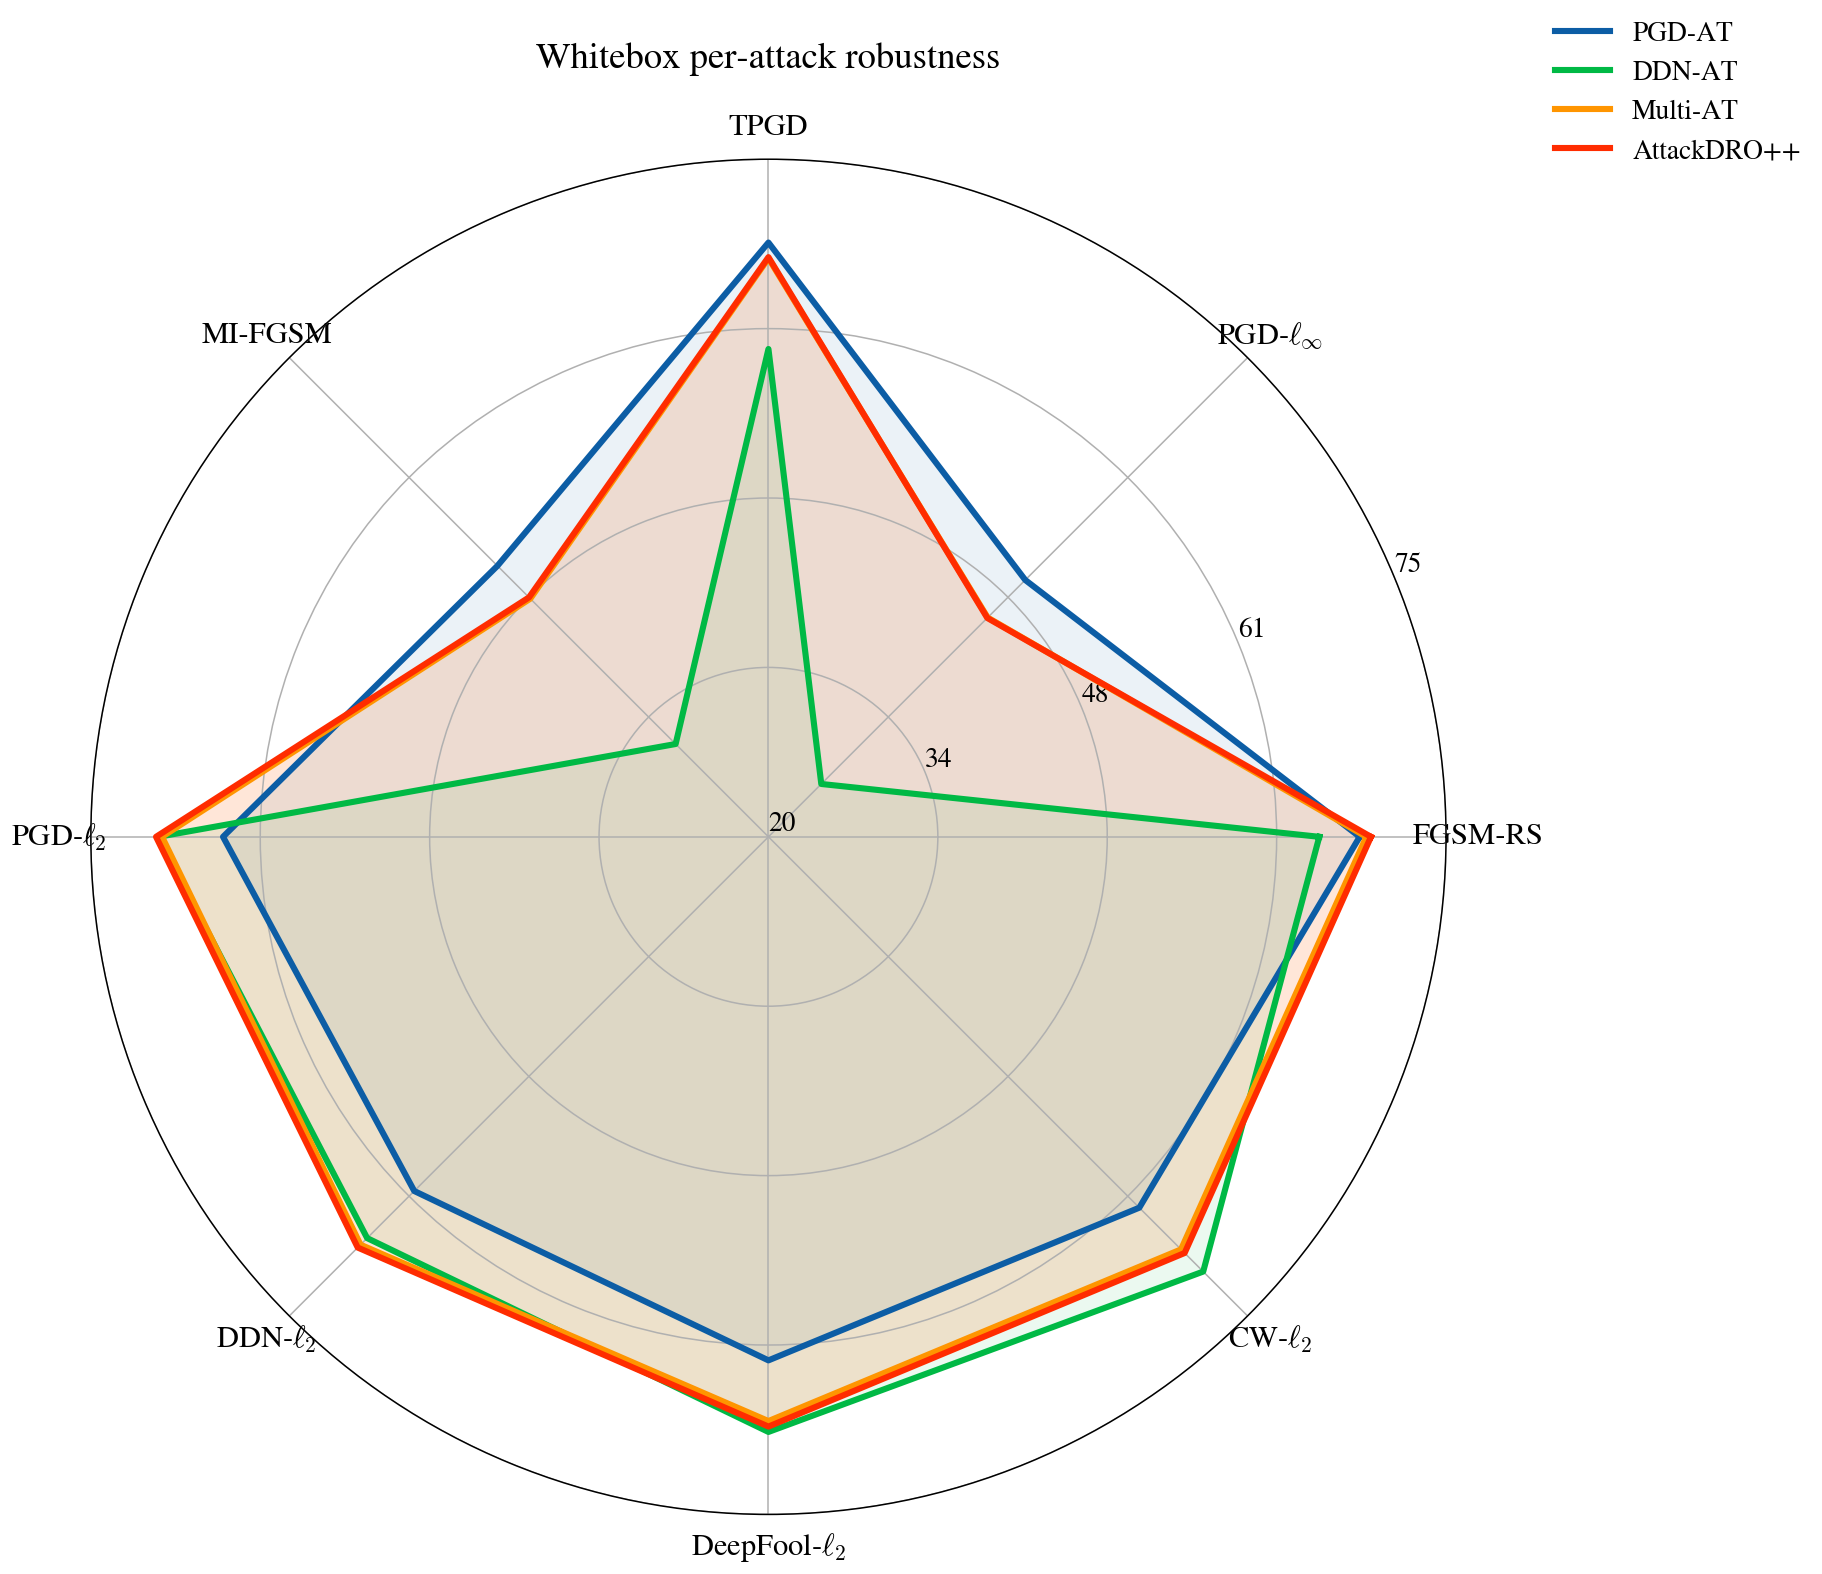
\includegraphics[width=0.78\linewidth]{figures/whitebox/whitebox_radar_per_attack_accuracy_n5.png}
\caption{Whitebox per-attack robustness profile averaged over five seeds. The radar plot compares PGD-AT, DDN-AT, Multi-AT, and AttackDRO++ (Ours) across the eight non-AutoAttack evaluation attacks. The shape of each curve highlights the specialization of the single-attack baselines and the more balanced profile of the multi-attack methods.}
\label{fig:ch6_whitebox_radar_per_attack_accuracy}
\end{figure}

\paragraph{Absolute per-class heatmaps with a shared scale.}
Before analyzing deltas, we first report the raw per-(class $\times$ attack) robust accuracy of each method. All four heatmaps use the same global color scale from 0\% to 100\%. This shared scale is important because it makes the maps visually comparable across methods: a darker cell always represents the same absolute robust accuracy, regardless of which method is being shown. 

\begin{figure}[H]
\centering
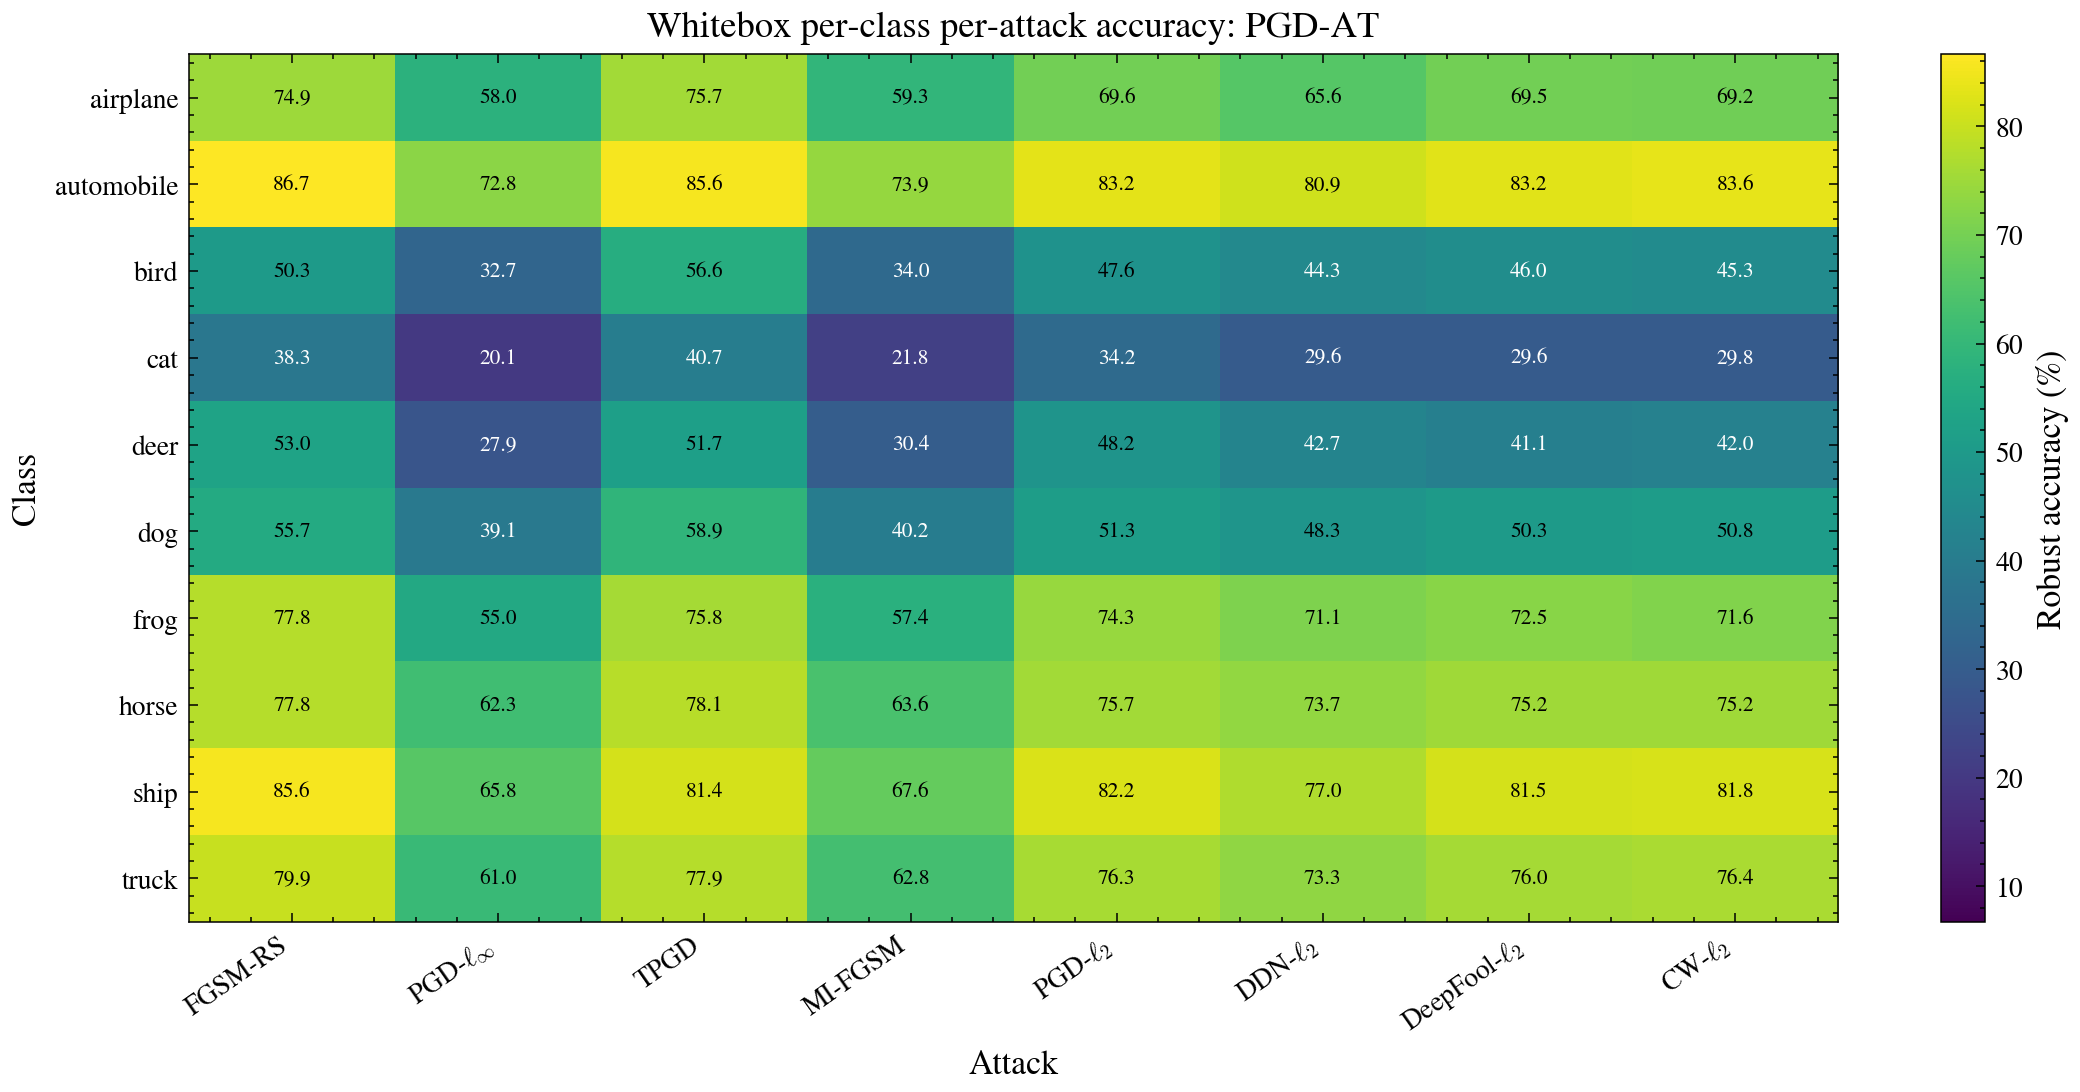
\includegraphics[width=\linewidth]{figures/whitebox/whitebox_per_class_attack_PGDAT_n5.png}
\caption{Absolute whitebox per-(class \(\times\) attack) robust accuracy
for PGD-AT. Cells report robust accuracy (\%).}
\label{fig:ch6_whitebox_abs_pgdat}
\end{figure}

\begin{figure}[H]
\centering
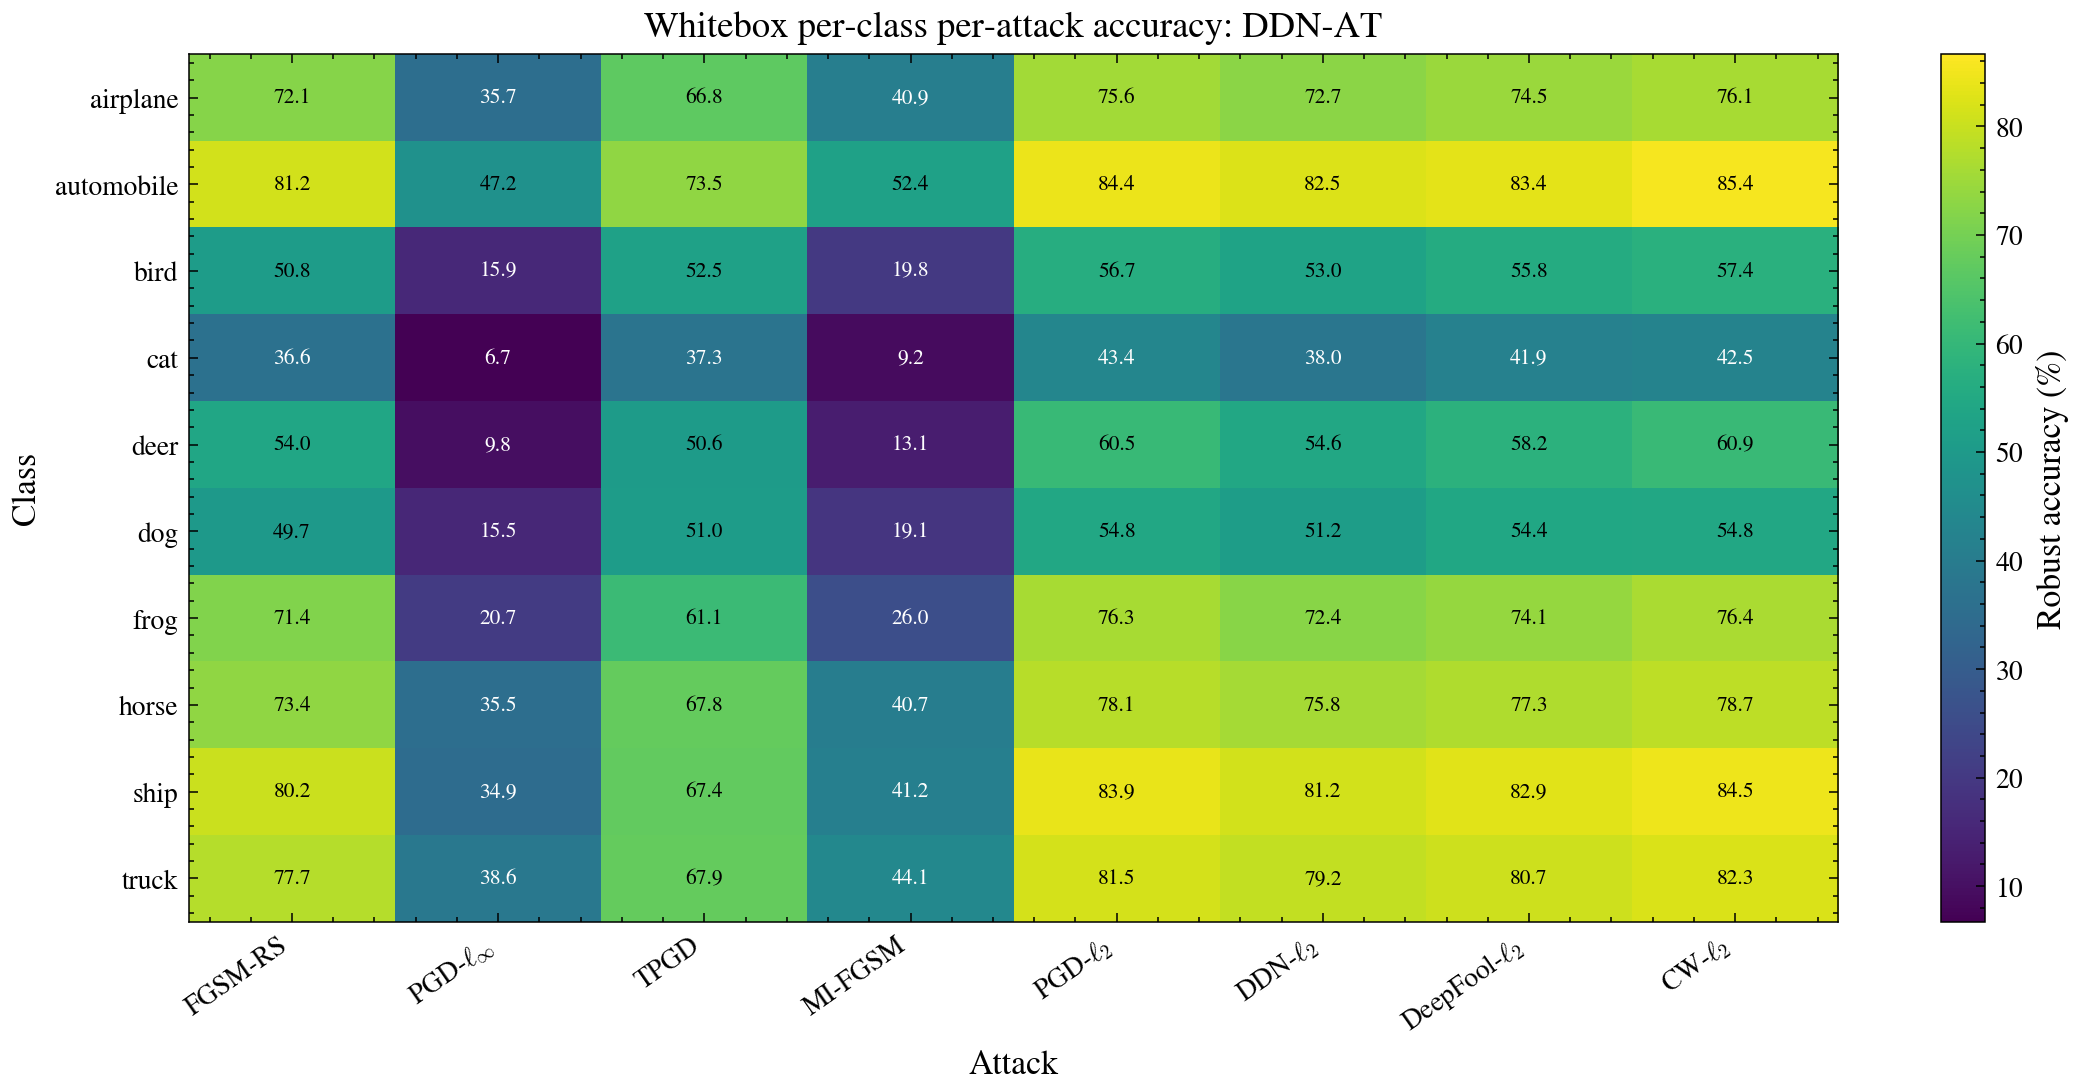
\includegraphics[width=\linewidth]{figures/whitebox/whitebox_per_class_attack_DDNAT_n5.png}
\caption{Absolute whitebox per-(class \(\times\) attack) robust accuracy
for DDN-AT. Cells report robust accuracy (\%).}
\label{fig:ch6_whitebox_abs_ddnat}
\end{figure}

\begin{figure}[H]
\centering
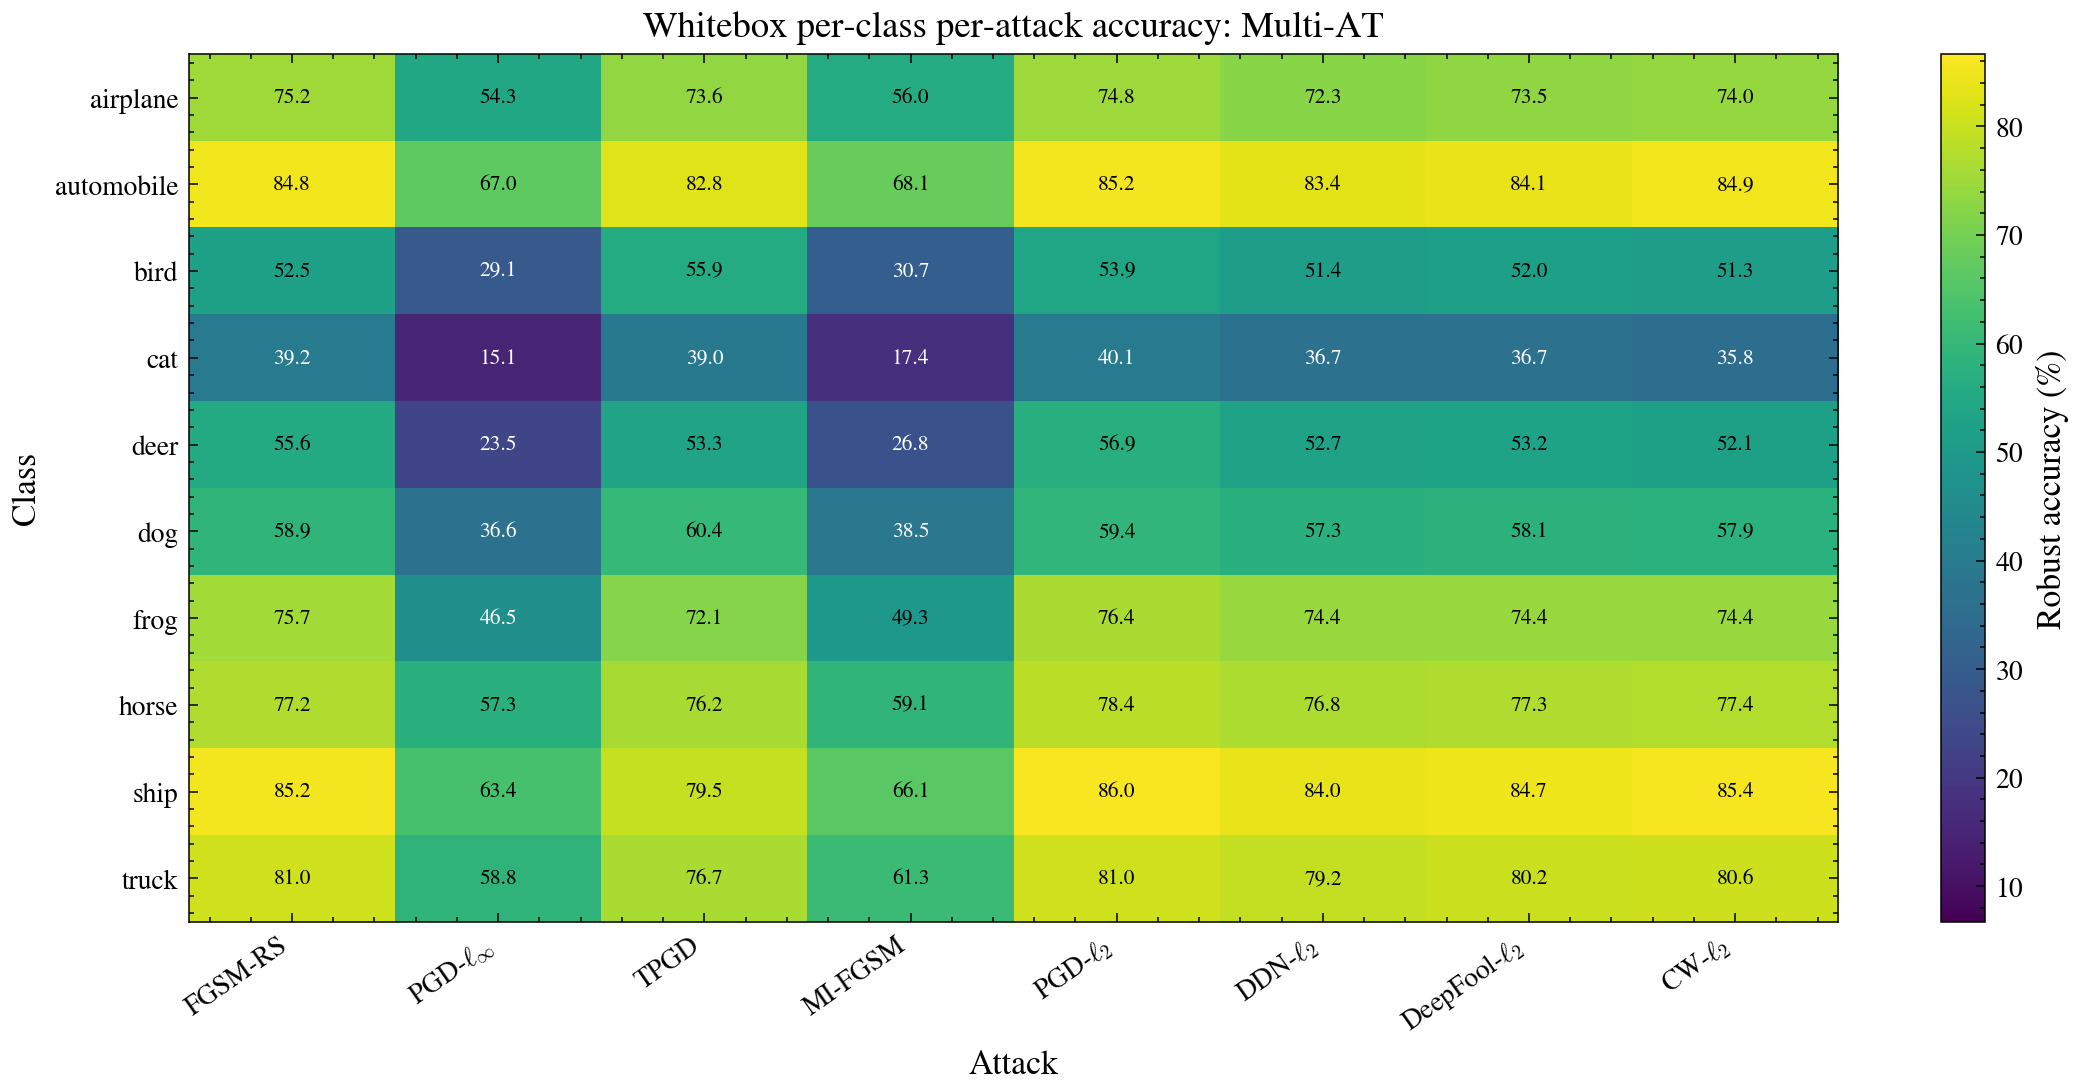
\includegraphics[width=\linewidth]{figures/whitebox/whitebox_per_class_attack_MultiAT_n5.png}
\caption{Absolute whitebox per-(class \(\times\) attack) robust accuracy
for Multi-AT. Cells report robust accuracy (\%).}
\label{fig:ch6_whitebox_abs_multiat}
\end{figure}

\begin{figure}[H]
\centering
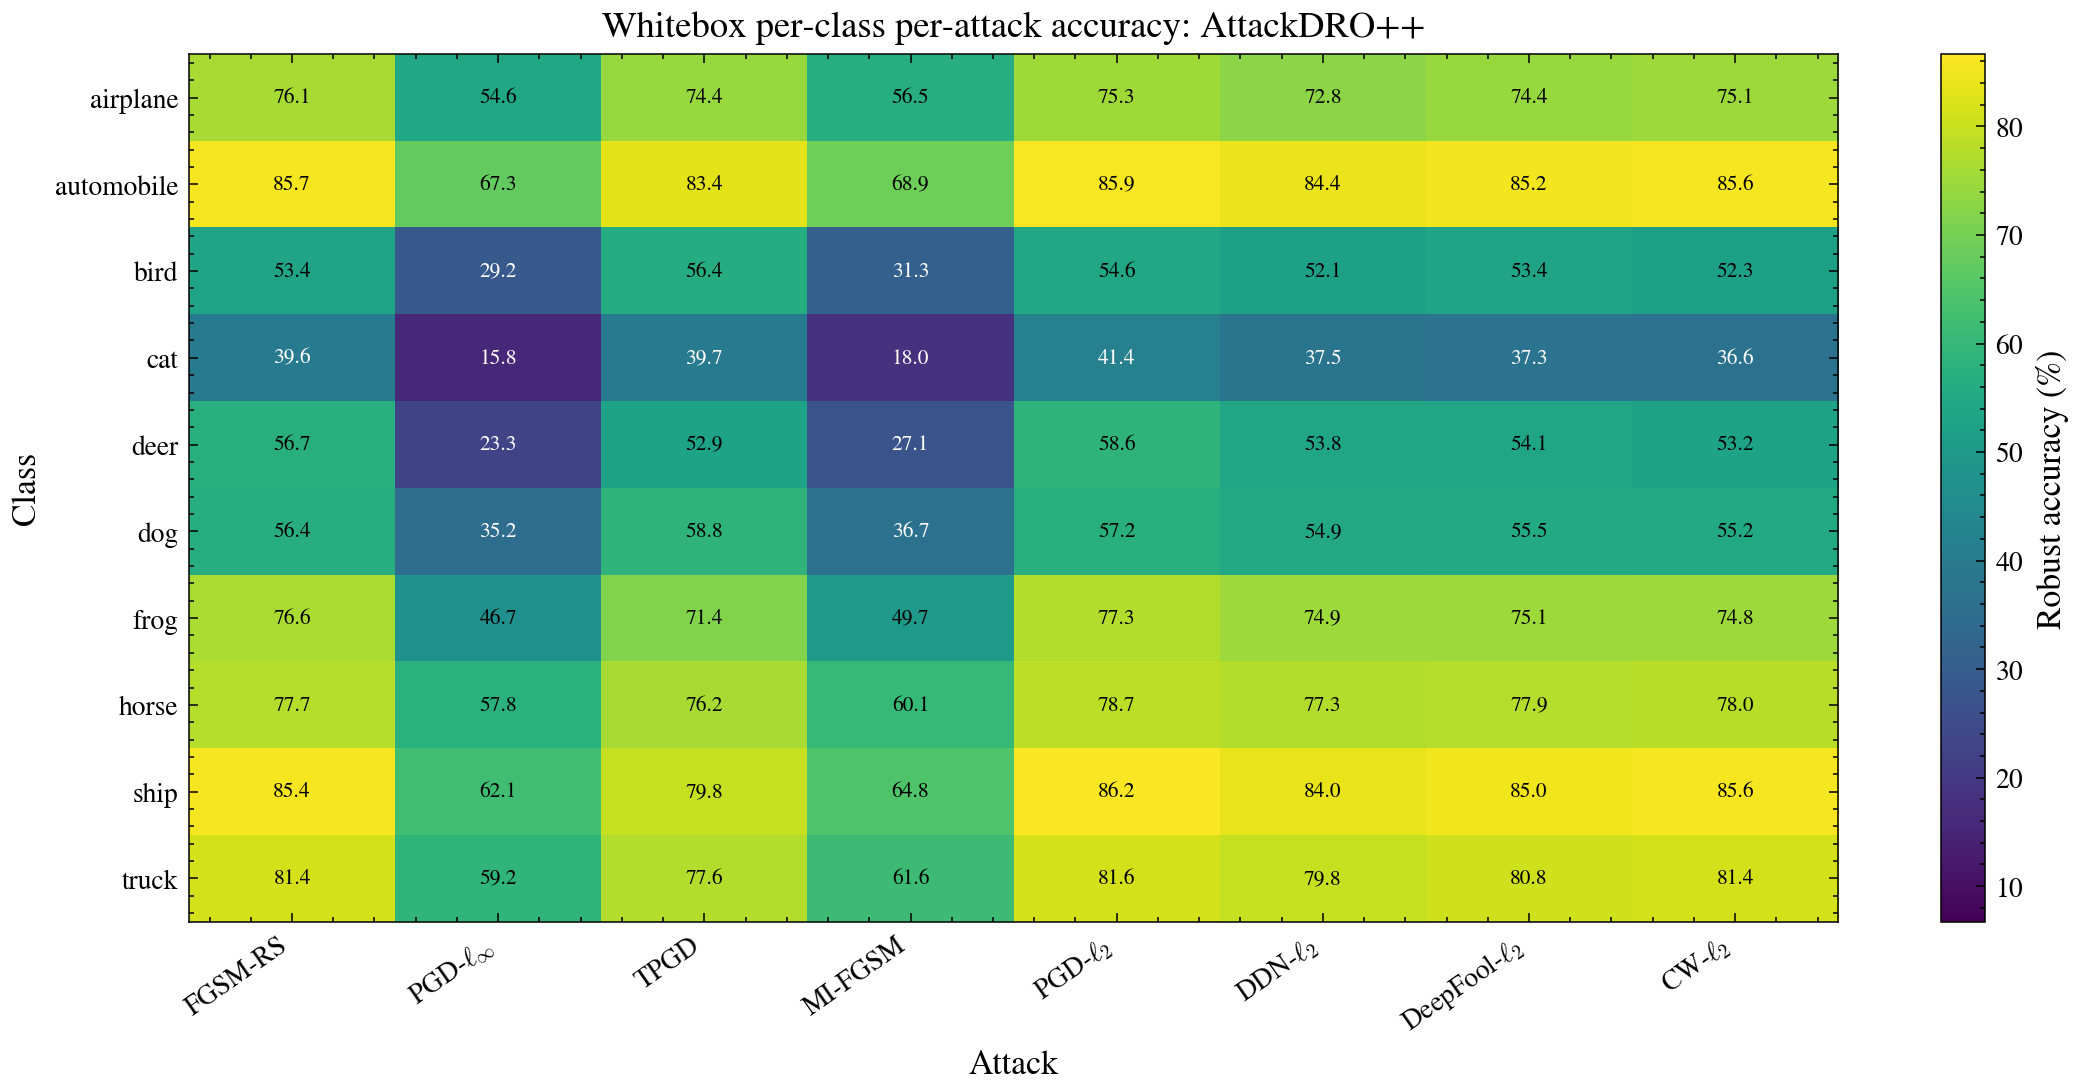
\includegraphics[width=\linewidth]{figures/whitebox/whitebox_per_class_attack_AttackDROpp_n5.png}
\caption{Absolute whitebox per-(class \(\times\) attack) robust accuracy
for AttackDRO++ (Ours). Cells report robust accuracy (\%).}
\label{fig:ch6_whitebox_abs_attackdropp}
\end{figure}
PGD-AT is stronger on several $\ell_\infty$ cells, while DDN-AT is more biased toward bounded $\ell_2$ attacks and visibly weaker on PGD-$\ell_\infty$ and MI-FGSM. Compared with the specialists, Multi-AT and AttackDRO++ show a more balanced cross-attack profile. AttackDRO++ largely preserves the Multi-AT structure while slightly lifting many cells, especially outside the hardest $\ell_\infty$ animal-class tail.

\subsection{Class-Level Gains and Persistent Difficulties}
\label{subsec:ch6_class_level_gains}

% TODO[Kiệt]:
% Goal:
% - Explain the main class-wise patterns without enumerating every class.
% Flow:
% - Identify broad high/low cells, then compare AttackDRO++ against Multi-AT and single-attack specialists.
% Include:
% - Reference `tab:ch6_whitebox_per_cell_summary` and the delta heatmaps.
% Avoid:
% - Unsupported causal claims about why individual CIFAR-10 classes are hard.
% Target length: 3-5 paragraphs.

Across all methods, the per-class robustness pattern is highly non-uniform. Classes such as \textit{automobile}, \textit{ship}, and \textit{truck} tend to remain easier under most attacks, while \textit{cat}, \textit{deer}, \textit{bird}, and \textit{dog} form the recurring hard tail. This pattern is consistent with the visual similarity and intra-class variation of CIFAR-10: animal classes often share local textures and backgrounds, so small adversarial perturbations can more easily move samples across nearby decision regions.

The hardest whitebox cells are concentrated in the $\ell_\infty$ iterative attacks. For AttackDRO++, the lowest cells are PGD-$\ell_\infty$ on \textit{cat} and \textit{deer}, followed by MI-FGSM on the same classes. This indicates that, even though AttackDRO++ improves the average multi-attack profile, the most difficult failure modes are still driven by strong $\ell_\infty$ optimization on semantically similar animal classes. In contrast, bounded $\ell_2$ attacks such as PGD-$\ell_2$, DDN-$\ell_2$, DeepFool-$\ell_2$, and CW-$\ell_2$ are generally less damaging for the proposed model than the strongest $\ell_\infty$ cells.

\paragraph{Attack-Class Delta Against Multi-AT Baseline}
Compared with Multi-AT, AttackDRO++ produces a broad but modest shift rather than a large change concentrated in a few cells. The mean per-cell gain is only $+0.281$ percentage points, but 67 out of 80 attack--class cells are positive.


\begin{figure}[H]
\centering
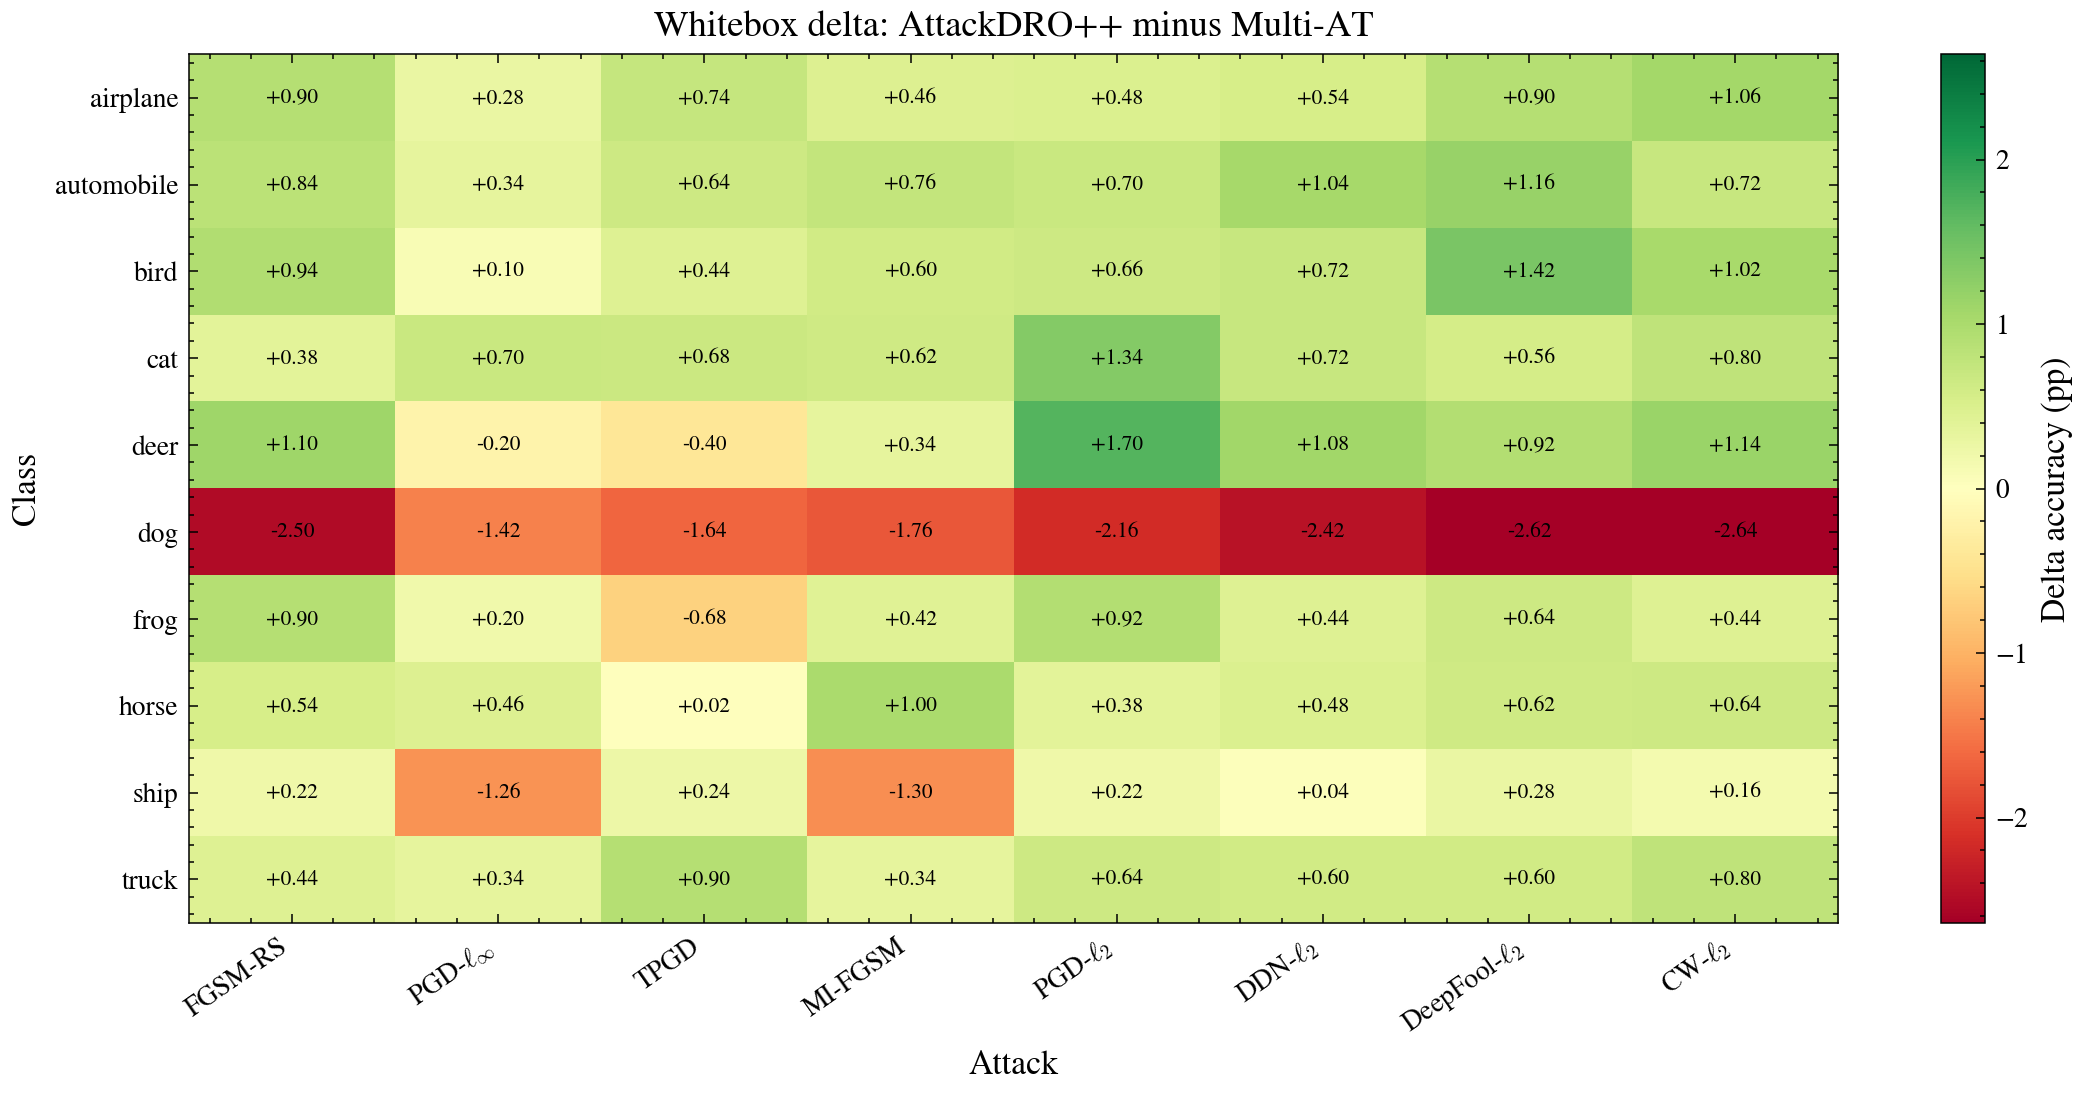
\includegraphics[width=\linewidth]{figures/whitebox/whitebox_delta_per_class_attack_AttackDROpp_vs_MultiAT_n5.png}
\caption{Whitebox per-(class $\times$ attack) delta of AttackDRO++ relative to Multi-AT. Each cell reports AttackDRO++ minus Multi-AT in percentage points, averaged over five seeds.}
\label{fig:ch6_whitebox_delta_vs_multiat}
\end{figure}

\paragraph{Attack-Class Delta Against Single-AT Baselines}

Table~\ref{tab:ch6_whitebox_per_cell_summary} summarizes the per-cell delta between AttackDRO++ and each baseline. The comparison against Multi-AT is the most important one because both methods train on the same source attacks and differ mainly in the group structure used for optimization. AttackDRO++ improves 67/80 cells over Multi-AT, with a mean gain of $+0.281$ percentage points and a bottom-10 lift of $+0.282$ percentage points. The gains are small, but they are widespread, which supports the interpretation that cluster-based DRO acts as a stabilizing refinement over uniform multi-attack training.

\begin{table}[H]
\centering
\caption{Per-(class $\times$ attack) whitebox comparison of AttackDRO++ against each baseline. $\Delta$ is computed as AttackDRO++ minus the baseline. Positive cells count the number of attack--class cells where $\Delta>0$ out of 80 total cells.}
\label{tab:ch6_whitebox_per_cell_summary}
\footnotesize
\setlength{\tabcolsep}{4.5pt}
\renewcommand{\arraystretch}{1.18}
\begin{tabular}{lccccc}
\toprule
Baseline
& Positive cells
& Mean
& Significant cells
& Bottom-10
& Main pattern \\
& $(\Delta>0)$
& $\Delta$ (pp)
& AttackDRO++ / Baseline
& lift (pp)
& \\
\midrule
Multi-AT
& 67/80
& $+0.281$
& 0 / 2
& $+0.282$
& Balanced refinement \\
PGD-AT
& 47/80
& $+1.782$
& 40 / 19
& $+0.726$
& Gains mainly on $\ell_2$ cells \\
DDN-AT
& 62/80
& $+5.781$
& 44 / 5
& $+15.710$
& Gains mainly on $\ell_\infty$ cells \\
\bottomrule
\end{tabular}

\end{table}

\begin{figure}[H]
\centering
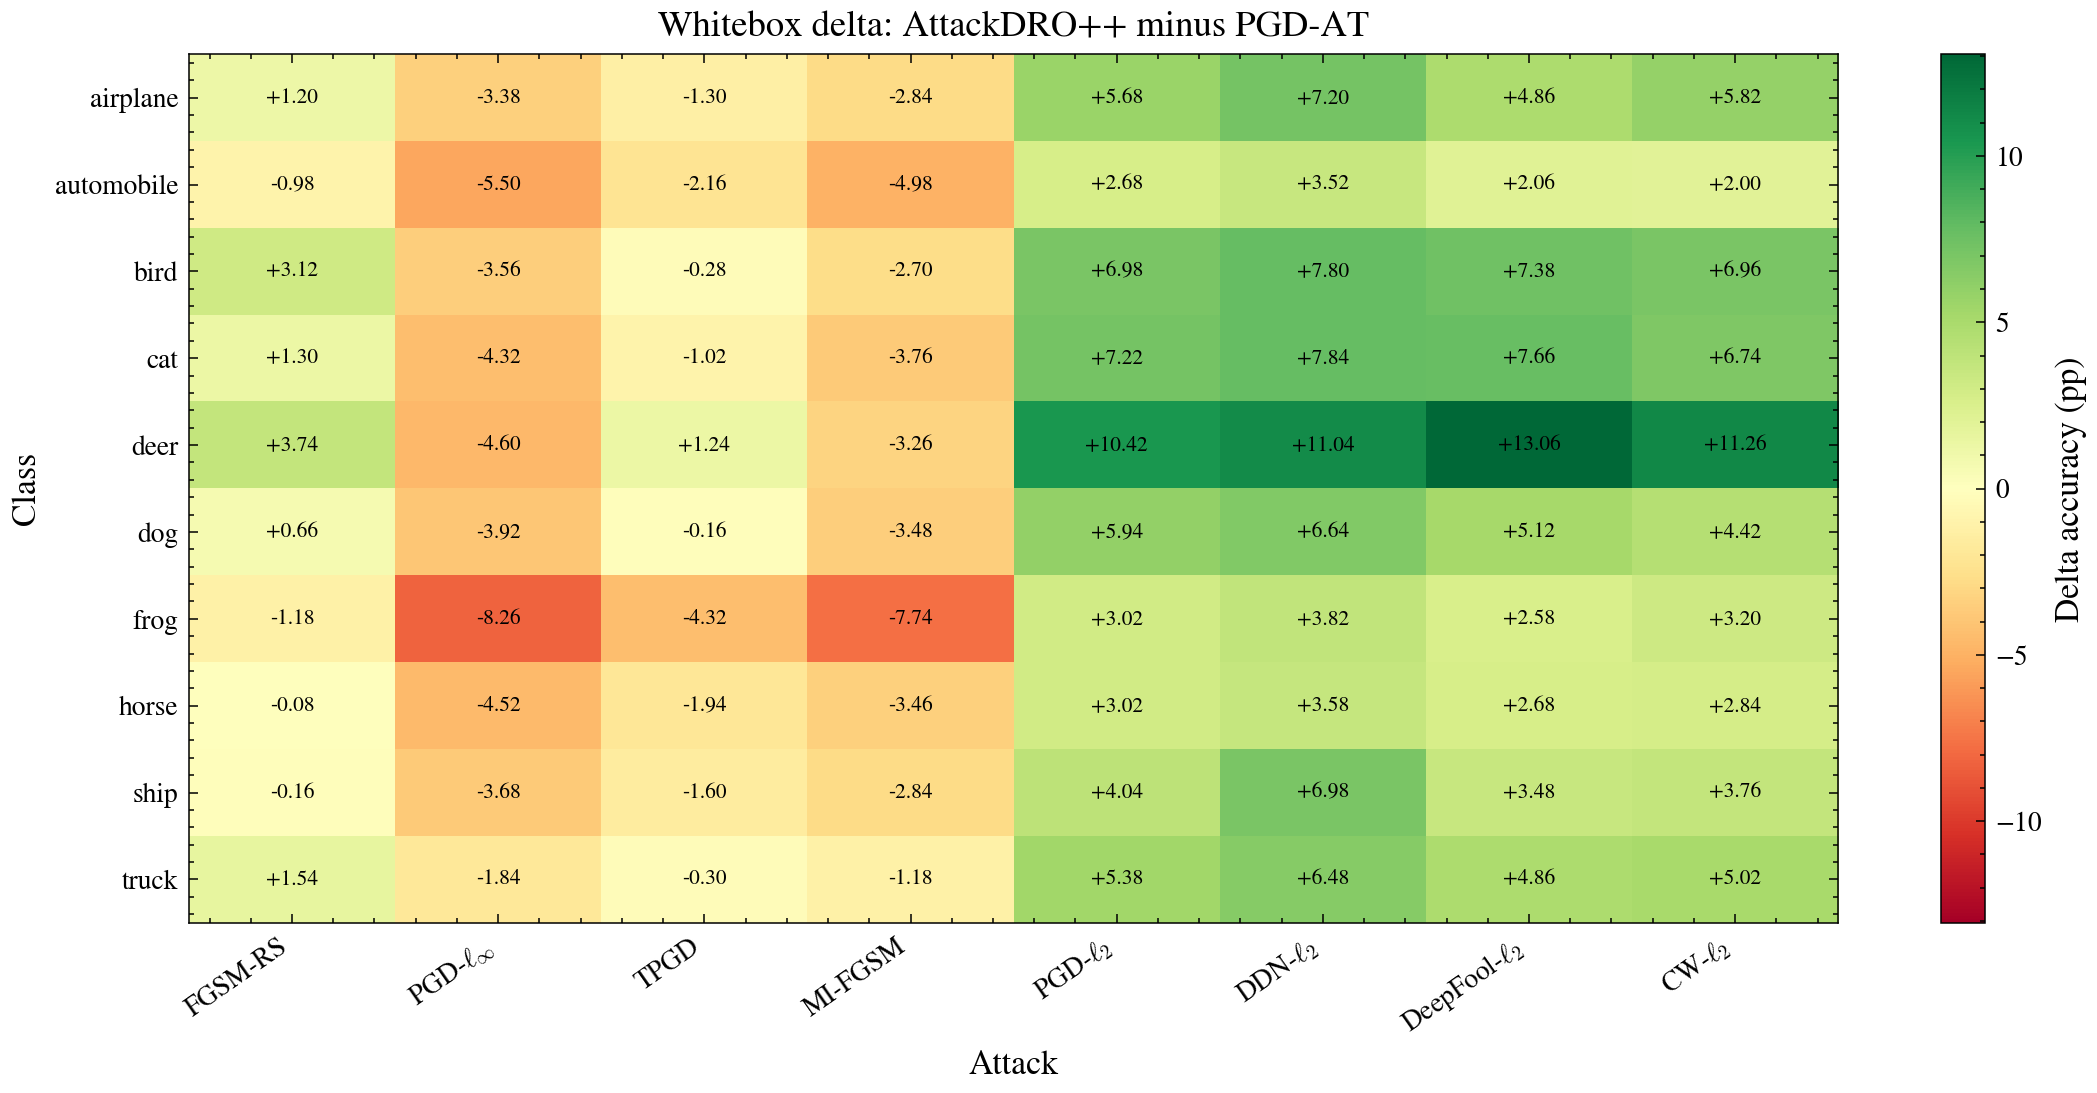
\includegraphics[width=\linewidth]{figures/whitebox/whitebox_delta_per_class_attack_AttackDROpp_vs_PGDAT_n5.png}
\caption{Whitebox per-(class $\times$ attack) delta of AttackDRO++ (Ours) relative to PGD-AT. Positive cells indicate where AttackDRO++ (Ours) improves over the PGD-$\ell_\infty$ specialist. Gains are concentrated mainly on bounded $\ell_2$ attacks, while PGD-AT remains stronger on several $\ell_\infty$ iterative cells.}
\label{fig:ch6_whitebox_delta_vs_pgdat}
\end{figure}

\begin{figure}[H]
\centering
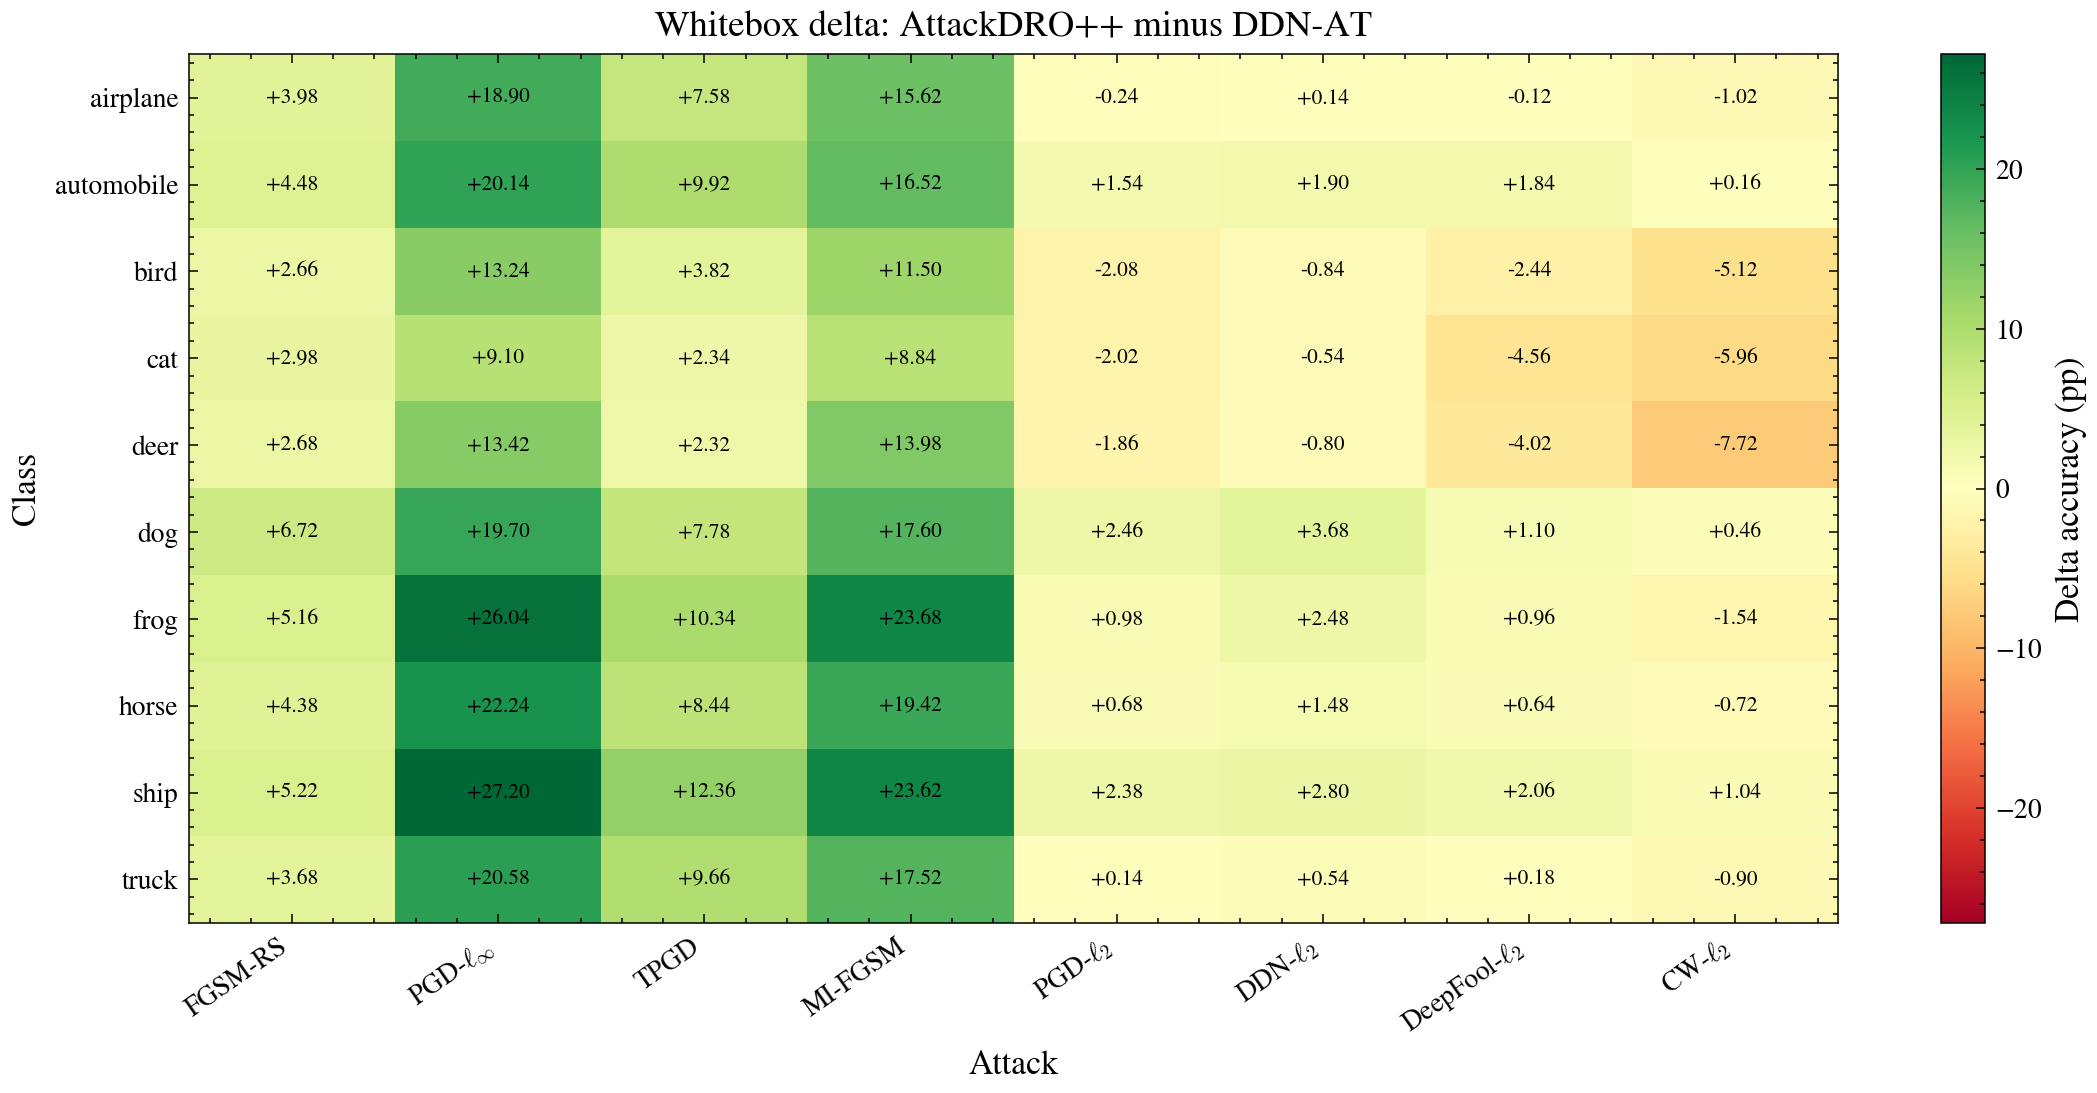
\includegraphics[width=\linewidth]{figures/whitebox/whitebox_delta_per_class_attack_AttackDROpp_vs_DDNAT_n5.png}
\caption{Whitebox per-(class $\times$ attack) delta of AttackDRO++ (Ours) relative to DDN-AT. The large positive cells under PGD-$\ell_\infty$ and MI-FGSM show that AttackDRO++ (Ours) substantially corrects the $\ell_\infty$ weakness of the DDN-$\ell_2$ specialist, while several negative cells remain on DDN-AT's preferred $\ell_2$ family.}
\label{fig:ch6_whitebox_delta_vs_ddnat}
\end{figure}

The comparison against PGD-AT shows the expected specialist trade-off. AttackDRO++ is positive in 47/80 cells and has a mean gain of $+1.782$ percentage points, but the gains and losses are not uniformly distributed. The largest improvements occur on bounded $\ell_2$ attacks, especially DeepFool-$\ell_2$, CW-$\ell_2$, DDN-$\ell_2$, and PGD-$\ell_2$ on hard animal classes such as \textit{deer}, \textit{cat}, and \textit{bird}. For example, the largest gains over PGD-AT appear on DeepFool-$\ell_2$ for \textit{deer} ($+13.06$ pp), CW-$\ell_2$ for \textit{deer} ($+11.26$ pp), and DDN-$\ell_2$ for \textit{deer} ($+11.04$ pp). Conversely, PGD-AT remains stronger on several $\ell_\infty$ cells, particularly PGD-$\ell_\infty$ and MI-FGSM for \textit{frog}, \textit{automobile}, \textit{horse}, and \textit{cat}. This confirms that PGD-AT is not weak in absolute terms; rather, it is specialized toward the $\ell_\infty$ geometry used during training.

The comparison against DDN-AT is even more asymmetric. AttackDRO++ improves 62/80 cells and gains $+5.781$ percentage points on average, with a large $+15.710$ percentage-point improvement on the bottom-10 cells. The largest improvements occur under $\ell_\infty$ attacks: PGD-$\ell_\infty$ on \textit{ship} ($+27.20$ pp), PGD-$\ell_\infty$ on \textit{frog} ($+26.04$ pp), MI-FGSM on \textit{frog} ($+23.68$ pp), and MI-FGSM on \textit{ship} ($+23.62$ pp). These large deltas show that DDN-AT develops a strong $\ell_2$ bias and leaves many $\ell_\infty$ attack--class cells under-protected. At the same time, DDN-AT remains stronger on some $\ell_2$ boundary/optimization cells, especially CW-$\ell_2$ and DeepFool-$\ell_2$ for \textit{deer}, \textit{cat}, and \textit{bird}. Thus, AttackDRO++ improves cross-attack balance but does not completely dominate the strongest single-norm specialist on its preferred family.

\paragraph{Attack-family interpretation.}

% TODO[Kiệt]:
% Goal:
% - Explain whether gains are balanced across attack families.
% Flow:
% - Compare source attacks, held-out `\ell_\infty`, and held-out `\ell_2` patterns.
% Include:
% - Reference the radar delta figure if kept in the main flow.
% Avoid:
% - Using metric shorthand in headings or unexplained captions.
% Target length: 2-4 paragraphs.

The attack-wise deltas make the specialization effect clear. Relative to PGD-AT, AttackDRO++ loses on PGD-$\ell_\infty$ and MI-FGSM on average, but gains strongly on the bounded $\ell_2$ attacks. Relative to DDN-AT, the pattern reverses: AttackDRO++ gains substantially on PGD-$\ell_\infty$, MI-FGSM, TPGD, and FGSM-RS, while being slightly weaker on CW-$\ell_2$ and DeepFool-$\ell_2$. 
The Multi-AT comparison is more balanced: most attack averages are positive, but the magnitudes are below one percentage point.

\begin{figure}[H]
\centering
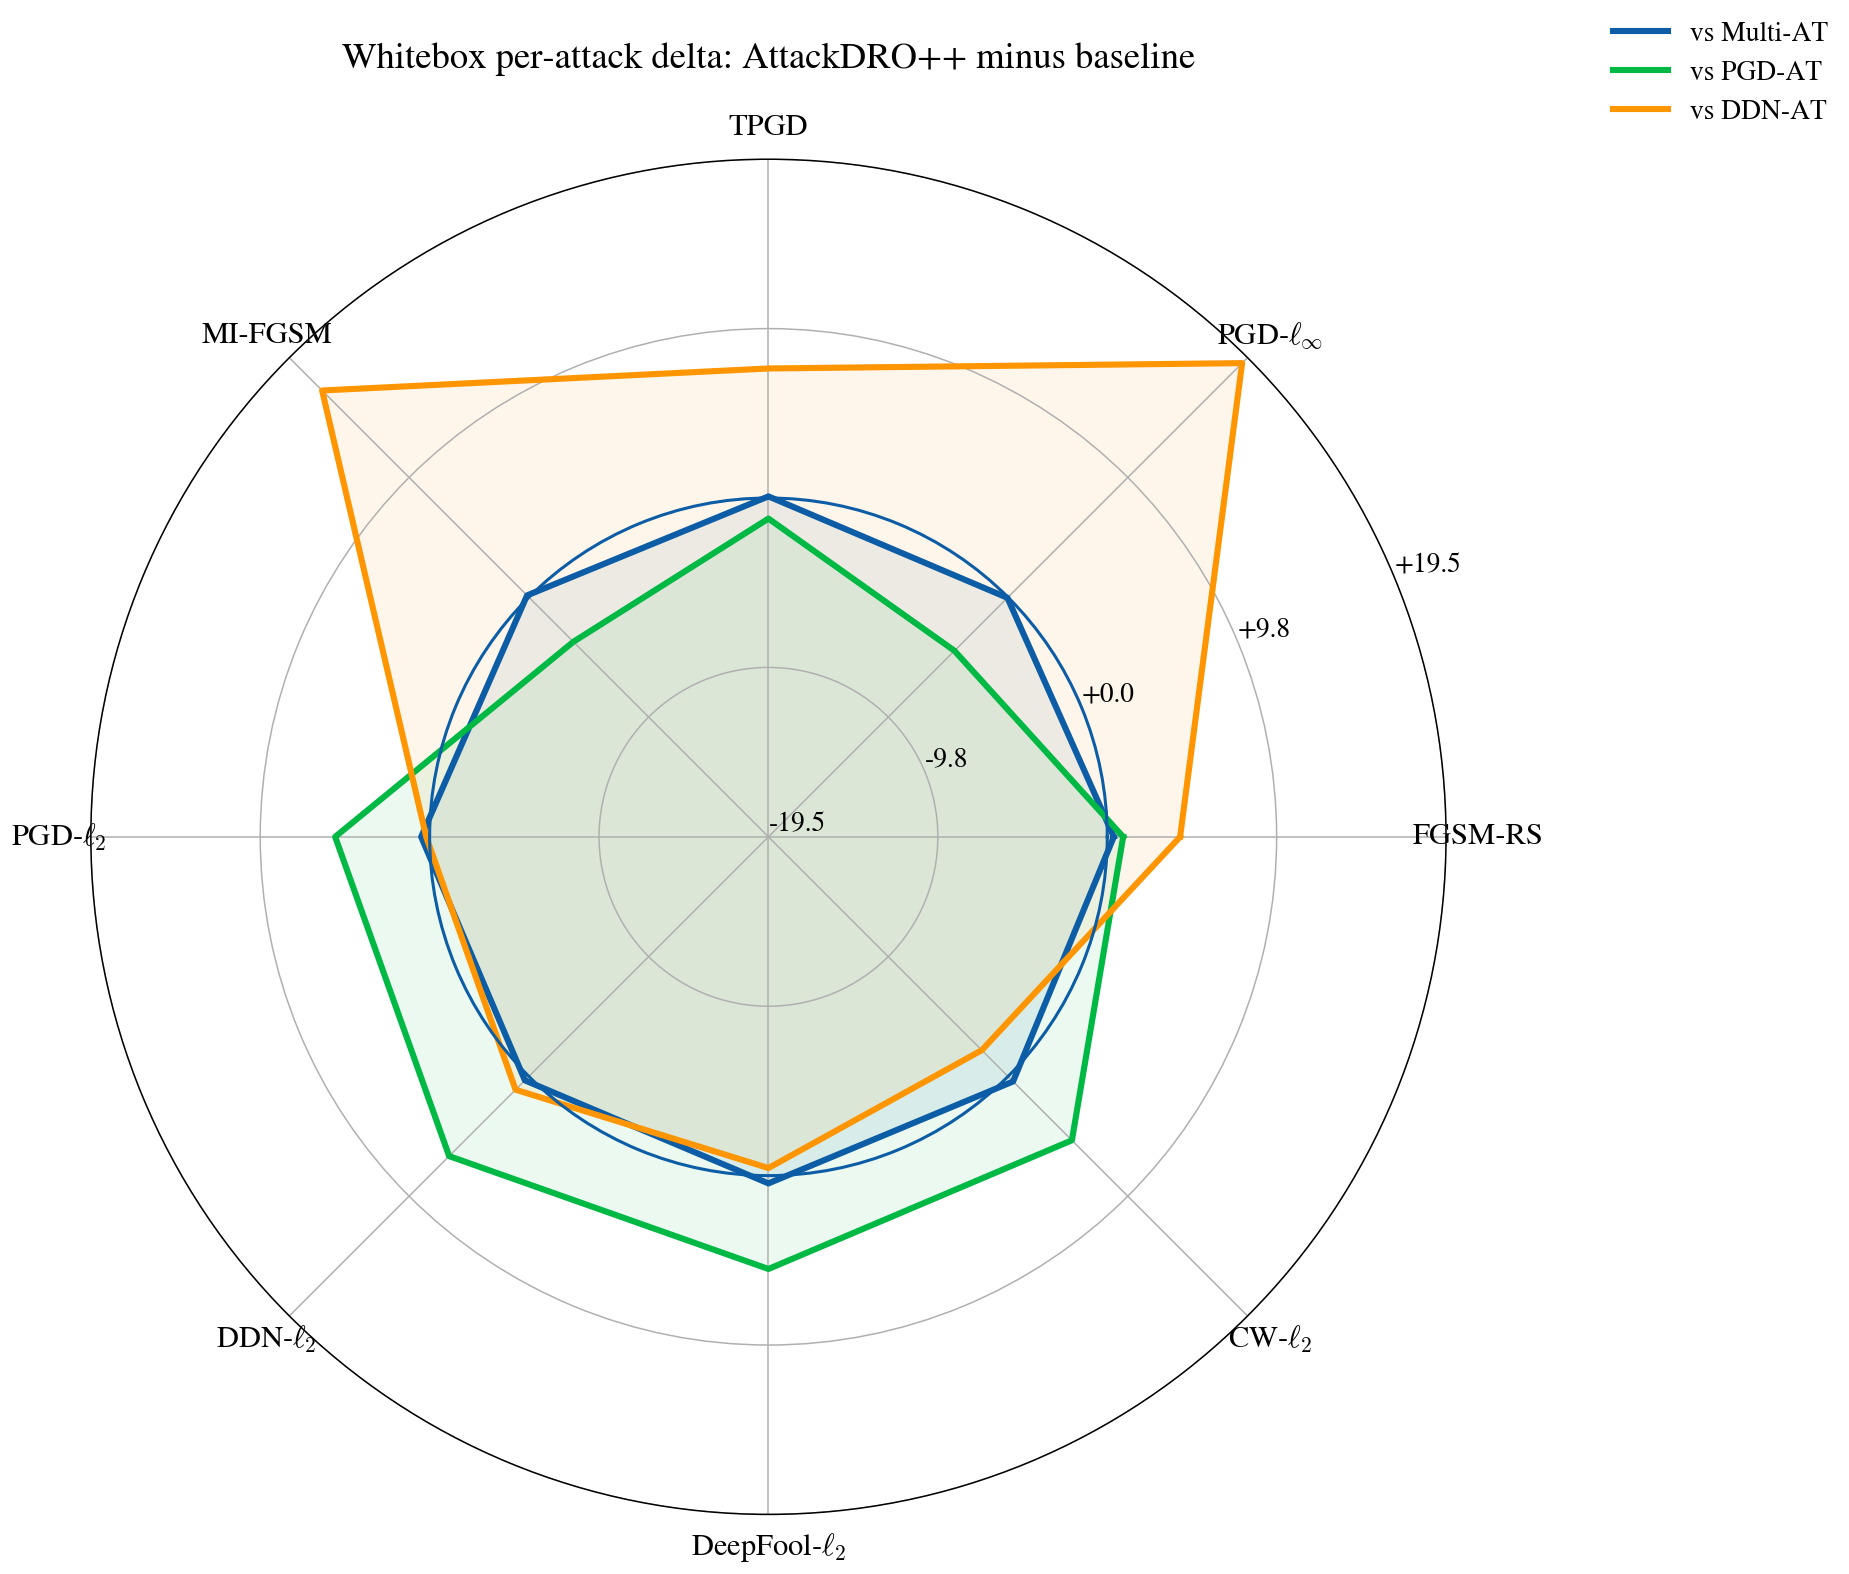
\includegraphics[width=\linewidth]{figures/whitebox/whitebox_radar_attackdropp_delta_vs_baselines_n5.png}
\caption{Attack-wise whitebox delta of AttackDRO++ relative to the three baselines.}
\label{fig:ch6_whitebox_radar_delta_vs_baselines}
\end{figure}
\vspace{-0.5cm}
This result supports the main claim of the chapter. AttackDRO++ should not be interpreted as a replacement for a single specialist when the deployment threat model is known exactly. Instead, it is a cross-attack robustness method: it sacrifices some of the peak strength of a specialist in exchange for a more even robustness profile across attacks and classes. 

\subsection{Tail-Class Robustness: Do the Weakest Cells Improve?}
\label{subsec:ch6_tail_class_robustness}

% TODO[Kiệt]:
% Goal:
% - Explain whether AttackDRO++ improves difficult tail cells, not only average cells.
% Flow:
% - Define Bottom-K locally or point to an earlier definition, then interpret the lift figure.
% Include:
% - Reference `fig:ch6_whitebox_bottomk_lift` if it remains in the main flow.
% Avoid:
% - Leaving `Bottom-K` as undefined shorthand.
% Target length: 2-3 paragraphs.

We next examine the weakest attack--class cells for each baseline, using
\(K \in \{5,10,20\}\). These cells capture localized failure modes that can be
hidden by mean accuracy. For Multi-AT, the weakest cells are mainly strong
\(\ell_\infty\) attacks, especially PGD-$\ell_\infty$ and MI-FGSM, on hard animal
classes such as \textit{cat}, \textit{deer}, and \textit{bird}. AttackDRO++
improves this tail only slightly: the bottom-10 lift is \(+0.282\) pp. Although
small, this shows that the average gain over Multi-AT is not obtained by
sacrificing its weakest cells.

\begin{figure}[H]
\centering
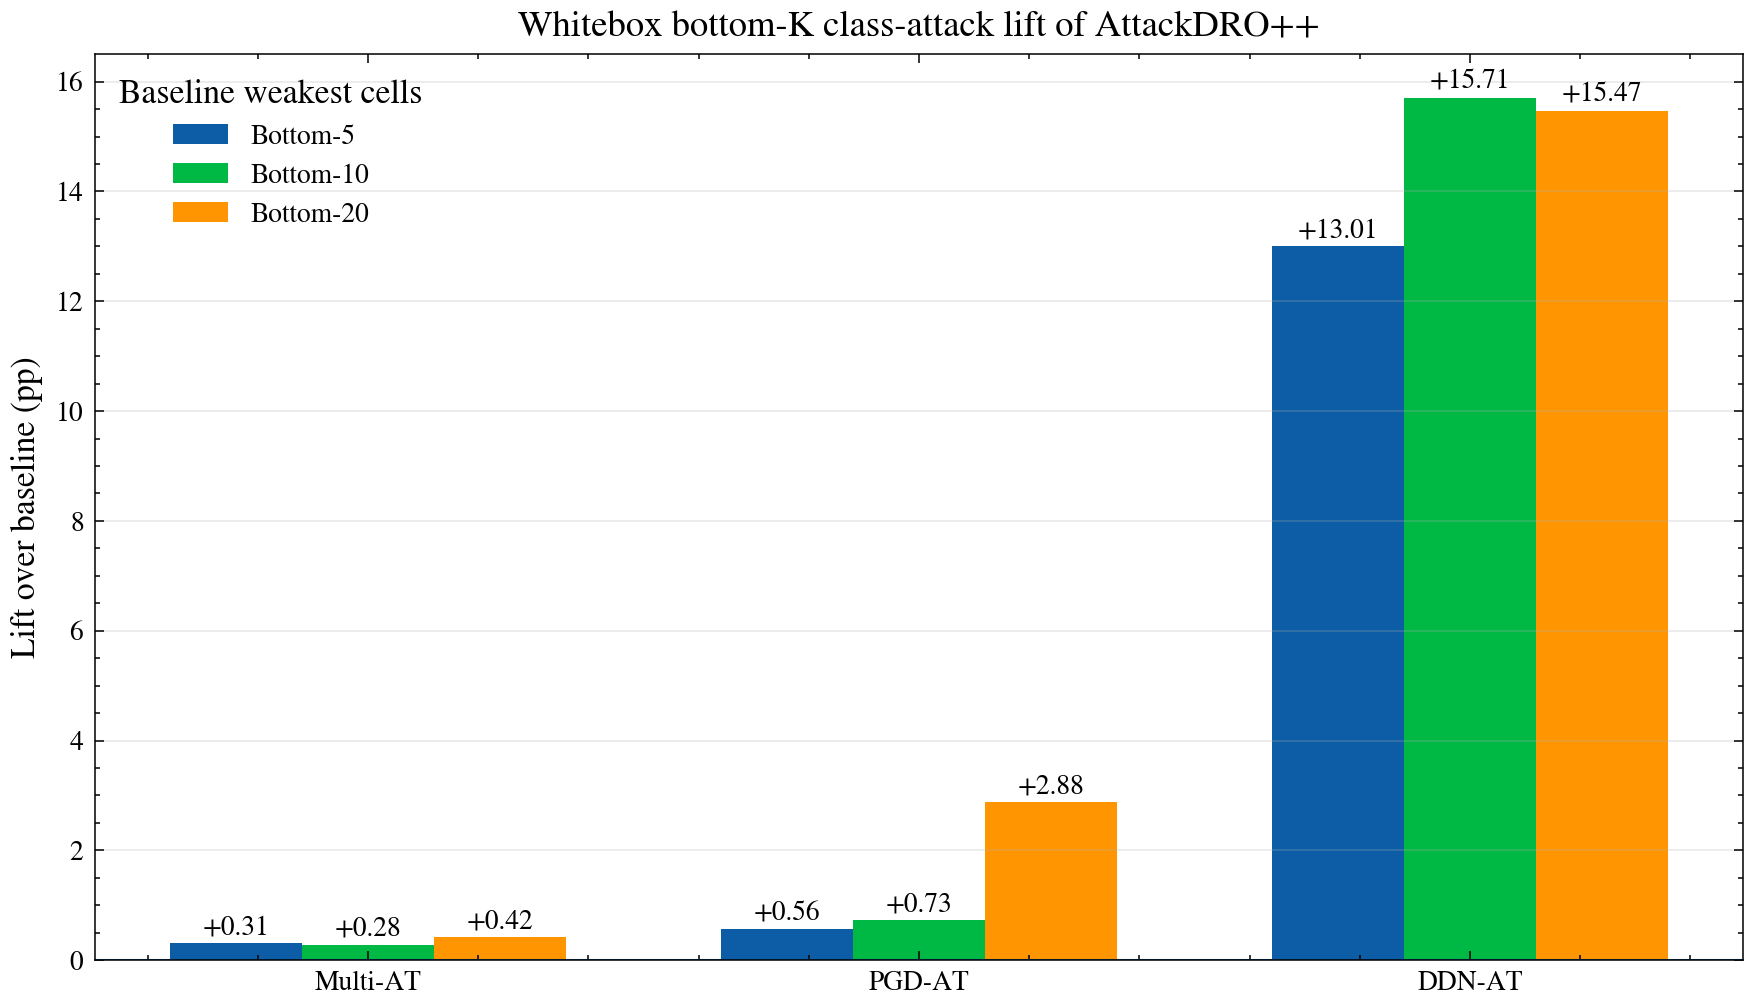
\includegraphics[width=0.64\linewidth]{figures/whitebox/whitebox_bottomk_lift_bar_n5.png}
\caption{Weakest-\(K\) whitebox class--attack lift of AttackDRO++ over each
baseline. For each baseline, the weakest-\(K\) cells are the lowest-accuracy
class--attack cells of that baseline; bars report AttackDRO++ minus the
baseline on those same cells.}
\label{fig:ch6_whitebox_bottomk_lift}
\end{figure}

The tail comparison is most pronounced against DDN-AT. Its weakest cells collapse
under \(\ell_\infty\)-oriented attacks, with the bottom-10 cells averaging only
\(15.602\%\). AttackDRO++ raises these same cells by \(+15.710\) pp, explaining
why it achieves a much more balanced whitebox profile than the \(\ell_2\)
specialist, even though DDN-AT remains competitive on several \(\ell_2\) cells.

Against PGD-AT, the lift is smaller but still positive: \(+0.726\) pp on the
bottom-10 cells. PGD-AT's weakest cells include several bounded \(\ell_2\)
attacks on difficult classes such as \textit{cat} and \textit{deer}; AttackDRO++
reduces many of these failures, indicating that multi-attack training and the
Cluster-DRO component help mitigate the cross-norm weakness of PGD-only training.

Overall, the weakest-cell analysis supports the aggregate conclusion from
Section~\ref{sec:ch6_whitebox}: AttackDRO++ gives a broad but modest refinement
over Multi-AT, substantially corrects the \(\ell_\infty\) tail weakness of
DDN-AT, and reduces the \(\ell_2\) tail weakness of PGD-AT.

The class-wise whitebox analysis shows where the aggregate gains appear and
which hard cells remain. It still evaluates attacks generated directly against
the target checkpoint, so it does not answer whether the same robustness pattern
holds when adversarial examples are crafted on a different model. The next
section therefore moves to the graybox transfer protocol from
Section~\ref{sec:ch5_graybox_protocol}.


% ─────────────────────────────────────────────────────────────────────────────
\newpage
\section{Graybox Robustness Across Surrogate Models}
\label{sec:ch6_graybox}

% TODO[Kiệt]:
% Goal:
% - Explain graybox robustness as transfer behavior, not just another accuracy table.
% Flow:
% - Start with protocol sanity, then transfer matrices, pairwise comparisons, gap analysis, per-cell analysis, and decomposition.
% Include:
% - Cite active figures/tables from docs/04_figure_table_registry.md, especially currently unreferenced graybox tables/figures if kept.
% Avoid:
% - Overclaiming deployment transfer beyond the surrogate/target protocol.
% Target length: 6-9 pages depending on consolidation.
% ─────────────────────────────────────────────────────────────────────────────

The whitebox results in Section~\ref{sec:ch6_whitebox} show that
AttackDRO++ improves average and held-out robustness over Multi-AT on
\(n=20\) paired seeds. We next test whether this gain also holds under
cross-model transfer, using the graybox protocol of
Section~\ref{sec:ch5_graybox_protocol}. In this setting, adversarial examples
are generated on one checkpoint and evaluated on an independently trained
target checkpoint.

\paragraph{Random-seed checkpoint panel and whitebox sanity check.}

% TODO[Kiệt]:
% Goal:
% - Justify the random-seed checkpoint panel and show it is consistent with the main whitebox trends.
% Flow:
% - Explain the fixed random-seed panel, then interpret `tab:ch6_graybox_whitebox_sanity`.
% Include:
% - State clearly that this is a sanity check, not the main 20-seed whitebox result.
% Avoid:
% - Repeating full Chapter 6.1 results.
% Target length: 2-3 paragraphs.

The graybox analysis uses 20 random-seed checkpoints to define the
surrogate--target evaluation panel. These checkpoints come from four method
families evaluated across five random seeds each and are fixed before graybox
transfer is analyzed. The diagonal sanity check below compares this
random-seed checkpoint panel against the full whitebox panel to verify that the
main method ordering is preserved.

The diagonal entries of the graybox table correspond to the case where
the surrogate and target are the same checkpoint. We use these entries as
a whitebox sanity check. They need not match the main whitebox evaluation
exactly, because the graybox cache uses a balanced
125-image-per-class-per-attack split instead of the full test set for
each attack. However, they should preserve the same method ordering and
remain close in absolute value.

\begin{table}[H]
\centering
\caption{Whitebox sanity check from the graybox pipeline. The \(n=5\)
columns use diagonal graybox entries, where surrogate and target are the
same checkpoint. The \(n=20\) columns report the main whitebox results
from Table~\ref{tab:ch6_aggregate_results}.}
\label{tab:ch6_graybox_whitebox_sanity}
\small
\setlength{\tabcolsep}{6pt}
\renewcommand{\arraystretch}{1.08}
\begin{tabular}{lrrrr}
\toprule
Target method
& Mean(8) \(n=5\)
& Worst(8) \(n=5\)
& Mean(8) \(n=20\)
& Worst(8) \(n=20\) \\
\midrule
PGD-AT
& $61.524$ & $\mathbf{50.384}$ & $60.499$ & $\mathbf{49.656}$ \\
DDN-AT
& $56.922$ & $25.568$ & $56.226$ & $25.957$ \\
Multi-AT
& $62.458$ & $45.584$ & $62.045$ & $45.082$ \\
AttackDRO++ (Ours)
& $\mathbf{62.642}$ & $45.088$ & $\mathbf{62.324}$ & $45.079$ \\
\bottomrule
\end{tabular}
\end{table}

The Mean(8) ordering is identical on both panels --- AttackDRO++ $>$
Multi-AT $>$ PGD-AT $>$ DDN-AT --- and absolute values agree to within
$1.0$~pp. More importantly, the paired Mean(8) delta of AttackDRO++ minus
Multi-AT is $+0.184$~pp on the $n=5$ graybox panel and
$+0.279$~pp on the full $n=20$ panel: both are positive and of the same
order of magnitude. The graybox cache is therefore consistent with the
main evaluation protocol and supports the cross-method analyses below.

\subsection{Cross-Method Transfer Structure}
\label{subsec:ch6_graybox_transfer_structure}

% TODO[Kiệt]:
% Goal:
% - Explain how to read the graybox transfer matrices and what off-diagonal transfer means.
% Flow:
% - Define row/column roles, then interpret aggregate and per-attack matrices.
% Include:
% - Reference `fig:ch6_graybox_transfer_matrix`, `fig:ch6_graybox_transfer_linf`, and `fig:ch6_graybox_transfer_l2`.
% Avoid:
% - Treating diagonal whitebox cells as graybox evidence.
% Target length: 3-5 paragraphs.

We aggregate the per-attack per-class transfer table into a method-level
$4 \times 4$ transfer matrix. Rows index the target method being evaluated, and columns index the
surrogate method that generates adversarial examples. Each cell reports
the target robust accuracy averaged over all matching target--surrogate
seed pairs and the eight evaluation attacks. Higher values indicate that
the row target is more robust to adversarial examples crafted on the
column surrogate.

\begin{figure}[H]
\centering
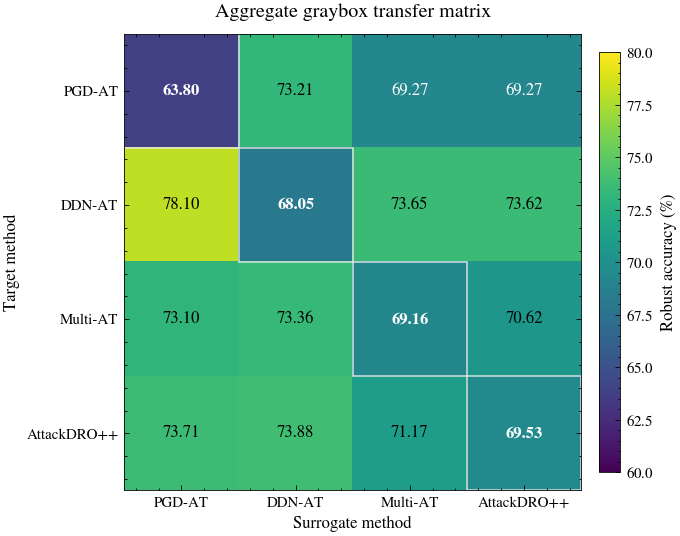
\includegraphics[width=0.78\linewidth]{figures/graybox/graybox_transfer_matrix_4method_aggregate_science_clean.png}
\caption{Method-level graybox transfer matrix on the \(n=5\) panel.
Rows are target methods and columns are surrogate methods. Cell values
are robust accuracy (\%) averaged over seeds and the eight evaluation
attacks.}
\label{fig:ch6_graybox_transfer_matrix}
\end{figure}

Two structural patterns are visible. First, rows ranked by mean
off-diagonal accuracy give DDN-AT ($75.12\%$) $>$ AttackDRO++ ($72.92\%$)
$>$ Uniform Multi-AT ($72.36\%$) $>$ PGD-AT ($70.59\%$). The DDN-AT
row is highest not because DDN-AT is the strongest defense --- its
whitebox Mean(8) is the lowest of the four --- but because $\ell_\infty$
adversarial examples generated by other surrogates transfer poorly to a
DDN-AT target whose decision boundary is shaped by $\ell_2$ training.
Section~\ref{subsec:ch6_paired_graybox_comparisons} quantifies this structural inflation
explicitly through the whitebox--graybox gap. Second, the AttackDRO++
row is consistently above the Uniform Multi-AT row for every surrogate,
with cross-method gaps ranging from $+0.17$~pp (DDN-AT surrogate) to
$+0.61$~pp (PGD-AT surrogate). The whitebox advantage of AttackDRO++
over Uniform Multi-AT therefore persists when adversarial examples are
crafted on independently trained surrogates.

The aggregate transfer matrix hides important attack-family structure.
Figures~\ref{fig:ch6_graybox_transfer_linf} and~\ref{fig:ch6_graybox_transfer_l2}
therefore disaggregate the transfer behavior into the four
\(\ell_\infty\)-oriented attacks and the four \(\ell_2\)-oriented attacks.
This grouping makes the specialist behavior more explicit. 

\begin{figure}[H]
\centering
\begin{minipage}{0.48\linewidth}
  \centering
  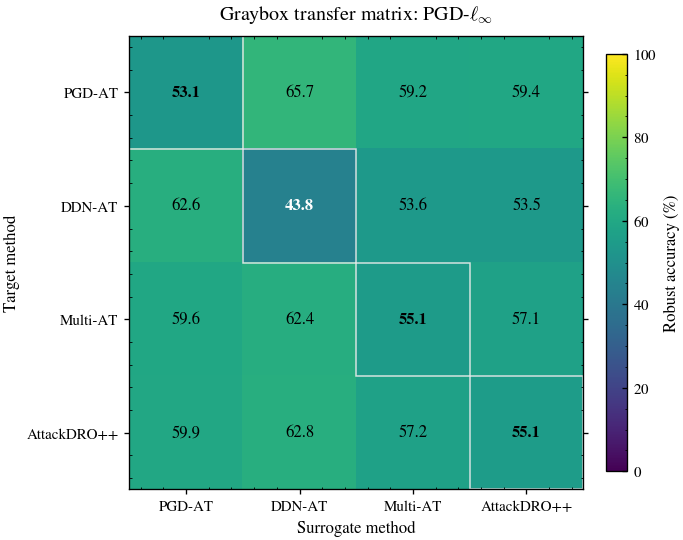
\includegraphics[width=\linewidth]{figures/graybox/transfer_matrix_4method_pgd20_ce_science_clean.png}
  \\ \footnotesize (a) PGD-\(\ell_\infty\)
\end{minipage}\hfill
\begin{minipage}{0.48\linewidth}
  \centering
  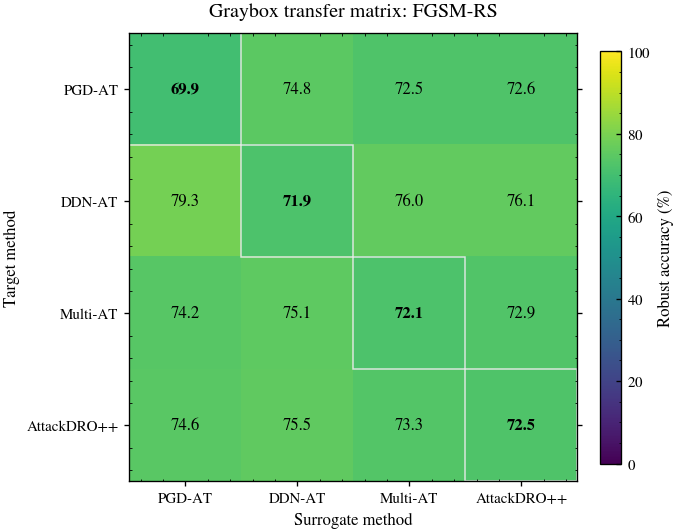
\includegraphics[width=\linewidth]{figures/graybox/transfer_matrix_4method_fgsm_rs_science_clean.png}
  \\ \footnotesize (b) FGSM-RS
\end{minipage}

\vspace{0.6em}

\begin{minipage}{0.48\linewidth}
  \centering
  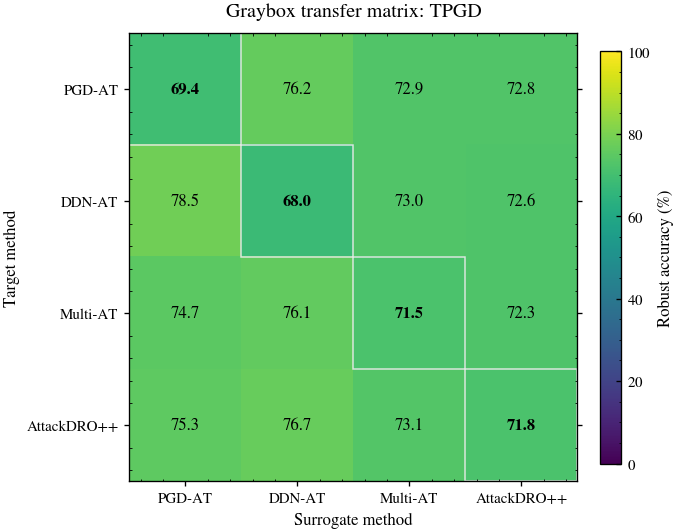
\includegraphics[width=\linewidth]{figures/graybox/transfer_matrix_4method_tpgd_science_clean.png}
  \\ \footnotesize (c) TPGD
\end{minipage}\hfill
\begin{minipage}{0.48\linewidth}
  \centering
  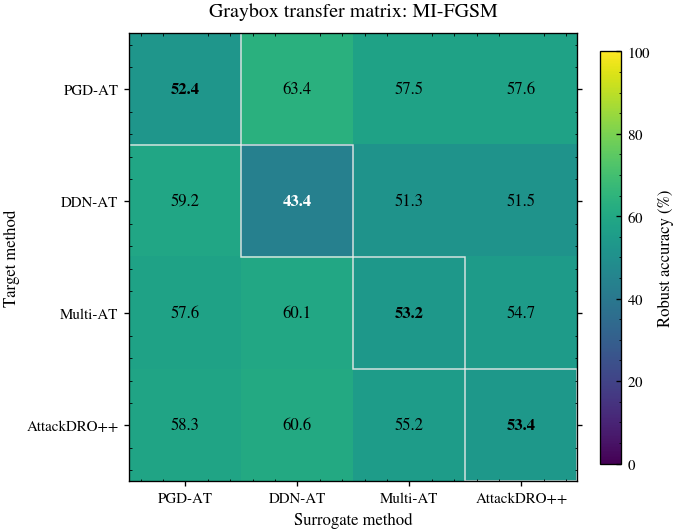
\includegraphics[width=\linewidth]{figures/graybox/transfer_matrix_4method_mifgsm_science_clean.png}
  \\ \footnotesize (d) MI-FGSM
\end{minipage}

\caption{Per-attack graybox transfer matrices for the
\(\ell_\infty\)-oriented attacks. Rows are target methods and columns
are surrogate methods; cells report robust accuracy (\%).}
\label{fig:ch6_graybox_transfer_linf}
\end{figure}

On the
\(\ell_\infty\) attacks, this advantage disappears: PGD-AT and
AttackDRO++ are more competitive, and AttackDRO++ remains closer to the
balanced Multi-AT profile. Thus, the per-attack matrices show that
DDN-AT's strong graybox row average should be interpreted as
family-specific transfer specialization rather than uniform robustness.

\begin{figure}[H]
\centering
\begin{minipage}{0.48\linewidth}
  \centering
  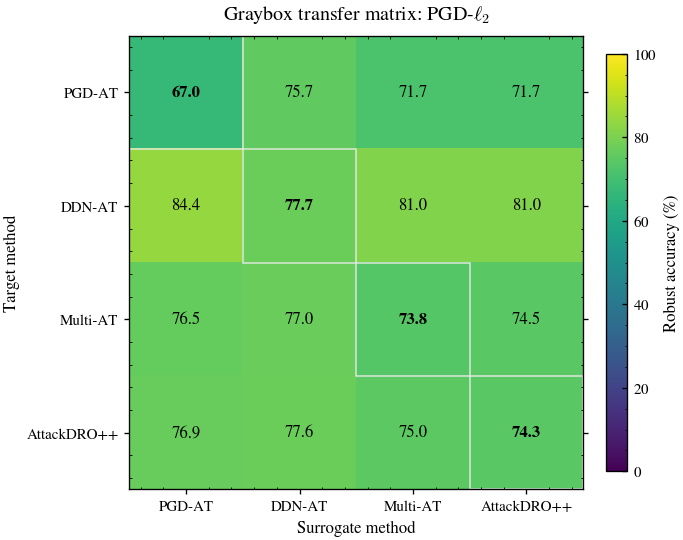
\includegraphics[width=\linewidth]{figures/graybox/transfer_matrix_4method_pgd_l2_science_clean.png}
  \\ \footnotesize (a) PGD-\(\ell_2\)
\end{minipage}\hfill
\begin{minipage}{0.48\linewidth}
  \centering
  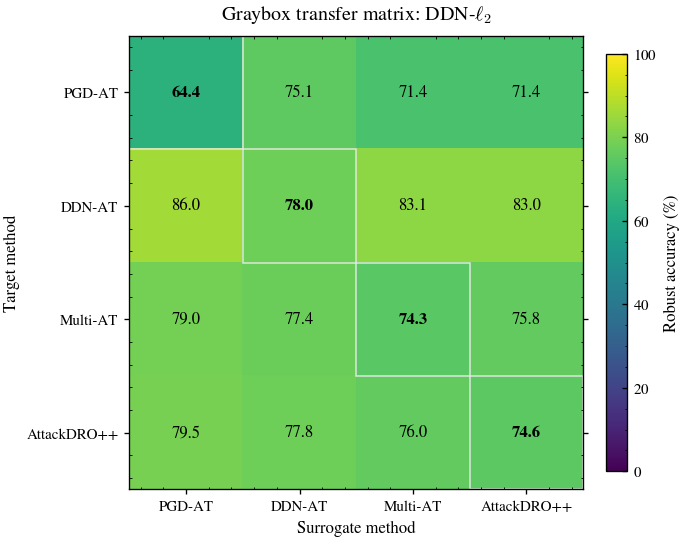
\includegraphics[width=\linewidth]{figures/graybox/transfer_matrix_4method_ddn_l2_science_clean.png}
  \\ \footnotesize (b) DDN-\(\ell_2\)
\end{minipage}

\vspace{0.6em}

\begin{minipage}{0.48\linewidth}
  \centering
  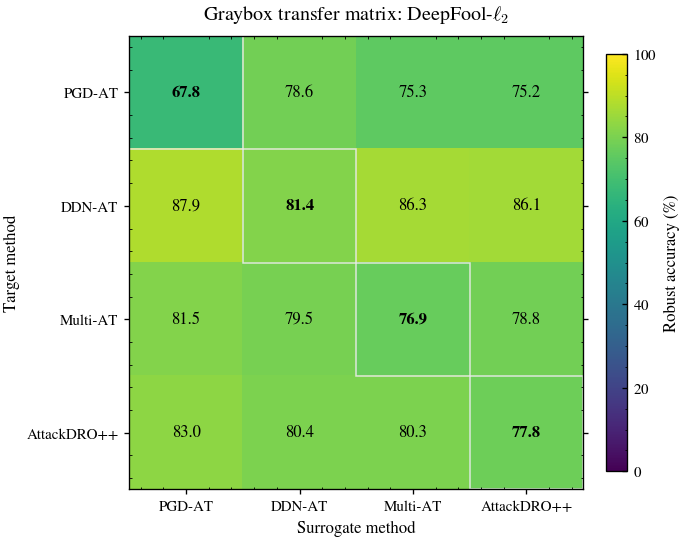
\includegraphics[width=\linewidth]{figures/graybox/transfer_matrix_4method_deepfool_l2_science_clean.png}
  \\ \footnotesize (c) DeepFool-\(\ell_2\)
\end{minipage}\hfill
\begin{minipage}{0.48\linewidth}
  \centering
  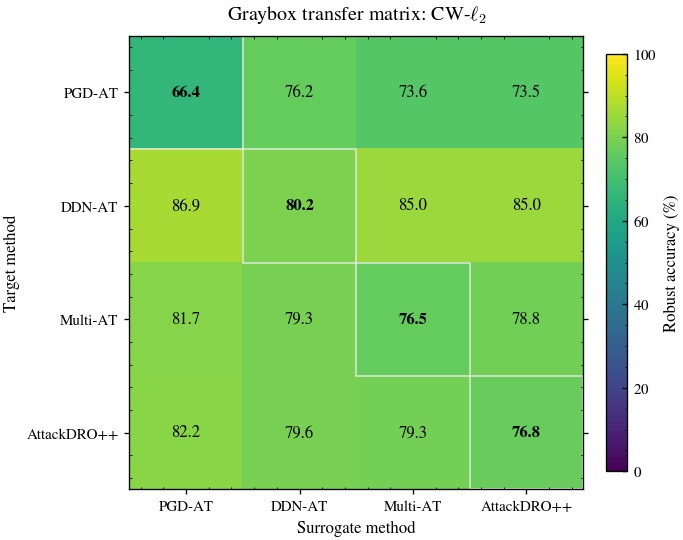
\includegraphics[width=\linewidth]{figures/graybox/transfer_matrix_4method_cw_l2_science_clean.png}
  \\ \footnotesize (d) CW-\(\ell_2\)
\end{minipage}

\caption{Per-attack graybox transfer matrices for the
\(\ell_2\)-oriented attacks. Rows are target methods and columns are
surrogate methods; cells report robust accuracy (\%).}
\label{fig:ch6_graybox_transfer_l2}
\end{figure}
On the \(\ell_2\) attacks, the DDN-AT target row is consistently strong,
especially when attacks are transferred from PGD-AT, Multi-AT, or
AttackDRO++ surrogates. This indicates that DDN-AT's high aggregate
graybox score is driven mainly by \(\ell_2\)-family transfer behavior,
rather than by uniformly strong robustness across both attack geometries.
AttackDRO++ remains closer to the balanced Multi-AT profile, while still
improving over Multi-AT on most \(\ell_2\)-oriented transfer cells.


\subsection{Paired Graybox Comparisons: Does the Whitebox Advantage Carry Over?}
\label{subsec:ch6_paired_graybox_comparisons}

% TODO[Kiệt]:
% Goal:
% - Compare AttackDRO++ against the strongest uniform multi-attack baseline under graybox transfer.
% Flow:
% - Interpret paired graybox tests, then identify where the advantage is robust or limited.
% Include:
% - Reference `tab:ch6_paired_graybox_two_panel` and `tab:ch6_graybox_attack_family`.
% Avoid:
% - Ignoring corrected p-values or effect size when discussing differences.
% Target length: 3-5 paragraphs.

The main graybox comparison is between AttackDRO++ and Multi-AT.
Both methods train on the same source attacks
$\{\text{PGD-}\ell_\infty,\ \text{DDN-}\ell_2\}$ and use the same backbone
and schedule; they differ only in the use of latent clustering, gradient
fingerprints, and the anchored Cluster-DRO objective.

We use the symmetric paired test that has already been described in
Section~\ref{sec:ch5_graybox_protocol}: for every triple
$(\text{target seed},\ \text{surrogate seed},\ \text{attack})$, we pair
the configuration ``AttackDRO++ as target, Multi-AT as surrogate'' against
its mirror ``Multi-AT as target, AttackDRO++ as surrogate'' and compute
the per-triple difference. As the results, $n = 5 \times 5 \times 8 = 200$
paired pairs make the comparison invariant to which method is chosen as
the surrogate.
\begin{table}[H]
\centering
\caption{Paired graybox comparisons. Each row uses $n=200$ paired
target--surrogate--attack triples. Positive $\Delta$ favors the reference
method named in the panel heading.}
\label{tab:ch6_paired_graybox_two_panel}
\begin{tabular}{lcccccc}
\toprule
Compared method
& \multicolumn{2}{c}{Accuracy}
& $\Delta$
& $d_z$
& $t$
& $p$ \\
\cmidrule(lr){2-3}
& Reference
& Baseline
& (pp)
& 
& 
&  \\
\midrule

\multicolumn{7}{l}{\textit{AttackDRO++ (Ours) vs. baselines}} \\
\midrule
Multi-AT
& 71.17
& 70.62
& +0.549
& 0.42
& 5.96
& \textbf{$1.1{\times}10^{-8}$} \\

PGD-AT
& 73.71
& 69.27
& \textbf{+4.435}
& 1.33
& 18.78
& \textbf{$6.1{\times}10^{-46}$} \\

DDN-AT
& 73.88
& 73.62
& +0.258
& 0.04
& 0.60
& 0.549 \\

\midrule
\multicolumn{7}{l}{\textit{Multi-AT vs. single-attack baselines}} \\
\midrule
PGD-AT
& 73.10
& 69.27
& \textbf{+3.829}
& 1.19
& 16.89
& \textbf{$2.7{\times}10^{-40}$} \\

DDN-AT
& 73.36
& 73.65
& $-0.292$
& $-0.05$
& $-0.67$
& 0.504 \\

\bottomrule
\end{tabular}
\end{table}

The AttackDRO++ vs. Multi-AT contrast is the headline result of
this section: under symmetric cross-method graybox transfer,
AttackDRO++ improves onMulti-AT by $+0.549$~pp at
$p \approx 1.1 \times 10^{-8}$, with a small-to-medium paired effect size
of $d_z \approx 0.42$. This effect is roughly twice the corresponding
whitebox delta of $+0.279$~pp on the same seed panel and is significant
at far stricter levels. The Cluster-DRO improvement therefore
\emph{strengthens} rather than disappears under graybox transfer,
indicating that the gain originates from a broader cross-attack
robustness profile rather than from a defense narrowly tuned to
AttackDRO++'s own gradients.

The single-attack contrasts confirm the expected specialist--versus--balanced
pattern. AttackDRO++ improves on PGD-AT by $+4.44$~pp at
$p < 10^{-45}$ ($d_z = 1.33$, a large effect), tracking the whitebox
trend that PGD-AT loses heavily on the $\ell_2$ family it does not train
against. The AttackDRO++ vs.\ DDN-AT contrast is statistically
indistinguishable from zero ($+0.26$~pp, $p = 0.55$); this reflects the
DDN-AT graybox inflation discussed above, not actual parity. We dissect
this asymmetry in Section~\ref{subsec:ch6_paired_graybox_comparisons}.

\paragraph{Per-attack transfer behavior.}

% TODO[Kiệt]:
% Goal:
% - Identify which attacks drive graybox transfer differences.
% Flow:
% - Discuss per-attack table, then connect attack-family behavior to whitebox findings.
% Include:
% - Reference `tab:ch6_graybox_per_attack` if retained in the main flow.
% Avoid:
% - Duplicating the transfer-matrix discussion.
% Target length: 2-4 paragraphs.

To check whether the $+0.549$~pp Mean(8) gain over Multi-AT is
broad or concentrated, we report paired graybox deltas attack by attack
on the same $n=200$ pair set. Each attack contributes $25$ paired
triples (one per surrogate--target seed combination).

\begin{table}[H]
\centering
\caption{Per-attack symmetric graybox comparison between AttackDRO++
and Multi-AT. Each attack uses \(n=25\) paired seed combinations.
Bold deltas are significant at \(p<0.05\).}
\label{tab:ch6_graybox_per_attack}
\small
\setlength{\tabcolsep}{4pt}
\renewcommand{\arraystretch}{1.10}
\begin{tabular}{llrrrr}
\toprule
Attack          & Family              & A mean (\%) & B mean (\%) & $\Delta$ (pp) & $p$ \\
\midrule
FGSM-RS         & held-out $\ell_\infty$ & $73.32$ & $72.86$ & $\mathbf{+0.454}$ & $0.0114$ \\
PGD-$\ell_\infty$ & seen $\ell_\infty$    & $57.17$ & $57.07$ & $+0.102$ & $0.307$  \\
TPGD            & held-out $\ell_\infty$ & $73.09$ & $72.30$ & $\mathbf{+0.790}$ & $0.0240$ \\
MI-FGSM         & held-out $\ell_\infty$ & $55.20$ & $54.75$ & $\mathbf{+0.458}$ & $0.0022$ \\
\midrule
PGD-$\ell_2$    & held-out $\ell_2$      & $74.97$ & $74.53$ & $\mathbf{+0.432}$ & $0.0373$ \\
DDN-$\ell_2$    & seen $\ell_2$          & $76.04$ & $75.79$ & $+0.256$ & $0.341$  \\
DeepFool-$\ell_2$ & held-out $\ell_2$    & $80.29$ & $78.82$ & $\mathbf{+1.469}$ & $0.0002$ \\
CW-$\ell_2$     & held-out $\ell_2$      & $79.26$ & $78.83$ & $+0.429$ & $0.249$  \\
\bottomrule
\end{tabular}
\end{table}

AttackDRO++ produces a positive paired delta on all eight attacks. Five
of these deltas are individually significant at $p < 0.05$, and the gain
is largest on DeepFool-$\ell_2$ ($+1.47$~pp, $p = 1.6\times 10^{-4}$),
the most local-gradient $\ell_2$ attack and the held-out attack on which
the whitebox gain over Multi-AT was also largest. The two seen
attacks (PGD-$\ell_\infty$ and DDN-$\ell_2$) contribute small,
non-significant gains, consistent with the fact that both methods
already train against these attacks. The graybox Mean(8) gain is
therefore distributed across attack families rather than concentrated on
one family.

We aggregate the per-attack deltas into the four attack groups defined
in Section~\ref{sec:ch5_evaluation_metrics} to compare the cross-method graybox
profile across all four methods.

\begin{table}[H]
\centering
\caption{Cross-method graybox accuracy by attack family. Values are
off-diagonal target accuracy (\%) averaged over the \(n=5\) panel.
Bold values mark the best method in each column.}
\label{tab:ch6_graybox_attack_family}
\small
\setlength{\tabcolsep}{6pt}
\renewcommand{\arraystretch}{1.08}
\begin{tabular}{lrrrrr}
\toprule
Target method     & Seen $\ell_\infty$ & Seen $\ell_2$ & Heldout $\ell_\infty$ & Heldout $\ell_2$ & Mean(8) \\
\midrule
PGD-AT & $\mathbf{61.48}$ & $72.61$ & $68.93$           & $74.60$           & $70.59$ \\
DDN-AT      & $56.58$          & $\mathbf{84.03}$ & $68.60$ & $\mathbf{84.85}$  & $\mathbf{75.12}$ \\
Multi-AT  & $59.71$          & $77.40$          & $68.64$ & $78.62$           & $72.36$ \\
AttackDRO++ (Ours) & $59.96$          & $77.78$          & $\mathbf{69.18}$ & $79.35$ & $72.92$ \\
\bottomrule
\end{tabular}
\end{table}

The family decomposition makes three points concrete. The held-out
$\ell_\infty$ column has AttackDRO++ at the top ($69.18\%$) by a small
but consistent margin over the other three methods. The held-out
$\ell_2$ column is dominated by DDN-AT ($84.85\%$), with AttackDRO++
($79.35\%$) ranked second and improving on Multi-AT by
$+0.73$~pp. The seen $\ell_2$ column shows the same pattern. The seen
$\ell_\infty$ column favors PGD-AT, again by structure: surrogates
generate strong PGD-$\ell_\infty$ adversarial examples, and only PGD-AT
is robust to them. AttackDRO++ is the only method that is at or above
Multi-AT on every attack family, while DDN-AT and PGD-AT each
remain narrow specialists under transfer.

\paragraph{Whitebox--graybox gap and specialist inflation.}

% TODO[Kiệt]:
% Goal:
% - Explain the gap between direct whitebox robustness and transferred robustness.
% Flow:
% - Define the gap sign, interpret `tab:ch6_graybox_gap`, then use heatmaps for method-specific patterns.
% Include:
% - Reference gap heatmaps from `fig:ch6_graybox_gap_ddnat` to `fig:ch6_graybox_gap_attackdropp`.
% - Add caption polish later for sign/unit/averaging conditions.
% Avoid:
% - Treating large whitebox scores alone as evidence of transferable robustness.
% Target length: 3-5 paragraphs.

The DDN-AT target row in Figure~\ref{fig:ch6_graybox_transfer_matrix} and
the DDN-AT row in Table~\ref{tab:ch6_graybox_attack_family} are the highest
under graybox transfer,
even though DDN-AT has the lowest whitebox Mean(8) on both the $n=5$ and
the full $n=20$ panels. We resolve this apparent contradiction by
quantifying the gap between whitebox and cross-method graybox accuracy
for each method. A large positive gap indicates that a defense looks
much stronger under graybox transfer than under direct whitebox attack,
which is a signature of a structural transfer mismatch rather than a
broader robustness profile.

\begin{table}[H]
\centering
\caption{Whitebox--graybox gap by target method on the \(n=5\) panel.
The gap is cross-method graybox Mean(8) minus diagonal whitebox Mean(8).}
\label{tab:ch6_graybox_gap}
\small
\setlength{\tabcolsep}{8pt}
\renewcommand{\arraystretch}{1.08}
\begin{tabular}{lrrr}
\toprule
Target method     & Whitebox Mean(8) & Graybox Mean(8) & Gap (pp) \\
\midrule
PGD-AT & $61.52$ & $70.59$ & $\phantom{0}+9.06$  \\
DDN-AT      & $56.92$ & $75.12$ & $\mathbf{+18.20}$   \\
Multi-AT  & $62.46$ & $72.36$ & $\phantom{0}+9.90$  \\
AttackDRO++ (Ours) & $\mathbf{62.64}$ & $72.92$ & $+10.27$   \\
\bottomrule
\end{tabular}
\end{table}

PGD-AT, Multi-AT, and AttackDRO++ all show a comparable
whitebox--graybox gap of approximately $9$--$10$~pp, indicating that
adversarial examples crafted on alternate surrogates are weaker than
those crafted directly on the target by a roughly constant amount.
DDN-AT, by contrast, gains $+18.20$~pp under graybox transfer, almost
twice the gap of any other method. Its row-leading graybox accuracy is therefore not evidence of a stronger defense; it is an artifact of
how poorly $\ell_\infty$ adversarial examples generated by PGD-AT, Multi-AT, and AttackDRO++ surrogates transfer to a
purely-$\ell_2$-trained target. AttackDRO++ retains the highest whitebox
Mean(8) of the four methods while exhibiting a graybox gap that is only
$+0.37$~pp larger than that of Multi-AT --- consistent with a
balanced cross-attack defense rather than a transfer-favored
specialist.

The per-(class \(\times\) attack) whitebox--graybox gap heatmaps in
Figures~\ref{fig:ch6_graybox_gap_ddnat}--\ref{fig:ch6_graybox_gap_attackdropp}
make the specialist-inflation effect concrete. Cell values are computed
as graybox accuracy minus whitebox accuracy, so positive values indicate
that transferred attacks are weaker than direct whitebox attacks on the
same target.

\begin{figure}[H]
\centering
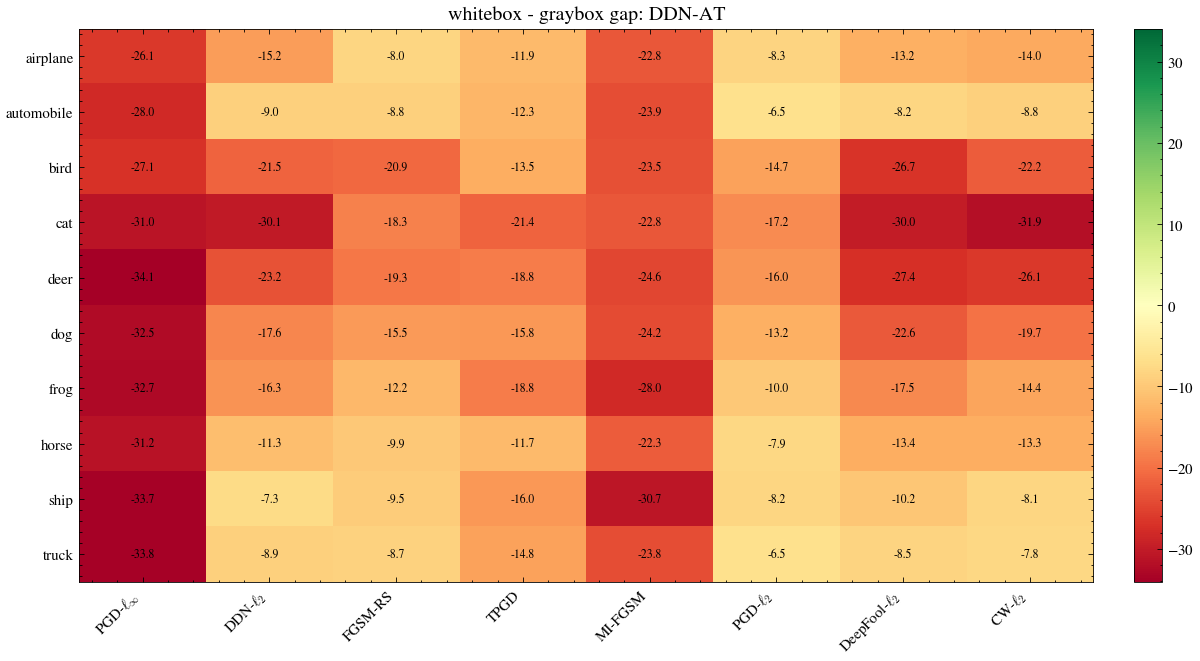
\includegraphics[width=\linewidth]{figures/graybox/whitebox_graybox_gap_DDNAT.png}
\caption{Whitebox--graybox gap heatmap for DDN-AT.}
\label{fig:ch6_graybox_gap_ddnat}
\end{figure}

\begin{figure}[H]
\centering
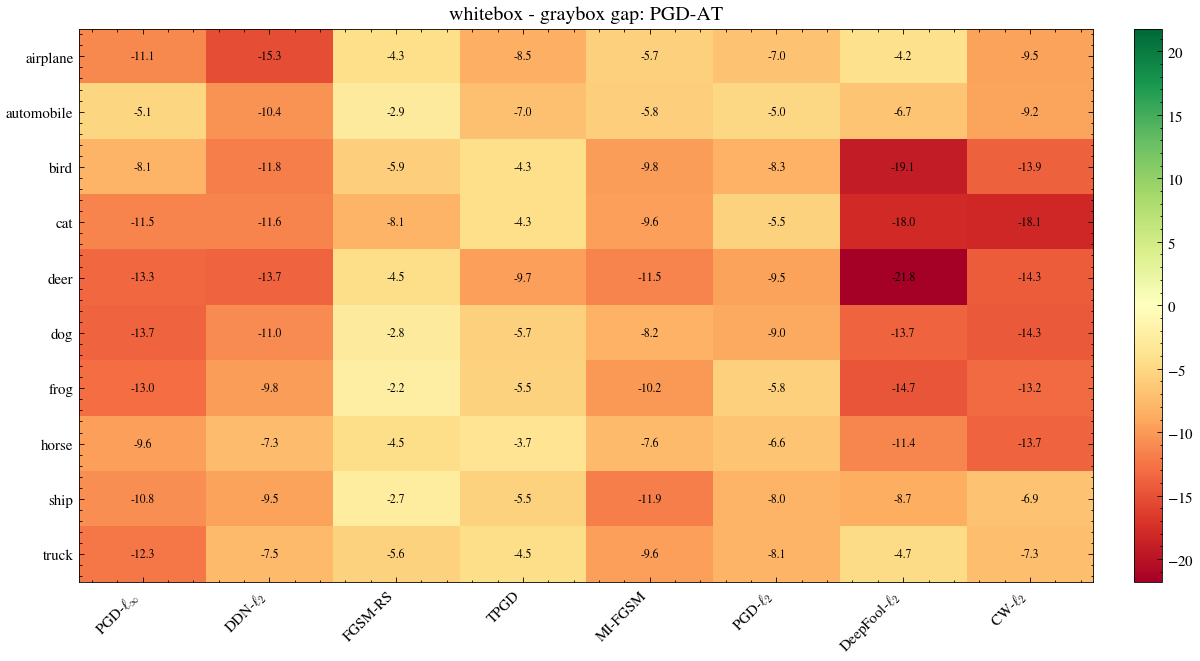
\includegraphics[width=\linewidth]{figures/graybox/whitebox_graybox_gap_PGDAT.png}
\caption{Whitebox--graybox gap heatmap for PGD-AT.}
\label{fig:ch6_graybox_gap_pgdat}
\end{figure}

\begin{figure}[H]
\centering
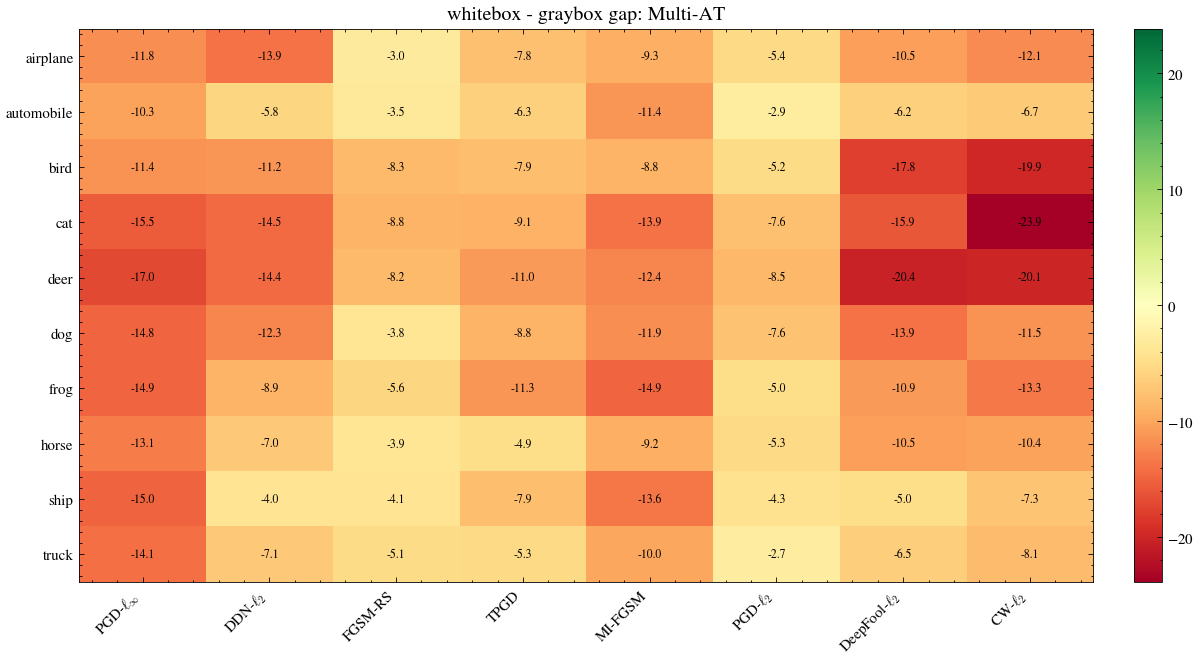
\includegraphics[width=\linewidth]{figures/graybox/whitebox_graybox_gap_MultiAT.png}
\caption{Whitebox--graybox gap heatmap for Multi-AT.}
\label{fig:ch6_graybox_gap_multiat}
\end{figure}

\begin{figure}[H]
\centering
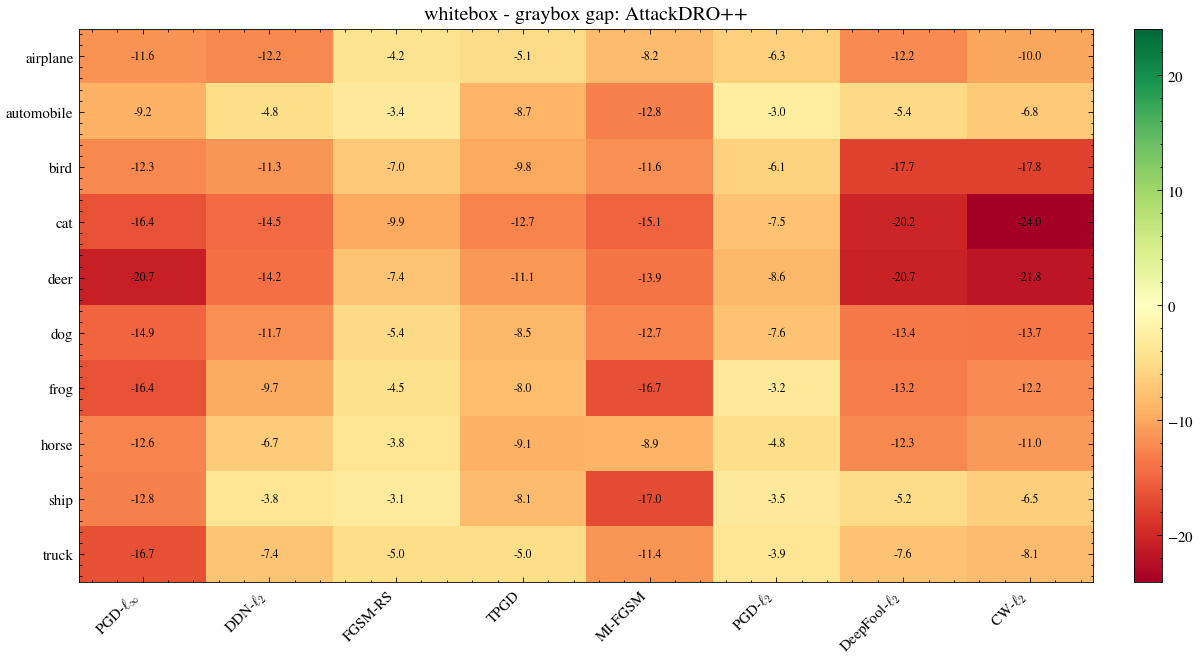
\includegraphics[width=\linewidth]{figures/graybox/whitebox_graybox_gap_AttackDROpp.png}
\caption{Whitebox--graybox gap heatmap for AttackDRO++ (Ours).}
\label{fig:ch6_graybox_gap_attackdropp}
\end{figure}

DDN-AT exhibits broad positive gaps on the \(\ell_\infty\)-oriented
attack columns, indicating that its high graybox score is partly driven
by weak transfer from \(\ell_\infty\) surrogates rather than uniformly
strong robustness. PGD-AT, Multi-AT, and AttackDRO++ show smaller and
more balanced gap patterns, with AttackDRO++ avoiding the severe
specialist inflation observed for DDN-AT.
\subsection{Class-Level Transfer Patterns}
\label{subsec:ch6_class_level_transfer_patterns}

% TODO[Kiệt]:
% Goal:
% - Explain fine-grained graybox gains and failures by class and attack.
% Flow:
% - Interpret `tab:ch6_graybox_per_cell`, then use delta heatmaps to show where gains concentrate.
% Include:
% - Reference `fig:ch6_graybox_delta_multiat`, `fig:ch6_graybox_delta_pgdat`, and `fig:ch6_graybox_delta_ddnat` if all remain in the main flow.
% Avoid:
% - Listing every class-attack cell.
% Target length: 3-5 paragraphs.

We complement the aggregate analysis with a paired per-cell test. For
each of the $80$ attack--class cells, we compare the graybox accuracy of
the AttackDRO++ target against each baseline target across the five
training seeds (each cell pairs $n = 5$ seeds). A two-sided paired
$t$-test is computed per cell.

\begin{table}[H]
\centering
\caption{Per-(class \(\times\) attack) graybox tests comparing
AttackDRO++ against each baseline. \(\Delta\) is computed as
AttackDRO++ minus the baseline.}
\label{tab:ch6_graybox_per_cell}
\footnotesize
\setlength{\tabcolsep}{4.5pt}
\renewcommand{\arraystretch}{1.18}
\begin{tabular}{lccccc}
\toprule
Baseline
& Positive cells
& Sign-test
& Mean
& Significant cells
& Bottom-10 \\
& \((\Delta>0)\)
& \(p\)
& \(\Delta\) (pp)
& AttackDRO++ / Baseline
& lift (pp) \\
\midrule
Multi-AT
& $59/80$
& $\mathbf{1.3{\times}10^{-5}}$
& $+0.557$
& $\phantom{0}2 \,/\, \phantom{0}3$
& $+0.779$ \\

PGD-AT
& $52/80$
& $\mathbf{4.8{\times}10^{-3}}$
& $+2.332$
& $34 \,/\, 12$
& $+1.329$ \\

DDN-AT
& $27/80$
& $\mathbf{2.4{\times}10^{-3}}$
& $-2.206$
& $16 \,/\, 32$
& $+0.709$ \\
\bottomrule
\end{tabular}
\end{table}

Three observations follow. First, AttackDRO++ exceeds Multi-AT on
$59$ of $80$ cells with a mean per-cell delta of $+0.557$~pp, in close
agreement with the $+0.549$~pp aggregate from
Table~\ref{tab:ch6_paired_graybox_two_panel}. Cell-level significance is sparse
($2$ vs.\ $3$ cells reach $p < 0.05$ in either direction), as expected
under the $n = 5$ per-cell sample size and the small absolute deltas;
the bulk of the evidence for AttackDRO++ is therefore the
\emph{distributional} shift across many cells rather than a few cell-level
landslides.

Second, the bottom-10 lift is positive in all three contrasts. The cells
on which Multi-AT, PGD-AT, and DDN-AT are weakest concentrate on
the cat, deer, dog, and bird classes under MI-FGSM, PGD-$\ell_\infty$,
and PGD-$\ell_2$. AttackDRO++ improves on Multi-AT by
$+0.779$~pp on Multi-AT's worst $10$ cells, and improves on
PGD-AT by $+1.329$~pp on PGD-AT's worst $10$ cells.

Third, the AttackDRO++ vs.\ DDN-AT cell-level comparison ($-2.21$~pp on
average, $32$ cells favoring DDN-AT at $p<0.05$) is the per-cell
counterpart of the DDN-AT graybox inflation: most of DDN-AT's wins are
on $\ell_2$ cells, while AttackDRO++ retains the wins it needs on the
$\ell_\infty$ cells that DDN-AT collapses on under whitebox attack
(Section~\ref{subsec:ch6_per_attack_accuracy}).

The heatmaps in
Figures~\ref{fig:ch6_graybox_delta_multiat}--\ref{fig:ch6_graybox_delta_ddnat} visualize these patterns
explicitly: green cells favor AttackDRO++, red cells favor the baseline.
The AttackDRO++ vs.\ Multi-AT heatmap is broadly green and small
in magnitude; the AttackDRO++ vs.\ PGD-AT heatmap is broadly green with
a few large red cells on $\ell_\infty$ attacks where PGD-AT specializes;
and the AttackDRO++ vs.\ DDN-AT heatmap is mixed.

\begin{figure}[H]
\centering
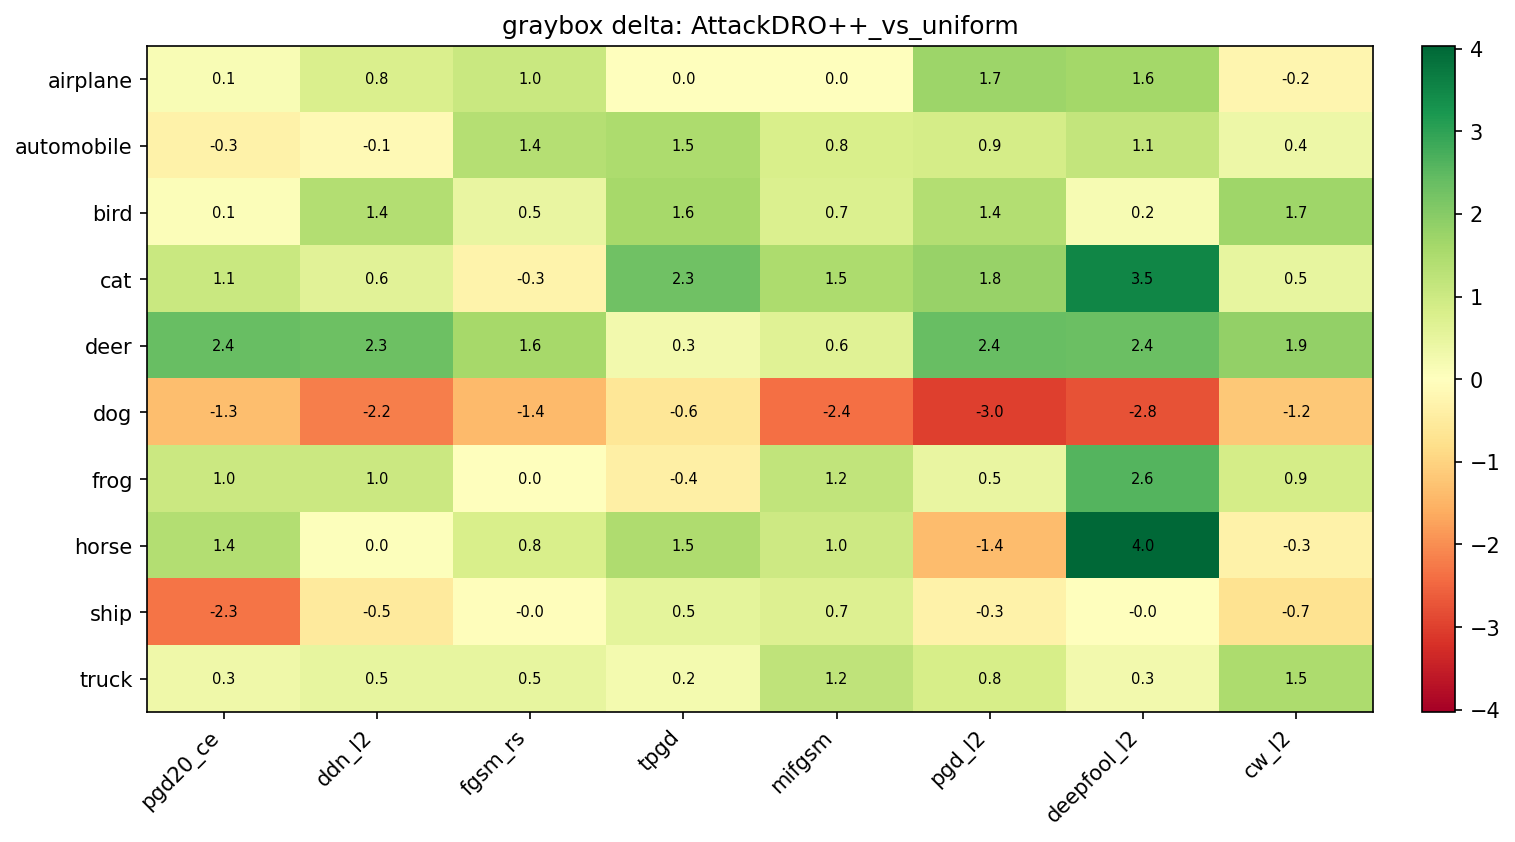
\includegraphics[width=\linewidth]{figures/graybox/graybox_delta_per_class_attack_AttackDRO++_vs_uniform.png}
\caption{Per-(class \(\times\) attack) graybox delta heatmap for
AttackDRO++ (Ours) minus Multi-AT. Green favors AttackDRO++ (Ours); red favors
Multi-AT.}
\label{fig:ch6_graybox_delta_multiat}
\end{figure}

\begin{figure}[H]
\centering
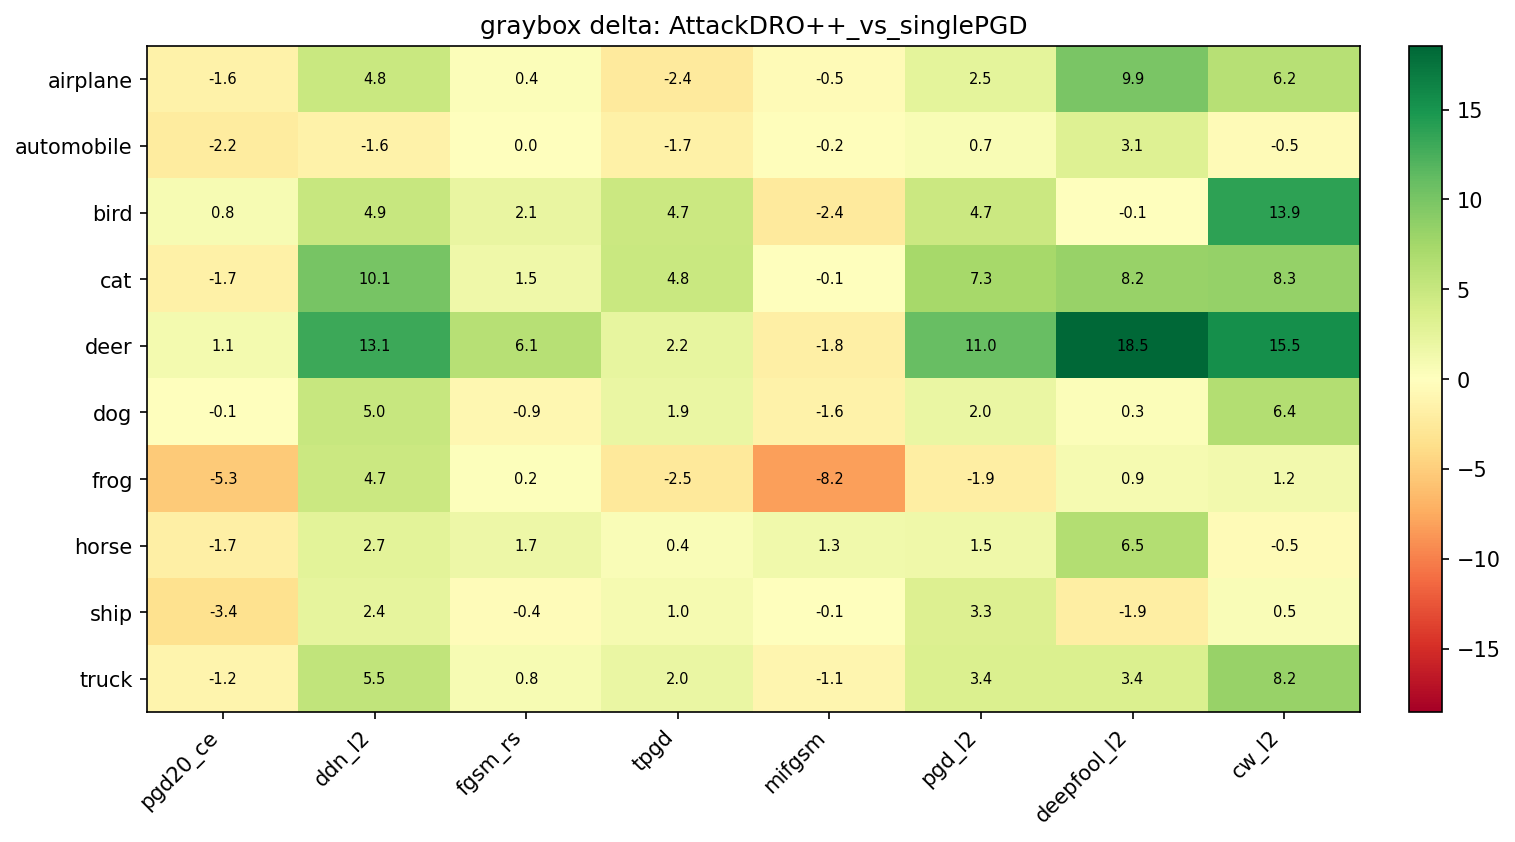
\includegraphics[width=\linewidth]{figures/graybox/graybox_delta_per_class_attack_AttackDRO++_vs_singlePGD.png}
\caption{Per-(class \(\times\) attack) graybox delta heatmap for
AttackDRO++ (Ours) minus PGD-AT. Green favors AttackDRO++ (Ours); red favors PGD-AT.}
\label{fig:ch6_graybox_delta_pgdat}
\end{figure}

\begin{figure}[H]
\centering
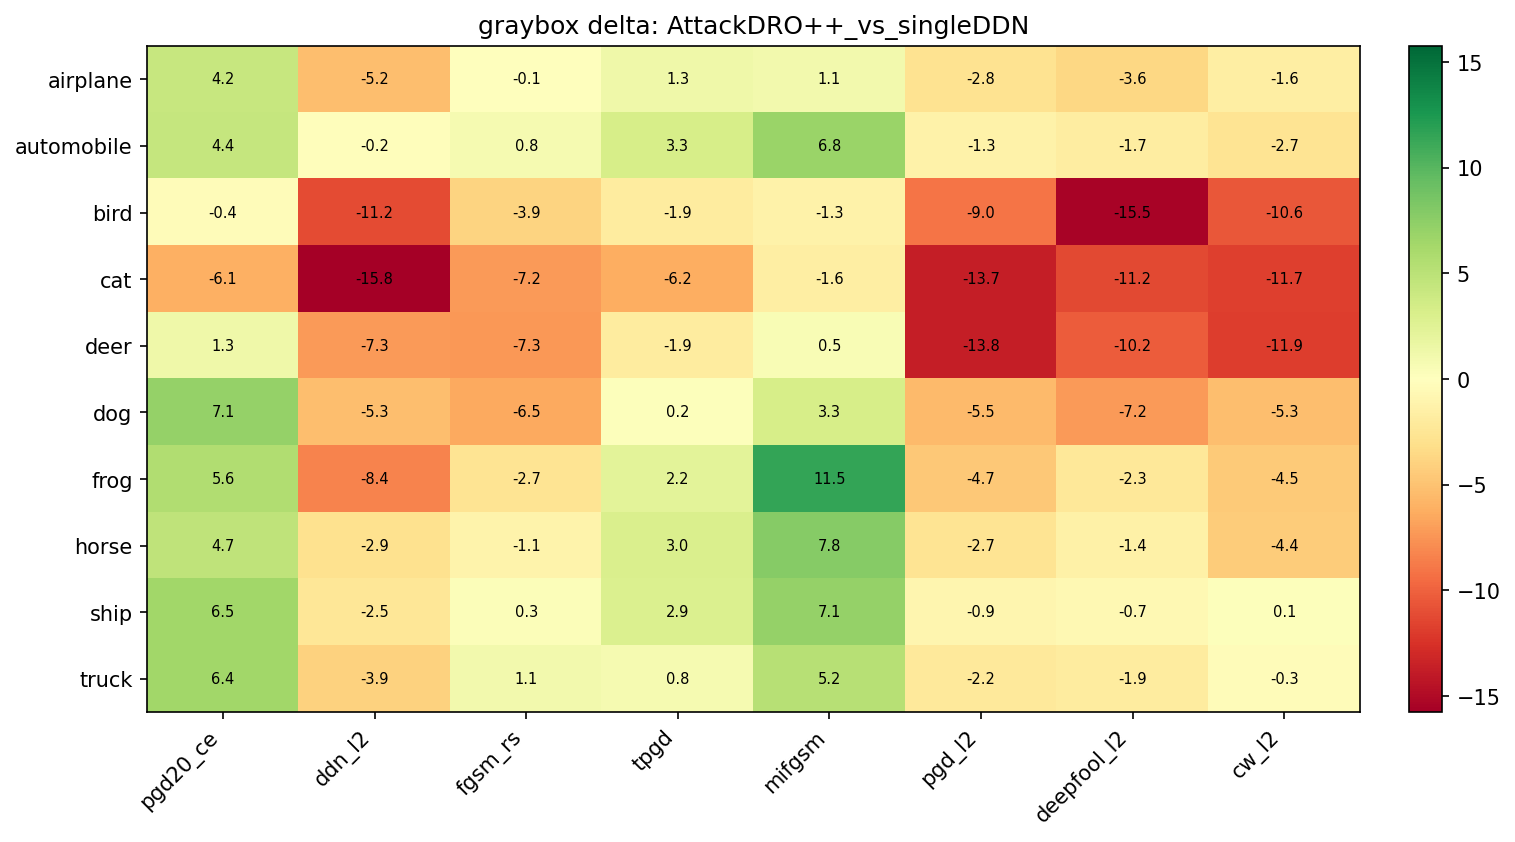
\includegraphics[width=\linewidth]{figures/graybox/graybox_delta_per_class_attack_AttackDRO++_vs_singleDDN.png}
\caption{Per-(class \(\times\) attack) graybox delta heatmap for
AttackDRO++ (Ours) minus DDN-AT. Green favors AttackDRO++ (Ours); red favors DDN-AT.}
\label{fig:ch6_graybox_delta_ddnat}
\end{figure}

\newpage
\paragraph{Method contribution decomposition.}

% TODO[Kiệt]:
% Goal:
% - Explain the contribution split between multi-attack training and Cluster-DRO components.
% Flow:
% - Interpret the decomposition table first, then use the figure as visual support.
% Include:
% - Reference `tab:ch6_graybox_decomposition` and `fig:ch6_method_decomposition` if kept.
% Avoid:
% - Treating decomposition as causal proof beyond the available comparisons.
% Target length: 2-4 paragraphs.

The whitebox results of Section~\ref{sec:ch6_whitebox} compare AttackDRO++
against Multi-AT and against the two single-attack baselines as
three separate contrasts. Under graybox transfer, we can additionally
ask how much of the AttackDRO++ improvement over each single-attack
baseline is contributed by multi-attack training (the Multi-AT
component) versus the Cluster-DRO objective (the AttackDRO++ component
on top of Multi-AT). We decompose the total
AttackDRO++ vs.\ single-attack delta as
\[
\Delta_{\text{total}}
\;=\;
\underbrace{(\text{Multi-AT}) - (\text{single-AT})}_{\Delta_{\text{multi-attack}}}
\;+\;
\underbrace{(\text{AttackDRO++}) - (\text{Multi-AT})}_{\Delta_{\text{Cluster-DRO}}},
\]
and report this decomposition for whitebox Mean(8), cross-method graybox
Mean(8), and the bottom-10-cell cross-method graybox average (the average
graybox accuracy on the ten attack--class cells in which the target is
weakest). The bottom-10 metric is included because it isolates worst-cell
behavior, which is most sensitive to the AttackDRO++ objective.

\begin{table}[H]
\centering
\caption{AttackDRO++ (Ours) gain decomposition. Values are percentage-point changes.}
\label{tab:ch6_graybox_decomposition}
\small
\setlength{\tabcolsep}{6pt}
\renewcommand{\arraystretch}{1.10}
\begin{tabular}{llrrr}
\toprule
Metric & Base & Multi-AT & DRO++ & Total \\
\midrule
Whitebox Mean(8)        & PGD-AT & $+0.934$ & $+0.184$ & $+1.118$ \\
Whitebox Mean(8)        & DDN-AT & $+5.536$ & $+0.184$ & $+5.720$ \\
\midrule
Cross-graybox Mean(8)   & PGD-AT & $+1.775$ & $+0.557$ & $+2.332$ \\
Cross-graybox Mean(8)   & DDN-AT & $-2.763$ & $+0.557$ & $-2.206$ \\
\midrule
Bottom-10 graybox       & PGD-AT & $+0.530$ & $+0.799$ & $+1.329$ \\
Bottom-10 graybox       & DDN-AT & $-0.090$ & $+0.799$ & $+0.709$ \\
\bottomrule
\end{tabular}
\end{table}
The Cluster-DRO effect (column 4) is positive on every metric and
decomposition path, ranging from $+0.184$~pp on whitebox Mean(8) to
$+0.799$~pp on the bottom-10 cross-graybox metric. Two implications
follow. First, the Cluster-DRO effect is larger under graybox transfer
than under direct whitebox attack, consistent with the
$+0.279$~pp $\rightarrow$ $+0.549$~pp scaling observed in
Section~\ref{subsec:ch6_paired_graybox_comparisons}. Second, the Cluster-DRO effect is
roughly four times larger on the bottom-10 cells ($+0.799$~pp) than on
whitebox Mean(8), supporting the design intent that the Cluster-DRO
objective primarily reshapes worst-cell behavior rather than the
average.

The multi-attack column tells a complementary specialist story. Going
from single-AT to Multi-AT adds $+5.54$~pp of whitebox Mean(8)
when the baseline is DDN-AT, but removes $-2.76$~pp of cross-graybox
Mean(8) for the same baseline --- because DDN-AT's graybox accuracy is
inflated by the very $\ell_\infty$ transfer mismatch that
Multi-AT corrects. The cluster-DRO component remains positive in both
cases, indicating that it adds robustness that is not absorbed by either
multi-attack training alone or DDN-AT's structural graybox advantage.

\begin{figure}[H]
\centering
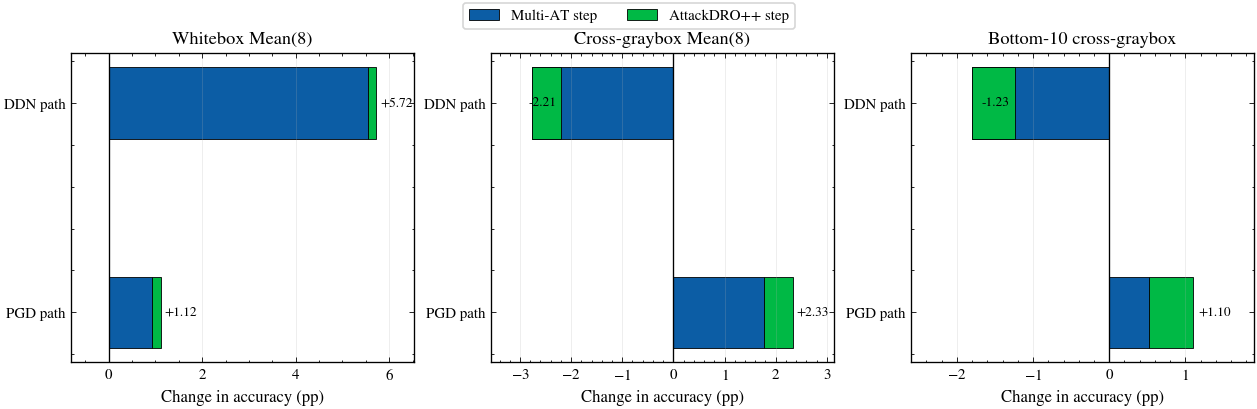
\includegraphics[width=\linewidth]{figures/graybox/method_decomposition_three_panel_science.png}
\caption{Visual decomposition of AttackDRO++ improvement over the
single-attack baselines into a multi-attack effect (Multi-AT
minus single-AT) and a Cluster-DRO effect (AttackDRO++ minus Multi-AT) across whitebox, cross-method graybox, and bottom-10
cross-method graybox metrics, for the two single-AT decomposition
paths.}
\label{fig:ch6_method_decomposition}
\end{figure}

% Section summary removed; transition/closing prose should be written later.
\iffalse
% Disabled graybox section summary removed from the numbered structure.

% TODO[Kiệt]:
% Goal:
% - Remove or convert this section-level summary in a later style cleanup.
% Flow:
% - Replace with a short transition paragraph or move synthesis into `6_summary.tex`.
% Include:
% - No new results.
% Avoid:
% - Keeping section-level summaries against docs/06_style_rules.md.
% Target length: 0 paragraphs here after cleanup; use Chapter 6 summary instead.

The graybox transfer results jointly establish the following
conclusions:

\begin{enumerate}
  \item The graybox random-seed checkpoint panel preserves the whitebox
        trend: it reproduces the Mean(8) ranking AttackDRO++ $>$ Multi-AT
        $>$ PGD-AT $>$ DDN-AT to within $1.0$~pp.
  \item AttackDRO++ improves on Multi-AT by $+0.549$~pp under
        symmetric cross-method graybox transfer at $p \approx 1.1
        \times 10^{-8}$ ($d_z = 0.42$, $n=200$), roughly twice the
        whitebox delta on the same panel. The Cluster-DRO improvement
        therefore strengthens rather than disappears under transfer.
  \item The graybox gain is broad: AttackDRO++ produces a positive
        per-attack delta against Multi-AT on all eight
        evaluation attacks, with five attacks individually significant
        at $p<0.05$ and the largest gain on DeepFool-$\ell_2$
        ($+1.47$~pp, $p<10^{-3}$). It is the only method that meets or
        exceeds Multi-AT on every attack family.
  \item DDN-AT's row-leading graybox accuracy is structural rather
        than substantive.. Its whitebox--graybox gap is $+18.20$~pp,
        roughly twice that of every other method, because $\ell_\infty$
        adversarial examples generated by alternative surrogates
        transfer poorly to a purely-$\ell_2$-trained target. The strong
        graybox row should not be confused with broader robustness;
        DDN-AT's whitebox Mean(8) and Worst(8) remain the lowest of
        the four methods.
  \item The per-cell drilldown shows that AttackDRO++ exceeds        Multi-AT on $59$ of $80$ attack--class cells, with a bottom-10
        lift of $+0.779$~pp on Multi-AT's weakest cells. The
        Cluster-DRO contribution decomposes as approximately $+0.18$~pp
        on whitebox Mean(8), $+0.56$~pp on cross-graybox Mean(8), and
        $+0.80$~pp on the bottom-10 cross-graybox metric, supporting
        the design intent that the objective primarily reshapes
        worst-cell behavior.
\end{enumerate}

These graybox results corroborate the whitebox conclusions of
Section~\ref{sec:ch6_whitebox}: the AttackDRO++ improvement over
Multi-AT reflects a broader cross-attack robustness profile, not a
defense narrowly tuned to its own gradients. The single-attack baselines
remain specialists under both whitebox and graybox attack, and DDN-AT's
apparent graybox strength is exposed as a transfer-mismatch artefact by
the whitebox--graybox gap analysis. The next section examines how these
behaviors emerge during training.
\fi

\section{Sensitivity to Key Hyperparameters}
\label{sec:ch6_ablation}

The preceding sections evaluated the final AttackDRO++ configuration under
whitebox, class-wise, and graybox settings. Those results show how the method
behaves once the design choices are fixed, but they do not explain how sensitive
the method is to those choices. This section therefore studies three practical
hyperparameters: the number of discovered clusters, the strength of the uniform
anchor, and the frequency with which clusters are refreshed.

These ablations are intended as configuration guidance rather than as a second
main comparison. Unless otherwise stated, they use the same CIFAR-10, ResNet-18,
source-attack, and evaluation-attack protocol defined in Chapter~\ref{chap:experimental_setup}.
Mean(8) and Worst(8) follow the definitions in Section~\ref{sec:ch5_evaluation_metrics}:
both are computed over the eight non-AutoAttack evaluation attacks, while
AutoAttack-$\ell_\infty$ is reported separately.

\subsection{Number of Clusters: How Many Groups Are Needed?}
\label{subsec:ch6_ablation_num_clusters}

The number of clusters controls the granularity of the latent groups used by
AttackDRO++. If $K$ is too small, distinct failure modes may be merged into the
same group, making the Cluster-DRO correction too coarse. If $K$ is too large,
the minibatch may be split into many small groups, making group-loss estimates
noisier and the cluster weights less stable.

Because $K$ controls the trade-off between coarse grouping and noisy small groups,
Table~\ref{tab:ch6_ablation_num_clusters} tests whether AttackDRO++ is sensitive to
cluster granularity. Across the available runs, all settings remain close in Mean(8), with differences
well below one percentage point. The default $K=4$ setting gives the highest
Worst(8) among the tested settings and remains competitive in Mean(8), while
$K=2$ is slightly more coarse and $K=6$ or $K=10$ do not provide a clear gain.
The $K=10$ setting uses only two valid runs and should be interpreted
as weaker evidence than the other cluster-count settings.

\begin{table}[H]
\centering
\caption{Number-of-clusters ablation for AttackDRO++ with anchor strength
$\lambda_{\mathrm{DRO}}=0.35$. Values are robust accuracy (\%) reported as
mean $\pm$ standard deviation across available runs. Mean(8) and Worst(8) are
computed over the eight non-AutoAttack attacks; AutoAttack-$\ell_\infty$ is
reported separately. Bold values indicate the best setting for each metric.}
\label{tab:ch6_ablation_num_clusters}
\small
\setlength{\tabcolsep}{4pt}
\renewcommand{\arraystretch}{1.08}
\begin{tabular}{lccccc}
\toprule
Setting & $K$ & Runs & Mean(8) $\uparrow$ & Worst(8) $\uparrow$ & AutoAttack $\uparrow$ \\
\midrule
Coarse grouping
& 2 & 3
& $62.33 \pm 0.06$
& $45.13 \pm 0.27$
& $40.95 \pm 0.90$ \\

Default grouping
& 4 & 3
& \bestval{62.35 $\pm$ 0.20}
& \bestval{45.33 $\pm$ 0.25}
& \bestval{41.14 $\pm$ 1.15} \\

Finer grouping
& 6 & 3
& $62.28 \pm 0.14$
& $45.17 \pm 0.47$
& $40.95 \pm 1.30$ \\

Very fine grouping
& 10 & 2
& $62.35 \pm 0.09$
& $45.17 \pm 0.08$
& $40.62 \pm 1.11$ \\
\bottomrule
\end{tabular}
\end{table}

\begin{figure}[H]
    \centering
    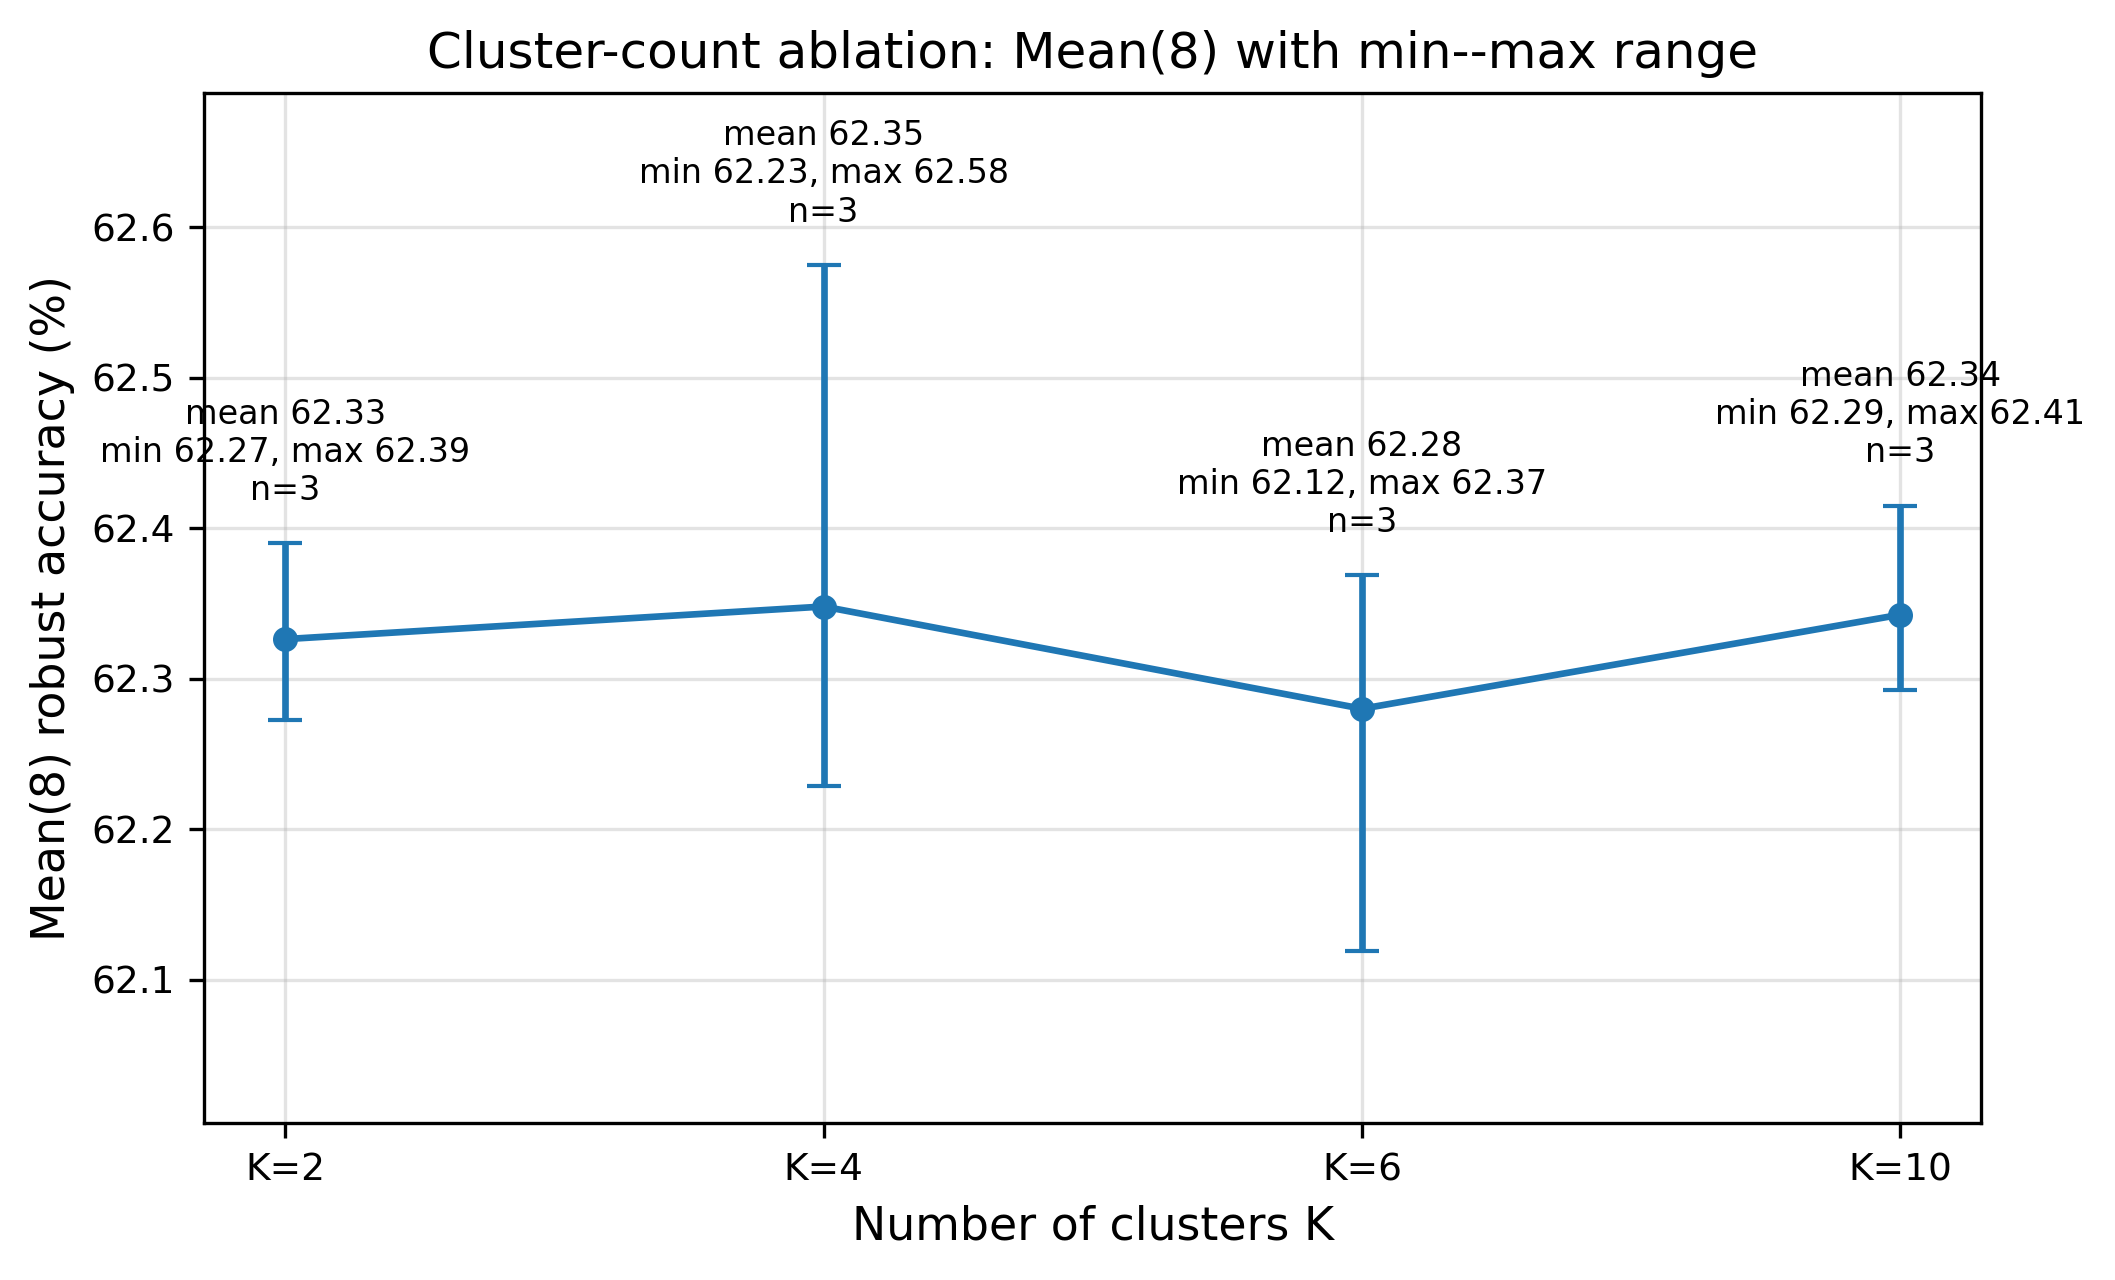
\includegraphics[width=0.82\linewidth]{figures/ablations/ablation_num_clusters.png}
    \caption{Sensitivity of AttackDRO++ to the number of clusters. Points show Mean(8) robust accuracy with the min-to-max range across available runs; Mean(8) is computed over the eight non-AutoAttack evaluation attacks.}
    \label{fig:ch6_ablation_num_clusters}
\end{figure}

The ablation supports using a moderate number of clusters rather than treating
the cluster count as a highly tuned parameter. The default $K=4$ is expressive
enough to go beyond the two source attack identities, but it does not fragment
the training batch as aggressively as larger values. Therefore, the evidence
supports $K=4$ as a stable practical choice, not as a universally optimal cluster
count.

\subsection{Anchor Strength: Finding a Stable Trade-off}
\label{subsec:ch6_ablation_anchor_strength}

The anchor strength $\lambda_{\mathrm{DRO}}$ controls the interpolation between
the uniform multi-attack ERM objective and the adaptive Cluster-DRO objective.
A smaller value keeps training closer to the uniform baseline, while a larger
value gives the cluster-reweighted loss more influence. In this ablation, the
previous $\lambda_{\mathrm{DRO}}=1.0$ setting is removed because it corresponds
to an overly aggressive Cluster-DRO setting and is not part of the final
candidate set.

Because the anchor controls how far the objective can move away from uniform Multi-AT,
Table~\ref{tab:ch6_ablation_anchor_strength} tests three practical anchor strengths.
The differences are again small, but the moderate setting
$\lambda_{\mathrm{DRO}}=0.35$ gives the strongest Mean(8), Worst(8), and
AutoAttack values among the tested settings. The lower value
$\lambda_{\mathrm{DRO}}=0.20$ remains close, suggesting that the method does not
require a sharply tuned anchor. The higher value $\lambda_{\mathrm{DRO}}=0.50$
slightly reduces Mean(8) and AutoAttack, which is consistent with the idea that
too much emphasis on adaptive cluster weighting can reduce the stabilizing effect
of the uniform multi-attack baseline.

\begin{table}[H]
\centering
\caption{Anchor-strength ablation for AttackDRO++ with $K=4$. Values are robust
accuracy (\%) reported as mean $\pm$ standard deviation across three runs.
Mean(8) and Worst(8) are computed over the eight non-AutoAttack attacks;
AutoAttack-$\ell_\infty$ is reported separately. Bold values indicate the best setting for each metric.}
\label{tab:ch6_ablation_anchor_strength}
\small
\setlength{\tabcolsep}{4pt}
\renewcommand{\arraystretch}{1.08}
\begin{tabular}{lcccc}
\toprule
Anchor strength $\lambda_{\mathrm{DRO}}$ & Runs & Mean(8) $\uparrow$ & Worst(8) $\uparrow$ & AutoAttack $\uparrow$ \\
\midrule
$0.20$
& 3
& $62.28 \pm 0.09$
& $45.01 \pm 0.40$
& $41.08 \pm 1.66$ \\

$0.35$ (default)
& 3
& \bestval{62.35 $\pm$ 0.20}
& \bestval{45.33 $\pm$ 0.25}
& \bestval{41.14 $\pm$ 1.15} \\

$0.50$
& 3
& $62.24 \pm 0.18$
& $45.24 \pm 0.40$
& $40.24 \pm 1.09$ \\
\bottomrule
\end{tabular}
\end{table}

\begin{figure}[H]
    \centering
    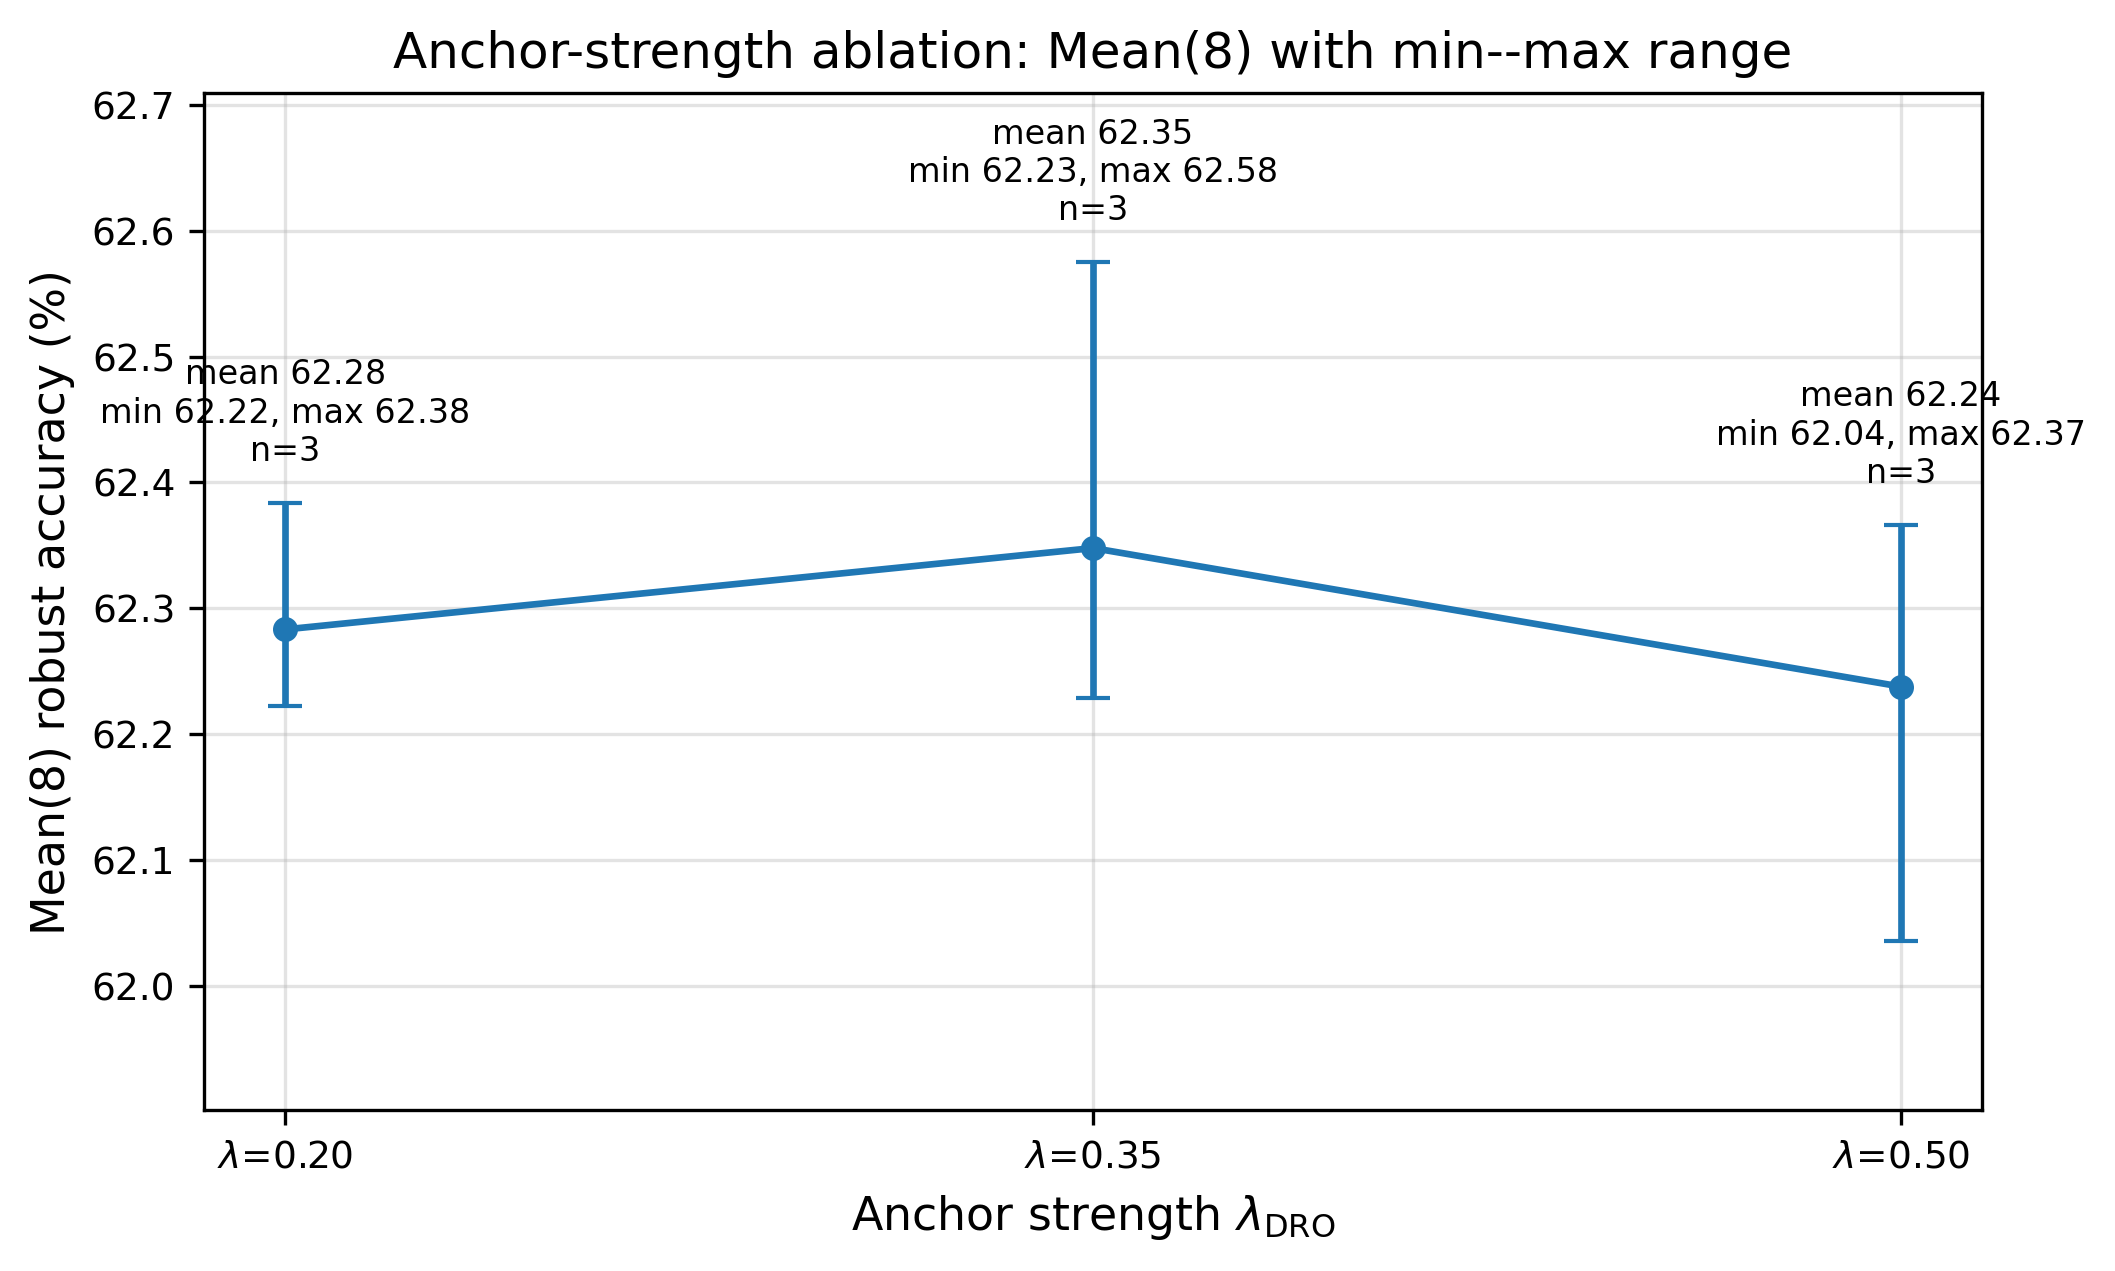
\includegraphics[width=0.82\linewidth]{figures/ablations/ablation_anchor_strength.png}
    \caption{Sensitivity of AttackDRO++ to the anchor strength $\lambda_{\mathrm{DRO}}$. Points show Mean(8) robust accuracy with the min-to-max range across available runs; Mean(8) is computed over the eight non-AutoAttack evaluation attacks. The previous $\lambda_{\mathrm{DRO}}=1.0$ setting is excluded from the final ablation panel.}
    \label{fig:ch6_ablation_anchor_strength}
\end{figure}

Overall, the anchor-strength ablation supports the design motivation from
Chapter~\ref{chap:methodology}. AttackDRO++ benefits from a nonzero
cluster-level correction, but the correction should remain anchored to the
uniform multi-attack objective. The default value
$\lambda_{\mathrm{DRO}}=0.35$ is retained because it gives the best balance
among the tested settings without relying entirely on either uniform ERM or
aggressive Cluster-DRO weighting.

\subsection{Recluster Frequency: How Often Should Groups Update?}
\label{subsec:ch6_ablation_recluster_frequency}

The cluster-refresh interval $R$ controls how often the K-means clusterer is
refitted from the feature bank. Refreshing every epoch may adapt faster to
changes in the representation, but it also changes the group structure more
frequently. Refreshing less often may give a more stable grouping signal, but it
may lag behind the evolving model.

Since the refresh interval trades adaptation speed against group stability,
Table~\ref{tab:ch6_cluster_refresh_schedule_ablation} compares refreshing every
one epoch with refreshing every two epochs. The two schedules produce nearly
identical Mean(8), Worst(8), and family-level behavior. The default two-epoch
schedule gives a slightly higher Mean(8) and $\ell_\infty$-family average, while
the one-epoch schedule gives a slightly higher Worst(8), AutoAttack, and
$\ell_2$-family average. These differences are small relative to the
three-run setting, so the ablation does not show a strong advantage for either
schedule.

\begin{table}[H]
\centering
\caption{Cluster-refresh schedule ablation for AttackDRO++ with
$\lambda_{\mathrm{DRO}}=0.35$, gradient fingerprints, and $K=4$. Values are
robust accuracy (\%) reported as mean $\pm$ standard deviation across three
runs. Mean(8) and Worst(8) are computed over the eight non-AutoAttack attacks;
AutoAttack-$\ell_\infty$ is reported separately. Bold values indicate the best setting for each metric.}
\label{tab:ch6_cluster_refresh_schedule_ablation}
\scriptsize
\setlength{\tabcolsep}{4pt}
\renewcommand{\arraystretch}{1.08}
\resizebox{\textwidth}{!}{%
\begin{tabular}{lcccccc}
\toprule
Refresh interval
& Runs
& Mean(8) $\uparrow$
& Worst(8) $\uparrow$
& AutoAttack $\uparrow$
& $\ell_2$-family avg. $\uparrow$
& $\ell_\infty$-family avg. $\uparrow$ \\
\midrule
1 epoch
& 3
& $62.38 \pm 0.14$
& \bestval{45.17 $\pm$ 0.34}
& \bestval{40.30 $\pm$ 1.37}
& \bestval{67.57 $\pm$ 0.16}
& $57.18 \pm 0.27$ \\

2 epochs (default)
& 3
& \bestval{62.44 $\pm$ 0.22}
& $45.14 \pm 0.23$
& $39.45 \pm 0.68$
& $67.56 \pm 0.08$
& \bestval{57.31 $\pm$ 0.35} \\
\bottomrule
\end{tabular}}
\end{table}

\begin{figure}[H]
    \centering
    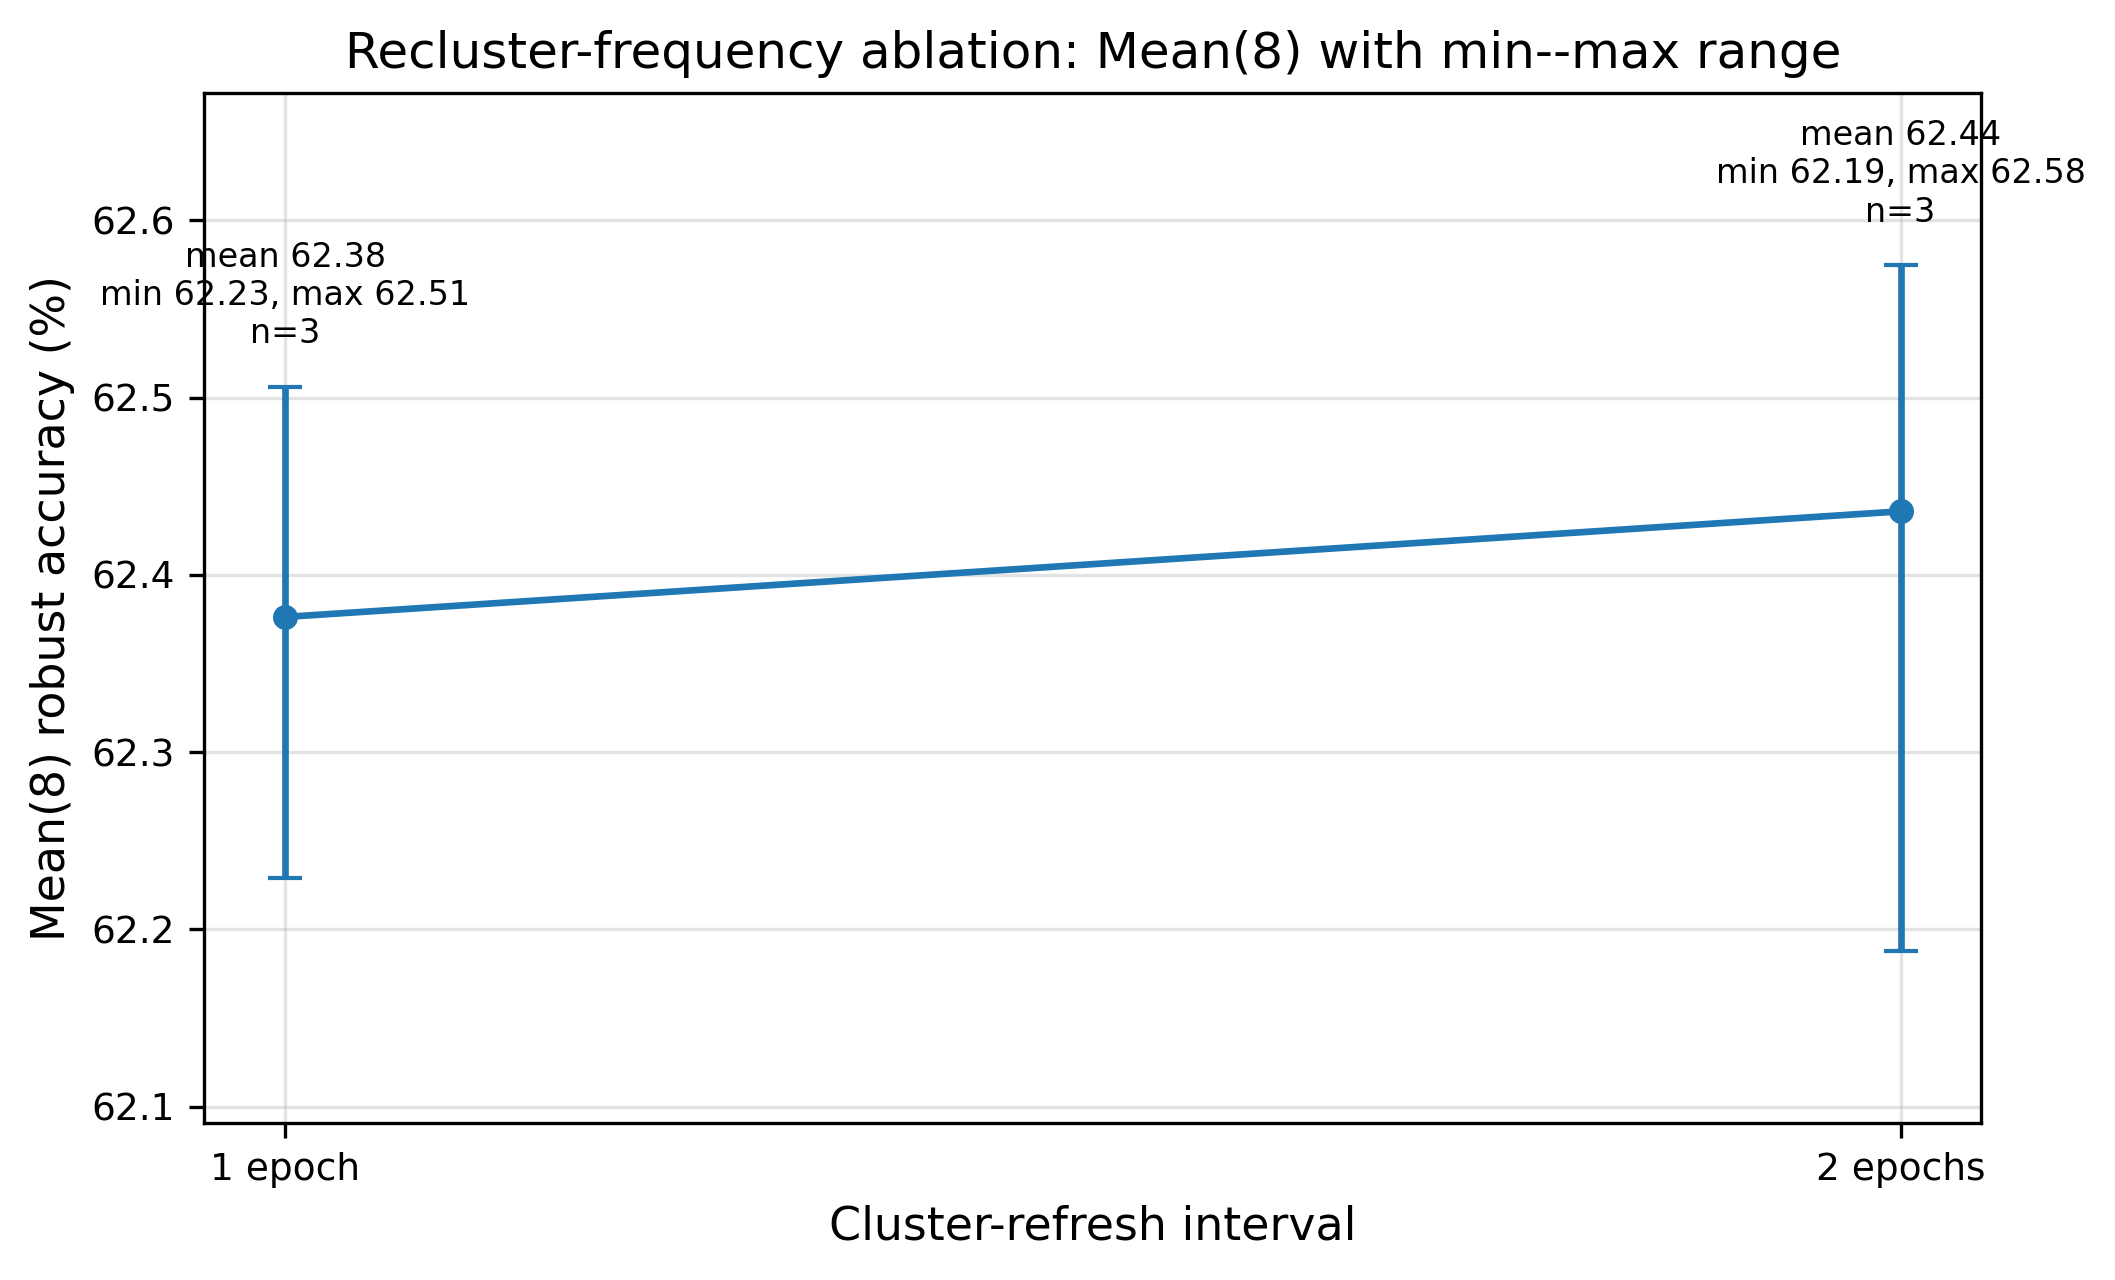
\includegraphics[width=0.82\linewidth]{figures/ablations/ablation_recluster_frequency.png}
    \caption{Sensitivity of AttackDRO++ to the cluster-refresh interval. Points show Mean(8) robust accuracy with the min-to-max range across available runs; Mean(8) is computed over the eight non-AutoAttack evaluation attacks. The two refresh schedules produce similar results, so the default two-epoch schedule is retained as a practical stability choice.}
    \label{fig:ch6_ablation_recluster_frequency}
\end{figure}

We retain $R=2$ epochs as the default because it gives comparable robustness
while reducing the frequency of cluster refitting. This is a practical choice:
the ablation suggests that the method is not highly sensitive to the exact
refresh interval, so the less frequent schedule is preferred for stability and
simplicity.

\paragraph{Supplementary architecture check.}
A single-run WRN-28-10 check is reported in Appendix~\ref{app:extras} as
supplementary evidence. This check is not included in the main paired claims
because it does not use the repeated-random-seed protocol of the main ResNet-18
experiments. In that setting, Multi-AT slightly outperforms AttackDRO++ on both
Mean(8) and AutoAttack-$\ell_\infty$, suggesting that the relative benefit of
the proposed grouping strategy may depend on model capacity and should be
evaluated more systematically in future work.

Together, these ablations suggest that the final AttackDRO++ configuration is
not the result of a fragile hyperparameter choice. Moderate clustering
granularity, moderate anchor strength, and a two-epoch refresh schedule provide a
stable practical configuration. The ablations also define the limits of the
current evidence: they support the selected ResNet-18 configuration, but broader
architecture-level conclusions require additional repeated-seed experiments.

% Diagnostics removed from main report outline; keep file for archive only.
% \section{Diagnostics}


\subsection{Embedding Visualization}

\subsection{Clustering Agreement}

\subsection{Cluster Composition Across Attacks and Classes}

\subsection{q Dynamics Across Training}     
Chapter~\ref{chap:results_analysis} evaluated AttackDRO++ through four connected
evidence panels. The aggregate whitebox results first showed that the proposed
method gives modest average and held-out gains relative to Multi-AT while
leaving Worst(8) and the separate AutoAttack checks broadly unchanged. The
per-attack and class-wise drilldowns then clarified where this behavior comes
from: the method acts less like a single-norm specialist and more like a
balanced multi-attack model, although hard animal-class cells under strong
\(\ell_\infty\) attacks remain persistent failure cases.

The graybox analysis tested whether the same pattern survives transferred
attacks from separately trained surrogate checkpoints. It supported the
whitebox interpretation while also showing that transfer accuracy must be read
carefully because specialist models can appear strong when attacks transfer
poorly across threat geometries. Finally, the ablation section examined whether
the observed behavior depends on key design choices, treating cluster count,
anchor strength, and refresh frequency as sensitivity checks rather than
standalone proof.

Overall, the supported conclusion is conservative: within the CIFAR-10 and
ResNet-18 setting studied here, AttackDRO++ improves cross-attack balance over
the uniform multi-attack baseline without establishing superiority on every
attack or extending robustness claims beyond the evaluated protocol. Chapter~\ref{chap:conclusion}
summarizes these findings, states the limitations, and outlines future
extensions.



% End of Chapter 6
